% =====================================================================
%  LLM & GenAI Engineer --- The Memorize-Cold Sheet
%  Built on the Achilles curriculum (github.com/Lourdhu02/achilles)
%  Compile: pdflatex main.tex (twice, for the contents)
% =====================================================================
\documentclass[8pt,twocolumn,a4paper]{extarticle}

% ---------- page ----------
\usepackage[a4paper,top=13mm,bottom=13mm,left=11mm,right=11mm,columnsep=6mm,headsep=3mm,footskip=6mm]{geometry}
\setlength{\columnseprule}{0.2pt}

% ---------- fonts ----------
\usepackage[T1]{fontenc}
\usepackage[sc]{mathpazo}
\linespread{1.04}
\usepackage[scaled=0.90]{helvet}
\renewcommand{\ttdefault}{lmtt}
\usepackage{microtype}

% ---------- maths, tables ----------
\usepackage{amsmath,amssymb,bm}
\usepackage{booktabs,tabularx,array,multirow}
\usepackage{enumitem}
\setlist{nosep,leftmargin=1.1em,labelsep=0.4em}
\setlist[itemize]{label={\color{acc}\tiny$\blacktriangleright$}}
\renewcommand{\arraystretch}{1.12}
\setlength{\tabcolsep}{3pt}

% ---------- colour ----------
\usepackage[dvipsnames]{xcolor}
\definecolor{acc}{HTML}{1F4E79}   % deep blue
\definecolor{acc2}{HTML}{B5462B}  % rust
\definecolor{acc3}{HTML}{2E7D4F}  % green
\definecolor{ink}{HTML}{222222}
\definecolor{soft}{HTML}{F3F6FA}
\definecolor{soft2}{HTML}{FBF4EE}
\definecolor{rule}{HTML}{9DB3C8}
\definecolor{mute}{HTML}{6B7785}
\color{ink}

% ---------- diagrams ----------
\usepackage{tikz}
\usetikzlibrary{arrows.meta,positioning,calc,fit,shapes.geometric,backgrounds,decorations.pathreplacing,matrix}
\usepackage{pgfplots}
\pgfplotsset{compat=1.16}
\tikzset{
  >={Stealth[length=1.6mm]},
  box/.style={draw=acc,rounded corners=1pt,line width=0.5pt,inner sep=2pt,minimum height=4.2mm,font=\scriptsize,align=center,fill=white},
  sbox/.style={box,fill=soft},
  hbox/.style={box,draw=acc2,fill=soft2},
  gbox/.style={box,draw=acc3,fill=acc3!8},
  lab/.style={font=\scriptsize\color{mute},align=center},
  arr/.style={->,draw=acc,line width=0.5pt},
  darr/.style={->,draw=acc2,line width=0.5pt,dashed},
}

% ---------- boxes ----------
\usepackage[most]{tcolorbox}
\tcbset{
  base/.style={enhanced,breakable,boxrule=0pt,arc=0pt,outer arc=0pt,
    left=3pt,right=3pt,top=2pt,bottom=2pt,before skip=3pt,after skip=4pt,
    fonttitle=\sffamily\bfseries\scriptsize,coltitle=white,
    toptitle=0.5pt,bottomtitle=0.5pt,lefttitle=3pt},
}
% Interview Q&A block
\newtcolorbox{qa}[1][]{base,colback=soft,borderline west={1.6pt}{0pt}{acc},
  before upper={{\sffamily\bfseries\scriptsize\color{acc}INTERVIEW Q\&A\enspace{\color{mute}\textbar}\enspace\MakeUppercase{#1}}\par\smallskip}}
% Must-memorize facts
\newtcolorbox{mem}[1][Memorize]{base,colback=soft2,borderline west={1.6pt}{0pt}{acc2},
  before upper={{\sffamily\bfseries\scriptsize\color{acc2}\MakeUppercase{#1}}\par\smallskip}}
% Traps
\newtcolorbox{trap}[1][Traps]{base,colback=white,borderline west={1.6pt}{0pt}{acc3},
  before upper={{\sffamily\bfseries\scriptsize\color{acc3}\MakeUppercase{#1}}\par\smallskip}}

% One question/answer pair
\newcounter{qn}
\newcommand{\Q}[2]{\refstepcounter{qn}%
  \par\noindent{\sffamily\bfseries\color{acc}Q\theqn.}~{\bfseries #1}\par
  \noindent\hangindent=0.9em\hangafter=0{#2}\par\vspace{2.2pt}}
% Rapid-fire single line
\newcommand{\RF}[2]{\par\noindent\hangindent=0.9em\hangafter=1{\bfseries #1}\;{\color{mute}$\to$}\;#2\par}

% ---------- headings ----------
\usepackage{titlesec}
\titleformat{\section}{\sffamily\bfseries\large\color{acc}}{\thesection}{0.5em}{}[{\color{acc}\titlerule[0.6pt]}]
\titlespacing*{\section}{0pt}{6pt}{3pt}
\titleformat{\subsection}{\sffamily\bfseries\normalsize\color{acc}}{\thesubsection}{0.45em}{}
\titlespacing*{\subsection}{0pt}{4pt}{1.5pt}
\titleformat{\paragraph}[runin]{\sffamily\bfseries\small\color{acc2}}{}{0pt}{}
\titlespacing*{\paragraph}{0pt}{2pt}{0.6em}
\setcounter{secnumdepth}{2}

% ---------- header / footer ----------
\usepackage{fancyhdr}
\pagestyle{fancy}
\fancyhf{}
\renewcommand{\headrulewidth}{0.3pt}
\renewcommand{\headrule}{{\color{rule}\hrule width\headwidth height\headrulewidth}}
\fancyhead[L]{\sffamily\scriptsize\color{mute}LLM \& GenAI Engineer --- memorize-cold sheet}
\fancyhead[R]{\sffamily\scriptsize\color{mute}\nouppercase{\leftmark}}
\fancyfoot[C]{\sffamily\scriptsize\color{mute}\thepage}
\renewcommand{\sectionmark}[1]{\markboth{\thesection\ \ #1}{}}

\usepackage[hidelinks]{hyperref}
\hypersetup{pdftitle={LLM and GenAI Engineer: memorize-cold sheet},pdfauthor={Achilles}}
\usepackage{xurl}
\usepackage{listings}
\usepackage{needspace}
\lstset{language=Python,basicstyle=\ttfamily\fontsize{6.6}{7.6}\selectfont,keywordstyle=\color{acc}\bfseries,commentstyle=\color{mute}\itshape,stringstyle=\color{acc2},backgroundcolor=\color{soft},frame=leftline,framerule=1.2pt,rulecolor=\color{acc},xleftmargin=4pt,framexleftmargin=3pt,aboveskip=2pt,belowskip=3pt,columns=fullflexible,keepspaces=true,showstringspaces=false,breaklines=true}

% ---------- small helpers ----------
\newcommand{\KL}{\mathrm{KL}}
\newcommand{\E}{\mathbb{E}}
\newcommand{\softmax}{\mathrm{softmax}}
\newcommand{\tb}[1]{\textbf{#1}}
\newcommand{\hl}[1]{{\color{acc2}\textbf{#1}}}
\newcommand{\ra}{\,{\color{mute}$\rightarrow$}\,}
\newcommand{\lab}[1]{{\color{mute}\scriptsize[#1]}}
\newcommand{\cn}[1]{{\color{mute}\,[#1]}}
\newcolumntype{L}{>{\raggedright\arraybackslash}X}
\newcommand{\tsmall}{\scriptsize}

\begin{document}
\twocolumn[{%
\begin{tikzpicture}[remember picture,overlay]
\fill[acc] ($(current page.north west)+(0,-0mm)$) rectangle ($(current page.north east)+(0,-4mm)$);
\end{tikzpicture}
\vspace*{1mm}
{\sffamily\bfseries\fontsize{19}{21}\selectfont\color{acc}LLM \& GenAI Engineer}\\[1mm]
{\sffamily\large\color{acc2}The memorize-cold sheet: what you must be able to answer in your sleep}\\[1.5mm]
{\small\color{mute}Built on the Achilles curriculum (modules 00--10, labs 01--18) and extended across the field. Interview-style Q\&A first, derivations only where the answer \emph{is} the derivation. Numbers are for bf16 on an H100 unless stated. Snapshot: October 2026.}
\vspace{2mm}
{\color{rule}\hrule height 0.4pt}
\vspace{3mm}
}]
\thispagestyle{plain}

\section*{How to use this sheet}
\begin{itemize}
\item \textbf{Three passes.} Day 1: read a section. Day 3: cover every answer and say it out loud. Day 7 and 21: only the questions you missed. Spaced repetition beats re-reading.
\item \textbf{Boxes.} {\color{acc}\textbf{Blue}} = interview Q\&A. {\color{acc2}\textbf{Rust}} = numbers and formulas to memorize. {\color{acc3}\textbf{Green}} = traps interviewers use to separate memorizers from people who can do the arithmetic.
\item \textbf{The four numbers of any model card}: $d$ (width), $L$ (layers), $H/H_{kv}$ (query/KV heads), $V$ (vocab). Parameters, FLOPs, KV cache and communication all follow.
\item \textbf{Answer shape} for any ``why'' question: mechanism \ra\ number \ra\ trade-off \ra\ what you would measure.
\item Pair each section with its Achilles lab (\lab{lab NN}) --- understanding shows up in what you build and measure.
\end{itemize}

\begin{mem}[The 12 numbers everyone asks]
\begin{tabularx}{\linewidth}{@{}lL@{}}
$2mkn$ & FLOPs of an $(m{\times}k)(k{\times}n)$ matmul\\
$2N$ / $6N$ & forward / training FLOPs per token ($8N$ with checkpointing)\\
16 B/param & mixed-precision AdamW training state\\
$\approx$295 & H100 bf16 ridge point, FLOP/byte (989 TF/s \,/\, 3.35 TB/s)\\
$\ln V$ & loss at init (10.82 for $V{=}50{,}257$; 11.76 for 128k)\\
$2LH_{kv}d_h b$ & KV bytes per token (Llama-3-8B: 128 KiB)\\
$1/\sqrt{d_h}$ & keeps attention logits unit-variance at init\\
$8d/3$ & SwiGLU hidden size matching a $4d$ GELU MLP\\
$\approx$20 & Chinchilla tokens/param (compute-optimal, training only)\\
$2\frac{n-1}{n}S$ & ring all-reduce bytes per rank\\
$\sqrt{p(1{-}p)/n}$ & SE of an accuracy; $p{=}0.7,n{=}1000\Rightarrow\pm2.8$ pts\\
$0.95^{20}=0.36$ & a 95\%-per-step agent over 20 steps\\
\end{tabularx}
\end{mem}

{\small\tableofcontents}

\section{Math you actually use}
\lab{module 01 \textperiodcentered\ lab 01 autograd}

\begin{mem}[Identities]
\begin{tabularx}{\linewidth}{@{}lL@{}}
\toprule
Matmul VJP & $Y{=}XW$: $\bar X=\bar Y W^\top$, $\bar W = X^\top\bar Y$\\
Softmax Jacobian & $J=\mathrm{diag}(y)-yy^\top$; VJP $\bar z = y\odot(\bar y-\langle\bar y,y\rangle)$\\
Softmax CE & $\bar z=\softmax(z)-\mathrm{onehot}(t)$ \;($\div$$N$ for batch mean)\\
LayerNorm VJP & $\bar x=\frac1\sigma(\bar y-\overline{\bar y}-\hat x\,\overline{\bar y\odot\hat x})$\\
RMSNorm VJP & $\bar x=\frac1r(\bar y-\hat x\,\overline{\bar y\odot\hat x})$\\
gather / sum & VJP is scatter-\textbf{add} / broadcast\\
MLE & $\E_p[-\log q]=H(p)+\KL(p\|q)$\\
Log-derivative & $\nabla\E_{p_\theta}[f]=\E[f\,\nabla\log p_\theta]$\\
Baseline & $\E[b\,\nabla\log p_\theta]=b\nabla\!\sum p_\theta=0$\\
Importance sampling & $\E_p[f]=\E_q[f\,p/q]$\\
Bradley--Terry & $P(a\succ b)=\sigma(r_a-r_b)$\\
KL est.\ ($\rho{=}p/q$, $x{\sim}q$) & $k_1=-\log\rho$; $k_3=\rho-1-\log\rho\ge0$\\
SE of accuracy & $\sqrt{p(1-p)/n}$; 95\% CI $=\pm1.96\,$SE\\
GD on quadratic & stable iff $\eta<2/L$; best $\eta=\frac{2}{L+\mu}$, rate $\frac{\kappa-1}{\kappa+1}$\\
\bottomrule
\end{tabularx}
\end{mem}

\begin{qa}[Calculus and linear algebra]
\Q{Derive $\partial L/\partial z$ for softmax cross-entropy.}{$L=-z_t+\log\sum_k e^{z_k}$, so $\partial L/\partial z_j=-\delta_{jt}+e^{z_j}/\sum_k e^{z_k}$, i.e.\ $\bar z=\softmax(z)-\mathrm{onehot}(t)$. It sums to 0. Frameworks fuse \texttt{log\_softmax} with NLL for exactly this gradient and for numerical stability (log-sum-exp with the max subtracted).}
\Q{Does backprop compute the Jacobian?}{No: it computes vector--Jacobian products. The Jacobian of a $4096^2$ matmul output w.r.t.\ one input has $\sim\!2.8\times10^{14}$ entries. Reverse mode costs a small constant ($\approx2\times$) of the forward regardless of parameter count; forward mode costs one pass per input direction.}
\Q{Derive the matmul VJP.}{Trace trick: $dL=\mathrm{tr}(\bar Y^\top(dX\,W+X\,dW))=\mathrm{tr}((\bar YW^\top)^\top dX)+\mathrm{tr}((X^\top\bar Y)^\top dW)$. Shape check: the gradient has the shape of the variable, and there is only one way to combine the factors into it.}
\Q{Why do the rows of the softmax Jacobian sum to zero?}{Adding a constant to all logits does not change the softmax, so $J\mathbf 1=0$. A saturated (one-hot) softmax has $J\approx0$: no gradient flows. That is why attention scales logits by $1/\sqrt{d_h}$.}
\Q{Two free unit tests for a LayerNorm backward?}{$\sum_j\bar x_j=0$ (shift invariance) and $\sum_j\bar x_j\hat x_j=0$ when $\epsilon=0$ (scale invariance). RMSNorm keeps only the second.}
\Q{Why can FlashAttention's backward skip the $T\times T$ matrix $\bar P$?}{The softmax VJP needs $\langle\bar P_i,P_i\rangle$ per row, which equals $\langle\bar O_i,O_i\rangle$ (swap sums, $\sum_jP_{ij}V_j=O_i$): one length-$d$ dot product per row ($D_i$ in FA-2).}
\Q{What does SVD buy you in LLM work?}{Eckart--Young: the best rank-$r$ approximation keeps the top $r$ singular values (error $\sqrt{\sum_{i>r}\sigma_i^2}$). LoRA bets updates are low rank; Muon replaces $G=U\Sigma V^\top$ by $UV^\top$; spectral norm $\sigma_{\max}$ bounds how much a layer stretches inputs.}
\Q{Two random unit vectors in $d{=}4096$: expected dot product?}{Mean 0, variance $1/d$, std $1/64\approx0.016$: nearly orthogonal. High-dimensional space holds exponentially many almost-orthogonal directions \ra\ the geometric basis of superposition.}
\Q{How do you gradient-check correctly?}{Central differences in float64 with $\epsilon\approx u^{1/3}\approx10^{-5}$, using a random upstream gradient $G$ on $\sum f(x)\odot G$. In float32 you cannot tell a subtle bug from rounding.}
\end{qa}

\begin{qa}[Probability and information]
\Q{Why is pretraining ``just'' minimizing KL?}{Cross-entropy $=H(p_\text{data})+\KL(p_\text{data}\|q_\theta)$ and $H$ is constant, so MLE minimizes forward KL. Loss is in nats/token; divide by $\ln2$ for bits; compare across tokenizers with \emph{bits per byte}.}
\Q{Forward vs reverse KL?}{Forward $\KL(p\|q)$ is \textbf{mode-covering} (punishes $q\approx0$ where $p>0$): SFT, pretraining, classic distillation. Reverse $\KL(q\|p)$ is \textbf{mode-seeking}: RLHF's penalty $\KL(\pi\|\pi_\text{ref})$, on-policy distillation. Example $p=(.5,.5),q=(.9,.1)$: forward 0.511, reverse 0.368 nats. KL is not a distance (asymmetric, no triangle inequality).}
\Q{What is the log-derivative (REINFORCE) trick and why does RL need it?}{$\nabla_\theta\E_{x\sim p_\theta}[f(x)]=\E[f(x)\nabla_\theta\log p_\theta(x)]$. It needs only samples and $\log p$, not a differentiable reward --- so rewards can be unit tests, verifiers or humans.}
\Q{Does a baseline bias the policy gradient?}{No --- it reduces \emph{variance}. $\E[b\nabla\log p_\theta]=0$ for any $b$ independent of the sampled $x$. RLOO uses the mean of the \emph{other} samples; GRPO's group mean includes the sample itself, which only rescales the gradient by $(1-1/G)$.}
\Q{Where does importance sampling show up in LLMs?}{PPO/GRPO ratio $\pi_\theta/\pi_\text{old}$ (reuse rollouts for several steps), speculative decoding's $\min(1,p/q)$, off-policy correction in async RL. Variance explodes when $q$ under-covers $p$ \ra\ clipping.}
\Q{Which KL estimator does GRPO use and why?}{$k_3=\rho-1-\log\rho$: unbiased (since $\E_q[\rho]=1$), always $\ge0$, low variance. Subtlety: differentiating it through sampled tokens gives the gradient of the \emph{other} KL direction --- still a valid regularizer.}
\Q{Entropy, cross-entropy, perplexity?}{$H(p)=-\sum p\log p$; perplexity $=e^{\text{CE}}$ = effective branching factor. PPL 10 $\Leftrightarrow$ loss 2.30 nats. Not comparable across tokenizers.}
\end{qa}

\begin{qa}[Optimization and statistics]
\Q{GD on a quadratic: stable step and convergence?}{Each eigen-direction scales by $(1-\eta\lambda_i)$; stable iff $\eta<2/L$. Best fixed step gives contraction $(\kappa-1)/(\kappa+1)$. $\kappa=100$: GD 0.980/step (350 steps for $10^3\times$), heavy-ball momentum 0.818/step (35 steps) --- the $\sqrt\kappa$ speed-up is why every optimizer has momentum.}
\Q{What is the edge of stability?}{Full-batch GD drives sharpness (top Hessian eigenvalue) up to $\approx2/\eta$ and hovers there while loss keeps falling non-monotonically (Cohen et al.\ 2021).}
\Q{Model A 71.2\%, B 70.0\% on 1{,}000 items. Better?}{Unpaired 95\% CI is $\pm2.8$ pts each --- not established. Use a \textbf{paired} test on per-item differences (shared variance cancels), bootstrap when no formula exists, clustered SEs when items share a document, and report spread over seeds, not the best seed.}
\Q{Critical batch size?}{Below it, doubling batch nearly halves steps; above it, extra batch buys almost nothing (McCandlish et al.\ 2018). It grows as loss falls, so large runs ramp batch size.}
\end{qa}

\section{ML and DL foundations interviewers still ask}
\lab{gap-fill \textperiodcentered\ the screening round before the LLM round}

\begin{center}
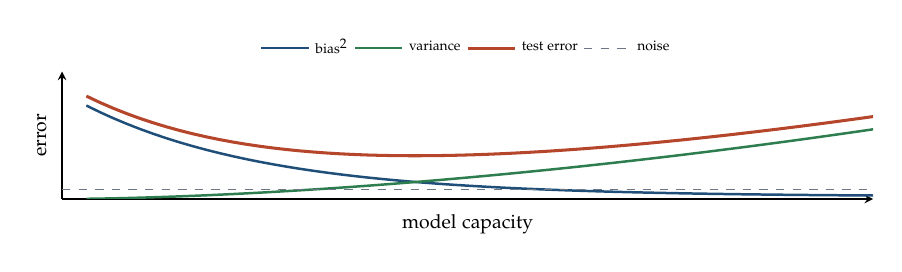
\begin{tikzpicture}
\begin{axis}[width=0.98\columnwidth,height=3.2cm,xmin=0,xmax=10,ymin=0,ymax=1.1,axis lines=left,
  xtick=\empty,ytick=\empty,xlabel={model capacity},ylabel={error},label style={font=\scriptsize},
  legend style={font=\tiny,draw=none,fill=none,at={(0.5,1.02)},anchor=south,legend columns=4}]
\addplot[acc,line width=0.9pt,domain=0.3:10,samples=60]{0.9*exp(-0.45*x)+0.02};\addlegendentry{bias$^2$}
\addplot[acc3,line width=0.9pt,domain=0.3:10,samples=60]{0.012*x^1.7};\addlegendentry{variance}
\addplot[acc2,line width=1.1pt,domain=0.3:10,samples=60]{0.9*exp(-0.45*x)+0.02+0.012*x^1.7+0.08};\addlegendentry{test error}
\addplot[mute,dashed,domain=0:10]{0.08};\addlegendentry{noise}
\end{axis}
\end{tikzpicture}
\end{center}
{\scriptsize\color{mute}Classical U-curve. Over-parameterized nets show \emph{double descent}: error peaks near the interpolation threshold, then falls again with more capacity, data or training.}

\begin{qa}[Learning theory and regularization]
\Q{Bias--variance decomposition?}{$\E[(y-\hat f)^2]=\text{bias}^2+\text{variance}+\sigma^2$. High bias: underfit (bigger model, better features). High variance: overfit (more data, regularize, ensembling, early stopping).}
\Q{L1 vs L2 regularization?}{L2 (ridge, Gaussian prior) shrinks smoothly; L1 (lasso, Laplace prior) drives weights to exactly zero (sparsity) because its subgradient is constant near 0.}
\Q{Why does dropout work?}{Trains an implicit ensemble of thinned subnetworks; prevents co-adaptation; scale by $1/(1-p)$ at train time (inverted dropout) so inference needs no change.}
\Q{BatchNorm vs LayerNorm?}{BN normalizes each feature over the batch (needs running stats, breaks with small/variable batches and autoregressive decoding); LN normalizes each token over features (batch-independent) \ra\ LN/RMSNorm in transformers.}
\Q{Why does Adam generalize differently from SGD?}{Adaptive per-parameter steps converge fast but can find sharper minima in vision; with AdamW and good schedules it is the LLM default. SGD+momentum still common in CNNs.}
\Q{Cross-validation and leakage?}{$k$-fold for small data; split by group/time to avoid leakage (same user, future data); never fit preprocessing on the full set.}
\Q{Class imbalance?}{Use PR-AUC/F1 not accuracy; reweight or resample; focal loss; threshold tuning on a validation set; calibrate afterwards.}
\end{qa}

\begin{mem}[Metrics]
\begin{tabularx}{\linewidth}{@{}lL@{}}
\toprule
precision / recall & $\frac{TP}{TP+FP}$ / $\frac{TP}{TP+FN}$;\ \ F1 $=\frac{2PR}{P+R}$\\
ROC-AUC & P(score pos $>$ score neg); threshold-free; misleading under heavy imbalance\\
PR-AUC & better for rare positives\\
calibration & ECE: $\sum_b\frac{n_b}{n}|\text{acc}_b-\text{conf}_b|$; fix with temperature scaling\\
perplexity & $\exp(\text{mean NLL})$\\
BLEU / ROUGE & $n$-gram precision (brevity penalty) / recall-oriented overlap; weak for LLM outputs\\
BERTScore & token embedding similarity\\
recall@$k$, MRR, nDCG & retrieval: hit in top $k$; $1/\text{rank}$ of first hit; graded, log-discounted\\
WER & speech: (S+D+I)/N\\\bottomrule
\end{tabularx}
\end{mem}

\begin{qa}[Neural network history you'll be asked to connect]
\Q{Why did RNNs/LSTMs lose to transformers?}{Sequential computation (no parallelism over time), vanishing gradients over long ranges (LSTM gates help but don't fix), fixed-size state bottleneck. Attention gives $O(1)$ path length between any two tokens and parallel training.}
\Q{What did attention originally fix (Bahdanau 2014)?}{The seq2seq bottleneck: the decoder attends over all encoder states instead of one context vector.}
\Q{word2vec in one line?}{Skip-gram with negative sampling learns embeddings so that $\sigma(u_o^\top v_c)$ is high for real context pairs and low for sampled negatives; implicitly factorizes a shifted PMI matrix.}
\Q{CNN essentials?}{Local receptive fields, weight sharing, translation equivariance; output size $\lfloor(n+2p-k)/s\rfloor+1$; params $k^2C_\text{in}C_\text{out}$. ResNets made depth trainable with identity skips --- the same idea as the residual stream.}
\Q{What is the universal approximation theorem's catch?}{One hidden layer can approximate any continuous function, but may need exponential width; says nothing about learnability. Depth buys efficiency.}
\Q{Generative vs discriminative?}{Model $p(x,y)$ (or $p(x)$) vs $p(y|x)$. LLMs are generative models used discriminatively via prompting.}
\Q{What is self-supervised learning?}{Labels come from the data: next-token prediction, masked LM (BERT 15\% masking), contrastive (SimCLR, CLIP), masked autoencoding (MAE).}
\Q{Encoder (BERT) pretraining details?}{MLM: mask 15\% (80\% \texttt{[MASK]}, 10\% random, 10\% unchanged); NSP was later shown unnecessary (RoBERTa). Used for embeddings, classification, rerankers.}
\end{qa}

\begin{qa}[Probability refreshers]
\Q{Bayes' rule and why it matters for evals?}{$P(A|B)=P(B|A)P(A)/P(B)$. A 95\%-accurate detector at 1\% base rate has precision $\approx16\%$ --- always ask for the base rate (e.g.\ judge pass rates, safety classifiers).}
\Q{Expected value of a max over $n$ draws?}{Grows with $n$ (best-of-$n$, best seed, best prompt): selection inflates reported scores --- report means, hold out a confirm set.}
\Q{Temperature in softmax?}{$p_i\propto e^{z_i/T}$: $T\to0$ argmax, $T\to\infty$ uniform; entropy increases with $T$.}
\end{qa}

\begin{qa}[Classical ML in one breath]
\RF{Logistic regression loss and gradient?}{BCE; $\nabla_w=X^\top(\sigma(Xw)-y)/n$; convex}
\RF{Linear regression closed form?}{$w=(X^\top X+\lambda I)^{-1}X^\top y$}
\RF{Naive Bayes assumption?}{features conditionally independent given the class}
\RF{SVM objective?}{max margin: hinge loss $+\frac\lambda2\|w\|^2$; kernels via the dual}
\RF{Decision tree split criterion?}{Gini or entropy (information gain); MSE for regression}
\RF{Random forest vs gradient boosting?}{bagging + feature subsampling (variance $\downarrow$) vs sequential fit to residuals/gradients (bias $\downarrow$)}
\RF{Why do GBDTs still win on tabular data?}{handle heterogenous features, missing values, monotone splits; little tuning}
\RF{$k$-means objective and pitfall?}{within-cluster SSE; local optima (k-means++ init), assumes spherical clusters}
\RF{PCA?}{top eigenvectors of the covariance $=$ top right singular vectors of centered $X$}
\RF{$k$-NN complexity?}{no training; $O(nd)$ per query (ANN indexes for scale)}
\RF{EM algorithm?}{alternate posterior over latents (E) and maximize expected log-likelihood (M); monotone in likelihood}
\RF{Curse of dimensionality?}{distances concentrate; volume grows exponentially; need data $\propto e^d$}
\RF{Gaussian MLE?}{$\hat\mu=\bar x$, $\hat\sigma^2=\frac1n\sum(x-\bar x)^2$ (biased; $\frac1{n-1}$ unbiased)}
\RF{A/B test $p$-value?}{P(effect at least this large $\mid$ no true effect); not P(H$_0$ true)}
\end{qa}

\section{Compute and hardware}\label{sec:compute}
\lab{module 02 \textperiodcentered\ lab 03 napkin math}

Every design decision reduces to \textbf{FLOPs, bytes and bandwidth}. Most kernels are limited by moving bytes, not doing math; every optimization below (fusion, tiling, FlashAttention, quantization, KV compression) moves fewer bytes through slow memory.

\begin{center}
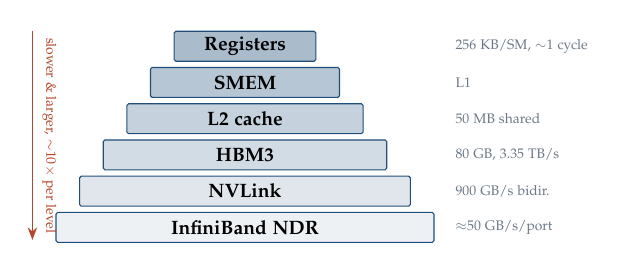
\begin{tikzpicture}[x=1mm,y=1mm,font=\scriptsize]
% memory hierarchy
\foreach \i/\w/\t/\n in {0/18/Registers/{256 KB/SM, $\sim$1 cycle},1/24/SMEM / L1/{$\le$228 KB/SM, you tile here},2/30/L2 cache/{50 MB shared},3/36/HBM3/{80 GB, 3.35 TB/s},4/42/NVLink/{900 GB/s bidir.},5/48/InfiniBand NDR/{$\approx$50 GB/s/port}}{
  \pgfmathsetmacro\y{-\i*4.6}
  \pgfmathtruncatemacro\shade{38-6*\i}
  \draw[draw=acc,fill=acc!\shade!white,rounded corners=0.6pt] (-\w/2,\y) rectangle (\w/2,\y-3.8);
  \node[font=\scriptsize\bfseries] at (0,\y-1.9) {\t};
  \node[anchor=west,font=\tiny\color{mute}] at (25.5,\y-1.9) {\n};
}
\draw[->,acc2,line width=0.6pt] (-27,0) -- (-27,-26.5) node[midway,sloped,above,font=\tiny\color{acc2}]{slower \& larger, $\sim$10$\times$ per level};
\end{tikzpicture}
\end{center}

\begin{center}
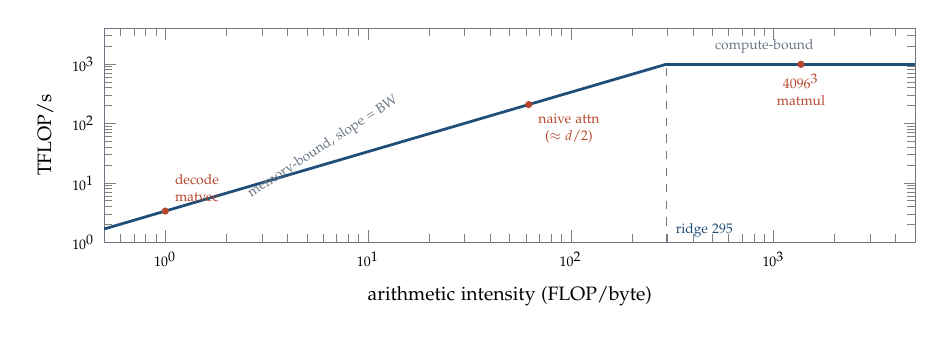
\begin{tikzpicture}
\begin{axis}[width=0.98\columnwidth,height=4.3cm,xmode=log,ymode=log,
  xmin=0.5,xmax=5000,ymin=1,ymax=4000,
  xlabel={arithmetic intensity (FLOP/byte)},ylabel={TFLOP/s},
  label style={font=\scriptsize},tick label style={font=\tiny},
  axis line style={draw=mute},grid=none]
\addplot[acc,line width=1pt,domain=0.5:295,samples=2]{3.35*x};
\addplot[acc,line width=1pt,domain=295:5000,samples=2]{989};
\draw[dashed,mute] (axis cs:295,1) -- (axis cs:295,989);
\node[font=\tiny,acc] at (axis cs:295,1.6) [right] {ridge 295};
\fill[acc2] (axis cs:1,3.35) circle (1.3pt) node[font=\tiny,align=left,above right]{decode\\matvec};
\fill[acc2] (axis cs:62,207.7) circle (1.3pt) node[font=\tiny,align=center,below right]{naive attn\\($\approx d/2$)};
\fill[acc2] (axis cs:1365,989) circle (1.3pt) node[font=\tiny,align=center,below]{$4096^3$\\matmul};
\fill[acc2] (axis cs:2048,989) circle (0pt);
\node[font=\tiny,rotate=33,mute] at (axis cs:6,40) {memory-bound, slope = BW};
\node[font=\tiny,mute] at (axis cs:900,2000) {compute-bound};
\end{axis}
\end{tikzpicture}
\end{center}

\begin{mem}[Roofline]
$t\ge\max\big(\tfrac{\text{FLOPs}}{\text{peak}},\tfrac{\text{bytes}}{\text{BW}}\big)$ + overhead. Intensity $I=$ FLOPs/bytes; ridge $=$ peak/BW.\\
Matmul: $I=\frac{mkn}{mk+kn+mn}$ (bf16). Square: $n/3$ (1365 at 4096). Decode ($m{=}1$): $I\approx1$. Batched decode: $I\approx B$ \ra\ need $B\approx300$ to hit the H100 ridge. Elementwise ops: $I<1$ \ra\ fuse them.\\[2pt]
\begin{tabularx}{\linewidth}{@{}lrrrr@{}}
\toprule
GPU & bf16 dense & HBM & BW & ridge\\\midrule
A100 80G & 312 TF/s & 80 GB & 2.0 TB/s & 150\\
H100 SXM & 989 TF/s & 80 GB & 3.35 TB/s & 295\\
B200 & $\sim$2.2 PF/s & 180 GB & $\sim$8 TB/s & 280\\\bottomrule
\end{tabularx}
\end{mem}

\begin{mem}[Number formats: exponent = range, mantissa = precision]
\begin{tabularx}{\linewidth}{@{}llllL@{}}
\toprule
fmt & s/e/m & max & $\epsilon$ & use\\\midrule
fp32 & 1/8/23 & $3\!\cdot\!10^{38}$ & $1.2\!\cdot\!10^{-7}$ & master weights, optimizer, reductions\\
bf16 & 1/8/7 & $3\!\cdot\!10^{38}$ & $7.8\!\cdot\!10^{-3}$ & default train/infer, no loss scaling\\
fp16 & 1/5/10 & 65{,}504 & $9.8\!\cdot\!10^{-4}$ & needs loss scaling to train\\
e4m3 & 1/4/3 & 448 & 0.125 & FP8 fwd weights/acts\\
e5m2 & 1/5/2 & 57{,}344 & 0.25 & FP8 gradients\\
fp4 e2m1 & 1/2/1 & 6 & 0.5 & MXFP4 (32/blk, pow2 scale), NVFP4 (16/blk, fp8 scale)\\\bottomrule
\end{tabularx}
\end{mem}

\begin{qa}[Compute and memory]
\Q{Why fp32 master weights if you compute in bf16?}{bf16's gap after 1.0 is 0.0078; an Adam update of $10^{-3}$ relative size rounds away (\texttt{bf16(1)+1e-3 == 1}). The fp32 copy accumulates small updates. Same reason accumulations run in fp32 (\texttt{bf16(256)+1 == 256}).}
\Q{Why bf16 over fp16 for training?}{fp16 has 5 exponent bits: overflow above 65{,}504, gradients underflow below $\sim\!6\!\cdot\!10^{-8}$ \ra\ dynamic loss scaling, still fragile on spikes. bf16 has fp32's range.}
\Q{Forward and training FLOPs per token?}{Forward $\approx2N$ (one multiply-add per weight). Backward computes $\bar X$ and $\bar W$, each as big as the forward matmul \ra\ training $\approx6N$; activation checkpointing adds a forward \ra\ $8N$. Attention adds $\approx 6LTd$ per token in training: at 128k context it exceeds $6N$ for an 8B model.}
\Q{Memory to train a 7B model with AdamW?}{16 B/param: bf16 weights 2 + bf16 grads 2 + fp32 master 4 + Adam $m$ 4 + $v$ 4 = 112 GB before activations \ra\ ZeRO/FSDP, 8-bit optimizers or LoRA.}
\Q{Activation memory per layer (GPT-3 style, 16-bit)?}{$sbh(34+5as/h)$ bytes (Korthikanti et al.). The $5as^2b$ term is the attention matrices; FlashAttention removes it. Full checkpointing stores only $2sbh$ per layer at +33\% compute. Don't forget the fp32 logits: $s\cdot b\cdot V\cdot4$ bytes.}
\Q{What is MFU and what is good?}{Model FLOPs (6N + attention) achieved $\div$ peak. Good large runs: 35--55\% (Llama 3 405B: 38--43\%). HFU also counts recomputation. MFU $>100\%$ \ra\ missing \texttt{cuda.synchronize}, tied embedding counted twice, MoE total instead of active params, or wrong peak.}
\Q{Small model runs equally fast on A100 and H100. Why?}{Overhead-bound: kernels too small to fill 132 SMs; CPU launch and Python dominate. Fix with bigger batches, \texttt{torch.compile}, CUDA graphs, fusion --- not a faster GPU.}
\Q{Batch-1 decode speed upper bound for an 8B bf16 model?}{tokens/s $\le$ BW $\div$ weight bytes $=3.35/16\approx$ 200 tok/s, whatever the FLOPs.}
\end{qa}

\begin{mem}[Collectives (ring, $n$ ranks, buffer $S$)]
\begin{tabularx}{\linewidth}{@{}llL@{}}
\toprule
collective & bytes/rank & where\\\midrule
all-reduce & $2\frac{n-1}{n}S$ & DP grads, TP partial sums\\
reduce-scatter & $\frac{n-1}{n}S$ & ZeRO-2/3, FSDP grads\\
all-gather & $\frac{n-1}{n}S$ & ZeRO-3/FSDP params\\
all-to-all & $\frac{n-1}{n}S$ & MoE dispatch, Ulysses SP\\
send/recv & activations & pipeline parallel\\\bottomrule
\end{tabularx}
All-reduce = reduce-scatter + all-gather; per-rank cost $\approx$ independent of $n$. 2 GB grads over 8 GPUs: 55 ms on PCIe 5 (64 GB/s), 7.8 ms on NVLink (450 GB/s/dir).
\end{mem}

\begin{trap}
\begin{itemize}
\item ``Make the math cheaper.'' Cut bytes first; FlashAttention does \emph{more} FLOPs and is faster.
\item Quoting sparse TFLOP/s (H100 ``1{,}979'' assumes 2:4 sparsity). GB vs GiB; Gb vs GB (IB is in gigabits).
\item ``Batching makes decode attention efficient.'' It amortizes weights, not per-sequence KV reads.
\item Timing GPU code without \texttt{torch.cuda.synchronize()} or CUDA events; not discarding warm-up iterations.
\end{itemize}
\end{trap}

\section{GPU and TPU programming}
\lab{lab 06 attention kernels \textperiodcentered\ NVIDIA and Google loops \textperiodcentered\ question bank \S10}

\begin{center}
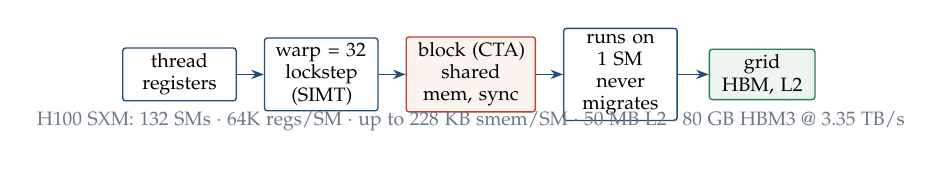
\begin{tikzpicture}[x=1mm,y=1mm,every node/.style={font=\tiny}]
\node[box,text width=13mm] (th) at (0,0) {thread\\registers};
\node[box,text width=13mm] (wp) at (18,0) {warp = 32\\lockstep (SIMT)};
\node[box,text width=15mm,draw=acc2,fill=soft2] (bl) at (37,0) {block (CTA)\\shared mem, sync};
\node[box,text width=13mm] (sm) at (56,0) {runs on 1 SM\\never migrates};
\node[box,text width=12mm,draw=acc3,fill=acc3!8] (gr) at (74,0) {grid\\HBM, L2};
\draw[arr] (th)--(wp); \draw[arr] (wp)--(bl); \draw[arr] (bl)--(sm); \draw[arr] (sm)--(gr);
\node[lab] at (37,-6) {H100 SXM: 132 SMs \textperiodcentered\ 64K regs/SM \textperiodcentered\ up to 228 KB smem/SM \textperiodcentered\ 50 MB L2 \textperiodcentered\ 80 GB HBM3 @ 3.35 TB/s};
\end{tikzpicture}
\end{center}

\begin{qa}[CUDA execution model]
\Q{What is memory coalescing?}{A warp's 32 loads are merged into as few 32-byte sectors as possible. 32 consecutive fp32 values = 128 B = 4 sectors (ideal). Stride-32 access touches 32 sectors for the same useful bytes: $8\times$ less effective bandwidth. Make the fastest-varying thread index walk the contiguous dimension.}
\Q{Shared-memory bank conflicts?}{32 banks, 4 B wide. Threads reading a column of \texttt{float t[32][32]} all hit one bank (32-way conflict, serialized). Pad to \texttt{t[32][33]} so column elements fall in different banks. Broadcast (same address) is free.}
\Q{Compute occupancy for 128 registers/thread.}{$65{,}536/128=512$ threads $=16$ warps per SM, out of a max of 64 warps (25\%). Smem per block and block count limits also apply. More occupancy hides latency but is not the goal: GEMMs trade occupancy for big register tiles (reuse).}
\Q{Warp divergence?}{Threads of one warp taking different branches execute both paths with masks. Make branches uniform per warp (e.g.\ branch on \texttt{warp\_id}, not \texttt{thread\_id\%2}).}
\Q{Arithmetic intensity of a tiled GEMM?}{Per $K$-step a block loads $(B_M+B_N)B_K$ elements and does $2B_MB_NB_K$ FLOPs: $I=\frac{2B_MB_N}{(B_M+B_N)\cdot\text{bytes}}$. $128{\times}128$ bf16: 64 FLOP/B; $32{\times}32$ fp32: 8. Ridge on H100 $\approx$ 295, so bigger tiles + L2 reuse are what make GEMMs compute-bound. One $128{\times}128$, $B_K{=}32$ bf16 stage $=16$ KB smem; 3 pipeline stages $=48$ KB.}
\Q{What do tensor cores need?}{Matrix fragments (e.g.\ $16{\times}8{\times}16$ for bf16 \texttt{mma}), dimensions that are multiples of 8/16 (pad vocab to 128), and for FP8/FP4 per-tensor or per-block scales. Hopper adds \texttt{wgmma} (warpgroup = 4 warps) and TMA async copies; Blackwell adds FP4 and tensor memory.}
\Q{\texttt{\_\_syncthreads()} semantics and pitfalls?}{Barrier for all threads of a \emph{block} (not the grid). Inside a divergent branch it deadlocks or is undefined. Grid-wide sync needs a new kernel launch or cooperative groups.}
\Q{Streams, events, async copies?}{Kernels in different streams may overlap; events time and order them. \texttt{cp.async}/TMA copy global$\to$smem without registers so loads for tile $k{+}1$ overlap compute on tile $k$ (software pipelining, \texttt{num\_stages}).}
\Q{Why does a fused softmax beat three kernels?}{Unfused: max, exp-sum, normalize each read/write the row from HBM. Fused keeps the row in registers/smem: one read, one write. All memory-bound ops in a chain should be fused (bias+act+residual+norm).}
\Q{Nsight Compute says memory 90\%, compute 20\%. Next?}{It's memory-bound: raise reuse (tiling, fusion), cut bytes (lower precision, avoid re-reads), check coalescing and L2 hit rate. Compute 90\%/memory 20\%: you are at the compute roof, so only fewer FLOPs or tensor cores help.}
\Q{What are CUDA graphs for?}{Record a sequence of launches once, replay with one CPU call: removes per-kernel launch overhead ($\sim$5--10\,$\mu$s each), crucial for small-batch decode. Requires static shapes and addresses (hence padded batch buckets).}
\Q{How does NCCL all-reduce scale?}{Ring: each GPU sends $2(n-1)/n\cdot S$ bytes, so time $\approx 2S/\text{BW}$ independent of $n$ (bandwidth-optimal) plus $2(n-1)$ latency hops. Trees for small messages; NVLink/NVSwitch inside a node, IB/RoCE across.}
\end{qa}

\begin{mem}[Triton in eight lines (fused row softmax)]
\begin{lstlisting}
@triton.jit
def softmax_k(X, Y, stride, n, BLOCK: tl.constexpr):
    row = tl.program_id(0)                 # one program per row
    cols = tl.arange(0, BLOCK); mask = cols < n
    x = tl.load(X+row*stride+cols, mask=mask, other=-1e30)
    x = x - tl.max(x, 0); e = tl.exp(x)
    tl.store(Y + row*stride + cols, e / tl.sum(e, 0), mask=mask)
# launch: softmax_k[(rows,)](x, y, x.stride(0), n, BLOCK=1024)
\end{lstlisting}
{\scriptsize You write a program per \emph{tile}; the compiler maps threads, smem, coalescing and tensor-core ops. \texttt{@triton.autotune} benchmarks block sizes, \texttt{num\_warps}, \texttt{num\_stages} per shape key.}
\end{mem}

\begin{mem}[TPU napkin numbers (verify against Cloud TPU docs)]
\begin{tabularx}{\linewidth}{@{}lrrrL@{}}
\toprule
chip & HBM & HBM BW & bf16 FLOP/s & ridge (FLOP/B)\\\midrule
v5e & 16 GB & 0.82 TB/s & 197 T & $\approx$240\\
v5p & 96 GB & 2.8 TB/s & 459 T & $\approx$164\\
v6e (Trillium) & 32 GB & 1.6 TB/s & 920 T & $\approx$575\\\bottomrule
\end{tabularx}\par\smallskip
{\scriptsize $[B,D]\times[D,F]$ matmul intensity $\frac{2BDF}{2BD+2DF+2BF}\approx B$ for $B\ll D,F$: compute-bound only when the per-replica token batch exceeds the ridge (240 tokens on v5e). Sharding scales FLOPs and bandwidth together, so the threshold is per replica. TPUs: systolic MXUs (128$\times$128 or 256$\times$256), ICI torus links, XLA compiles everything.}
\end{mem}

\begin{mem}[PyTorch habit to JAX equivalent]
\begin{tabularx}{\linewidth}{@{}lL@{}}
\toprule
\texttt{loss.backward()} & \texttt{jax.grad(f)(params, batch)} returns a new pytree\\
eager / \texttt{torch.compile} & \texttt{jax.jit}: traces once per shape/dtype; side effects run at trace time only\\
manual batch dim & \texttt{jax.vmap}\\
global RNG & explicit keys, \texttt{jax.random.split(key)}\\
DDP / FSDP & \texttt{Mesh} + \texttt{NamedSharding} + \texttt{jit} (GSPMD); \texttt{shard\_map} for manual collectives\\
Triton & Pallas (TPU and GPU)\\
\texttt{nn.Module}, \texttt{optim} & Flax (NNX), Optax\\
in-place updates & functional: \texttt{x.at[i].set(v)}; \texttt{jax.lax.scan} for loops\\\bottomrule
\end{tabularx}
\end{mem}

\begin{trap}[Classic JAX bugs]
Recompiling on every new sequence length (bucket or pad shapes); Python \texttt{if} on traced values (use \texttt{jnp.where} / \texttt{lax.cond}); reusing a PRNG key; printing inside \texttt{jit} (use \texttt{jax.debug.print}); forgetting \texttt{block\_until\_ready()} when timing (async dispatch).
\end{trap}

\section{Deep learning that matters at scale}\label{sec:train}
\lab{module 03 \textperiodcentered\ labs 01, 02}

\begin{mem}[Defaults you must be able to derive]
\begin{tabularx}{\linewidth}{@{}lL@{}}
\toprule
Kaiming (ReLU) & $\mathrm{Var}(W)=2/n_\text{in}$; LeCun (linear/tanh) $1/n_\text{in}$; Xavier $2/(n_\text{in}{+}n_\text{out})$\\
Residual init & scale out-projections by $1/\sqrt{2L}$ (GPT-2: $0.02/\sqrt{24}=0.0041$)\\
AdamW (LLM) & $\beta{=}(0.9,0.95)$, wd 0.1 (not norms/biases), clip 1.0, $\epsilon{=}10^{-8}$\\
Adam bias corr. & $\hat m_t=m_t/(1-\beta_1^t)$; first step $=\eta\,\mathrm{sign}(g)$\\
Warmup & 1--2\% of steps (or a few thousand)\\
Cosine & decay to $\sim$10\% of peak; needs total steps up front\\
WSD & warmup--stable--decay over last 10--20\%\\
Healthy update/weight & $\sim10^{-3}$ per step\\
Init loss & $\ln V$\\
Optimizer state & SGD 0, SGD+mom 4, AdamW 8, Muon/Lion 4, 8-bit Adam $\sim$2 B/param\\
\bottomrule
\end{tabularx}
\end{mem}

\begin{center}
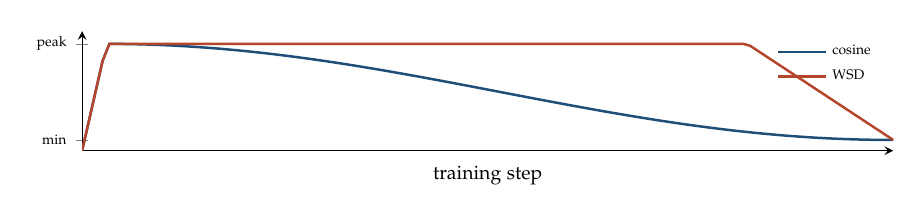
\begin{tikzpicture}
\begin{axis}[width=0.98\columnwidth,height=3.1cm,xmin=0,xmax=100,ymin=0,ymax=1.12,
  axis lines=left,xtick=\empty,ytick={0.1,1},yticklabels={min,peak},
  tick label style={font=\tiny},xlabel={training step},label style={font=\scriptsize},
  legend style={font=\tiny,draw=none,fill=none,at={(0.99,0.98)},anchor=north east},legend cell align=left]
\addplot[acc,line width=0.9pt,domain=0:100,samples=120]{x<3 ? x/3 : 0.1+0.9*0.5*(1+cos(180*(x-3)/97))};
\addlegendentry{cosine}
\addplot[acc2,line width=0.9pt,domain=0:100,samples=120]{x<3 ? x/3 : (x<82 ? 1 : 1-0.9*(x-82)/18)};
\addlegendentry{WSD}
\draw[mute,decorate,decoration={brace,mirror,amplitude=2pt}] (axis cs:0,-0.02) -- (axis cs:3,-0.02);
\end{axis}
\end{tikzpicture}
\end{center}

\begin{qa}[Initialization and normalization]
\Q{Derive Kaiming init.}{$\mathrm{Var}(y_i)=n_\text{in}\mathrm{Var}(W)\E[x^2]$; with $x=\mathrm{ReLU}(z)$ and symmetric $z$, $\E[x^2]=\mathrm{Var}(z)/2$. Stability needs $n_\text{in}\mathrm{Var}(W)/2=1$. 30 ReLU layers of width 256: $N(0,1)$ init explodes to $10^{31}$, $N(0,0.01^2)$ vanishes to $10^{-29}$, Kaiming stays $O(1)$.}
\Q{Why scale residual branches by $1/\sqrt{2L}$?}{The stream is a sum of $2L$ branch outputs (attn + MLP per layer); variance grows as $2Lv$. Scaling each branch std by $1/\sqrt{2L}$ makes total added variance depth-independent.}
\Q{Pre-norm vs post-norm?}{Pre-norm ($x+f(\mathrm{norm}(x))$) keeps an identity gradient path, trains deep stacks without delicate warmup; needs a final norm before the head and the stream norm grows with depth. Post-norm (2017) can be slightly better when it trains but is fragile and needs long warmup.}
\Q{LayerNorm vs RMSNorm?}{RMSNorm drops centering and bias: $x/\sqrt{\mathrm{mean}(x^2)+\epsilon}\cdot g$. Cheaper, equally good; Llama, Qwen, Mistral use it.}
\Q{What is $\mu$P and why do labs use it?}{Width-dependent init and per-layer LR (hidden matrices: Adam LR $\propto1/\text{fan\_in}$; output logits $\times1/\text{width}$; attention $1/d_h$ instead of $1/\sqrt{d_h}$) so hyperparameters tuned on a narrow proxy transfer to the wide model.}
\Q{How can weight decay act as an LR increase?}{Weights feeding a norm are scale-invariant; gradient $\propto1/\|W\|$, so the angular step is $\approx\eta/\|W\|^2$. Decay shrinks $\|W\|$ \ra\ larger effective step; training settles at an equilibrium norm.}
\end{qa}

\begin{qa}[Optimizers and schedules]
\Q{Show the first Adam step has magnitude $\eta$.}{$m_1=(1-\beta_1)g$, $v_1=(1-\beta_2)g^2$; corrected $\hat m_1=g$, $\hat v_1=g^2$ \ra\ update $\eta g/|g|=\eta\,\mathrm{sign}(g)$, independent of gradient scale.}
\Q{Does bias correction make early steps bigger or smaller?}{Depends on betas. Uncorrected with $(0.9,0.999)$: step 1 is $3.16\times$ \emph{too large} (correction shrinks it). With $(0.9,0.95)$: $0.45\times$ (correction enlarges it).}
\Q{Why $\beta_2=0.95$ for LLMs?}{$v$ averages $\approx1/(1-\beta_2)$ steps: 20 vs 1{,}000. After a 10$\times$ gradient spike in steady state: $\beta_2{=}0.999$ gives update 1.81 (amplified); $\beta_2{=}0.95$ gives 0.78 (damped).}
\Q{Adam + L2 vs AdamW?}{L2 adds $\lambda\theta$ to the gradient, then divides by $\sqrt{\hat v}$ --- params with large gradient history get barely regularized. AdamW decouples: $\theta\leftarrow\theta(1-\eta\lambda)-\eta\hat m/(\sqrt{\hat v}+\epsilon)$.}
\Q{What is Muon?}{Momentum on each 2-D hidden matrix, orthogonalized by Newton--Schulz ($USV^\top\to UV^\top$) so every singular direction moves equally; embeddings, head, norms stay on AdamW. 4 B/param state.}
\Q{Why warmup?}{Early curvature is high and Adam's $\hat v$ is a noisy estimate (RAdam's analysis); full steps can throw the model somewhere unrecoverable.}
\Q{When WSD over cosine?}{Unknown final step count, want to continue later, or need several checkpoints at different token budgets from one run (scaling-law sweeps). Branched cooldowns match cosine.}
\Q{How do you scale LR with batch?}{SGD: linearly (up to a point). Adam: $\approx\sqrt k$ for a $k\times$ batch as a start, re-tune near the critical batch.}
\end{qa}

\begin{qa}[Mixed precision and autodiff]
\Q{Describe a bf16 mixed-precision step.}{Matmuls in bf16 on tensor cores; softmax, norms, losses, reductions in fp32; fp32 master weights and optimizer states. No scaler needed.}
\Q{fp16 loss scaling procedure?}{Multiply loss by $S$ ($2^{16}$) before backward; \textbf{unscale before clipping}; on inf/NaN skip the step and halve $S$; double after $\sim$2{,}000 good steps.}
\Q{What does \texttt{loss.backward()} actually do?}{Walks the define-by-run DAG in reverse topological order applying each \texttt{grad\_fn}'s VJP, \emph{summing} where paths merge, \emph{accumulating} into leaf \texttt{.grad} (hence \texttt{zero\_grad}), freeing saved tensors (second backward needs \texttt{retain\_graph}). In-place edits to saved tensors bump a version counter and error.}
\Q{Gradient accumulation normalization?}{Divide by total valid tokens across all micro-batches, not by micro-batch count, or short sequences get over-weighted.}
\Q{Activation checkpointing trade-off?}{Store every $k$-th layer input, recompute the rest: $k\approx\sqrt L$ gives $O(\sqrt L)$ memory for one extra forward ($\approx$+33\% compute). Selective recompute only redoes the cheap-FLOP, big-memory attention parts.}
\end{qa}

\subsection*{Debugging a run from its curves}
\begin{center}
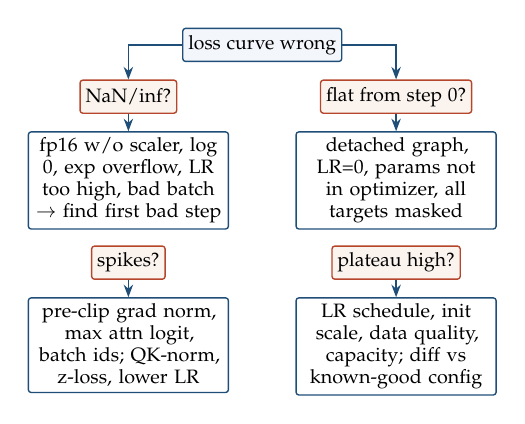
\begin{tikzpicture}[node distance=2.2mm and 3mm,every node/.style={font=\tiny}]
\node[sbox] (a) {loss curve wrong};
\node[hbox,below=of a,xshift=-17mm] (b) {NaN/inf?};
\node[box,below=of b,text width=24mm] (b1) {fp16 w/o scaler, log 0, exp overflow, LR too high, bad batch $\to$ find first bad step};
\node[hbox,below=of a,xshift=17mm] (c) {flat from step 0?};
\node[box,below=of c,text width=24mm] (c1) {detached graph, LR=0, params not in optimizer, all targets masked};
\node[hbox,below=2mm of b1] (d) {spikes?};
\node[box,below=of d,text width=24mm] (d1) {pre-clip grad norm, max attn logit, batch ids; QK-norm, z-loss, lower LR};
\node[hbox,below=2mm of c1] (e) {plateau high?};
\node[box,below=of e,text width=24mm] (e1) {LR schedule, init scale, data quality, capacity; diff vs known-good config};
\draw[arr] (a) -| (b); \draw[arr] (a) -| (c);
\draw[arr] (b)--(b1); \draw[arr] (c)--(c1); \draw[arr] (d)--(d1); \draw[arr] (e)--(e1);
\end{tikzpicture}
\end{center}

\begin{mem}[Symptom $\to$ cause]
\begin{tabularx}{\linewidth}{@{}lL@{}}
\toprule
init loss $\gg\ln V$ & LM head too large, no final norm, $\mu$P multiplier inverted\\
init loss $\ll\ln V$ & label leakage: targets not shifted, causal mask missing\\
stuck at exactly $\ln V$ & output independent of input: detached graph, wrong targets\\
falls then slowly rises & LR too high late, no decay; train/eval mismatch\\
spikes at same step across seeds & bad data shard at a fixed position\\
random growing spikes & attention/output-logit growth \ra\ QK-norm, z-loss\\
drop at each epoch & memorizing repeated data\\
val $<$ train & dropout only in train, leaked/easier eval\\
tokens/s decays & loader starvation, leaks, fragmentation\\
\bottomrule
\end{tabularx}
\end{mem}

\begin{trap}
\begin{itemize}
\item Tuning hyperparameters before you can \textbf{overfit one batch}. Most bugs are data bugs: decode a batch back to text.
\item ``Kaiming is $1/n_\text{in}$.'' That is LeCun; ReLU needs $2/n_\text{in}$.
\item ``Checkpointing halves memory for free.'' +33\% compute, activations only.
\item Clipping before unscaling in fp16: clipping fires every step and the real update is $65{,}536\times$ too small.
\item ``Adam's $\epsilon$ is irrelevant.'' It floors the denominator when gradients are tiny (bf16, big models).
\end{itemize}
\end{trap}

\section{Tokenization}
\lab{module 04 \S1, 05 \S2 \textperiodcentered\ lab 04 tokenizer}

\begin{center}
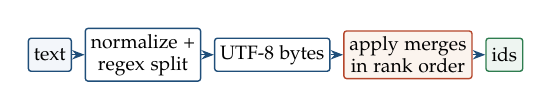
\begin{tikzpicture}[node distance=1.6mm,every node/.style={font=\tiny}]
\node[sbox] (t) {text};
\node[box,right=of t] (p) {normalize +\\regex split};
\node[box,right=of p] (b) {UTF-8 bytes};
\node[hbox,right=of b] (m) {apply merges\\in rank order};
\node[gbox,right=of m] (i) {ids};
\foreach \u/\v in {t/p,p/b,b/m,m/i} \draw[arr] (\u)--(\v);
\end{tikzpicture}

\vspace{1mm}
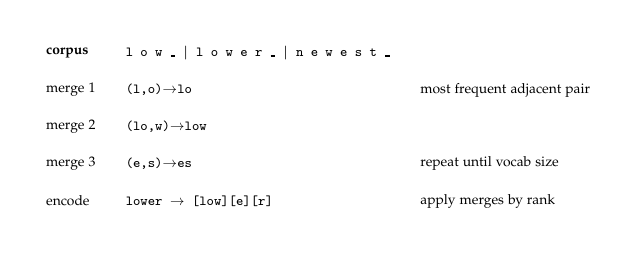
\begin{tikzpicture}[every node/.style={font=\tiny\ttfamily}]
\matrix[matrix of nodes,row sep=0.6mm,column sep=1.5mm,nodes={anchor=west}]{
 \textrm{\bfseries corpus} & l o w \_ \textbar\ l o w e r \_ \textbar\ n e w e s t \_ & \\
 \textrm{merge 1} & (l,o)$\to$lo & \textrm{most frequent adjacent pair}\\
 \textrm{merge 2} & (lo,w)$\to$low & \\
 \textrm{merge 3} & (e,s)$\to$es & \textrm{repeat until vocab size}\\
 \textrm{encode} & lower $\to$ [low][e][r] & \textrm{apply merges by rank}\\
};
\end{tikzpicture}
\end{center}

\begin{mem}[Families]
\begin{tabularx}{\linewidth}{@{}lL@{}}
\toprule
BPE (byte-level) & greedy merges of most frequent pair; 256 base bytes \ra\ no \texttt{<unk>}, ever. GPT-2/4, Llama 3 (tiktoken, 128k)\\
WordPiece & merge pair maximizing $\frac{c(ab)}{c(a)c(b)}$ (likelihood gain); \texttt{\#\#} continuation; BERT\\
Unigram LM & start big, prune tokens whose removal hurts likelihood least; Viterbi/sampled segmentation; SentencePiece (T5, Gemma)\\
SentencePiece & treats input as raw stream incl.\ spaces (\texttt{\_}); BPE or Unigram inside\\
Byte/char-level & no vocab issues, $\sim$4$\times$ longer sequences (ByT5; BLT uses dynamic byte patches)\\
\bottomrule
\end{tabularx}
\end{mem}

\begin{qa}[Tokenizers]
\Q{Why byte-level BPE?}{Every string is representable (256 byte fallback), so no unknown token; merges learned from data compress common sequences. The cost: rare scripts fragment into many bytes.}
\Q{What does the pre-tokenization regex do?}{Splits text (letters, digits in groups of $\le$3, punctuation, whitespace) so merges never cross those boundaries --- e.g.\ ``dog.'' and ``dog!'' share ``dog''. It is frozen into the model.}
\Q{Vocab size trade-off?}{Bigger $V$ \ra\ fewer tokens per text (cheaper long context, faster decode per character) but a bigger embedding + LM head ($2dV$ FLOPs per token; 6.5\% of Llama-3-8B's forward) and rarer, under-trained tokens. 32k (Llama 2) \ra\ 128k (Llama 3) \ra\ 256k (Gemma).}
\Q{What is fertility and why does it matter?}{Tokens per word. High-fertility languages (e.g.\ Telugu under cl100k, split at every vowel sign) pay more per word in cost and context, and get worse quality. Lab 04 measures this.}
\Q{Why are LLMs bad at counting letters or arithmetic?}{They see tokens, not characters; digit grouping is arbitrary (``1234'' may be one or two tokens). Fixes: single-digit tokenization, right-to-left grouping, tool use.}
\Q{What are glitch tokens?}{Tokens in the vocab that almost never appear in training data (e.g.\ ``SolidGoldMagikarp'') \ra\ untrained embeddings \ra\ bizarre behavior. Caused by training the tokenizer on different data than the model.}
\Q{Special tokens and chat templates?}{BOS/EOS, \texttt{<|im\_start|>}-style role markers, tool-call tokens. The template must match training exactly; a missing EOS or a role mismatch silently degrades SFT and inference. Never let user text be parsed into special tokens (injection).}
\Q{Can you change a trained model's tokenizer?}{Not cheaply: embeddings are tied to ids. Adding tokens needs new embedding rows (init as mean of sub-token embeddings) and fine-tuning; swapping tokenizers needs transplant methods + substantial training.}
\Q{How do you compare losses across tokenizers?}{Bits per byte: $\text{BPB}=\frac{\text{total nats}}{\ln2\cdot\#\text{bytes}}$. Per-token loss rewards coarse tokenizers.}
\end{qa}

\begin{trap}
\begin{itemize}
\item Tokenizer and model trained on different normalization (NFC/NFKC) or whitespace handling \ra\ silent quality loss.
\item Trailing-space prompts: ``Answer:\textvisiblespace'' produces a token the model rarely saw before the answer.
\item Counting the input embedding as FLOPs (it is a lookup), but forgetting the LM head (a matmul).
\end{itemize}
\end{trap}

\section{The Transformer, piece by piece}
\lab{module 04 \textperiodcentered\ labs 05 GPT, 06 kernels, 07 KV cache, 18 MoE}

\noindent\begin{minipage}[t]{0.40\columnwidth}\vspace{0pt}\centering
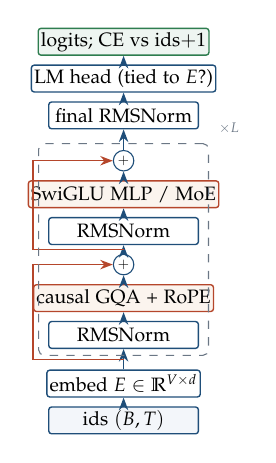
\begin{tikzpicture}[node distance=1.1mm,every node/.style={font=\tiny},
  bx/.style={box,minimum width=19mm,minimum height=3.4mm,inner sep=1pt}]
\node[bx,fill=soft] (ids) {ids $(B,T)$};
\node[bx,above=of ids] (emb) {embed $E\in\mathbb R^{V\times d}$};
\node[bx,above=2.6mm of emb] (n1) {RMSNorm};
\node[bx,draw=acc2,fill=soft2,above=of n1] (att) {causal GQA + RoPE};
\node[circle,draw=acc,inner sep=0pt,minimum size=2.6mm,above=of att] (p1) {$+$};
\node[bx,above=of p1] (n2) {RMSNorm};
\node[bx,draw=acc2,fill=soft2,above=of n2] (mlp) {SwiGLU MLP / MoE};
\node[circle,draw=acc,inner sep=0pt,minimum size=2.6mm,above=of mlp] (p2) {$+$};
\node[bx,above=2.6mm of p2] (nf) {final RMSNorm};
\node[bx,above=of nf] (head) {LM head (tied to $E$?)};
\node[bx,draw=acc3,fill=acc3!8,above=of head] (lo) {logits; CE vs ids$+1$};
\foreach \u/\v in {ids/emb,emb/n1,n1/att,att/p1,p1/n2,n2/mlp,mlp/p2,p2/nf,nf/head,head/lo} \draw[arr] (\u)--(\v);
\coordinate (r0) at ($(emb.north)!0.5!(n1.south)$);
\draw[arr,acc2] (r0) -- ++(-11.5mm,0) |- (p1.west);
\coordinate (r1) at ($(p1.north)!0.5!(n2.south)$);
\draw[arr,acc2] (r1) -- ++(-11.5mm,0) |- (p2.west);
\node[draw=mute,dashed,rounded corners=2pt,fit=(n1)(p2),inner xsep=1.2mm,inner ysep=0.8mm] (blk) {};
\node[font=\tiny\color{mute},anchor=south west] at (blk.north east) {$\times L$};
\end{tikzpicture}
\end{minipage}\hfill
\begin{minipage}[t]{0.58\columnwidth}\vspace{1pt}\small
\textbf{Tokens in, logits out.} Byte-level BPE \ra\ ids \ra\ embedding \ra\ $L$ pre-norm blocks that read from and write to the \textbf{residual stream} $(B,T,d)$ \ra\ final norm \ra\ LM head \ra\ $V$ logits per position.\\[2pt]
One forward pass gives a loss at \emph{every} position at once: decoder-only pretraining is data-efficient per FLOP.\\[2pt]
{\color{acc2}$\blacktriangleright$} Init loss $=\ln V$.\\
{\color{acc2}$\blacktriangleright$} LM head $=2dV$ FLOPs/token (6.5\% of Llama-3-8B).\\
{\color{acc2}$\blacktriangleright$} Tokenizer is frozen forever.\\
{\color{acc2}$\blacktriangleright$} MLP holds $\approx2/3$ of non-embedding params.\\
{\color{acc2}$\blacktriangleright$} Red arrows: identity residual paths (why pre-norm trains deep).
\end{minipage}
\vspace{2mm}

\begin{mem}[Attention]
$\mathrm{Attn}(Q,K,V)=\softmax\!\big(\tfrac{QK^\top}{\sqrt{d_h}}+M\big)V$, $M$ = 0 on/below diagonal, $-\infty$ above. Heads concatenated, projected by $W_O$.\\
$\mathrm{Var}(q\cdot k)=d_h$ for unit-variance entries \ra\ std 11.3 at $d_h{=}128$ \ra\ near one-hot softmax (mean max-prob 0.79 over 1{,}024 keys), Jacobian $\approx0$. Scaling restores unit variance (max-prob 0.017).\\
FLOPs/layer fwd: projections $2T(2d^2+2dH_{kv}d_h)$; scores $2T^2d$; $PV$ $2T^2d$.\\
QK circuit $W_QW_K^\top$ (where to look), OV circuit $W_VW_O$ (what to move); each rank $\le d_h$.
\end{mem}

\begin{center}
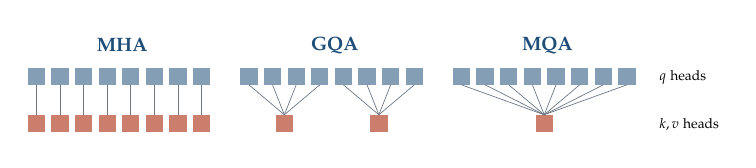
\begin{tikzpicture}[x=1mm,y=1mm,every node/.style={font=\tiny}]
\foreach \name/\x/\g in {MHA/0/1,GQA/27/4,MQA/54/8}{
  \node[font=\scriptsize\bfseries,acc] at (\x+12,9) {\name};
  \foreach \i in {0,...,7}{ \fill[acc!55] (\x+\i*3,4) rectangle ++(2.2,2.2); }
  \pgfmathtruncatemacro\nk{8/\g}
  \pgfmathtruncatemacro\lastk{\nk-1}
  \foreach \j in {0,...,\lastk}{
     \pgfmathsetmacro\cx{\x+(\j*\g+(\g-1)/2)*3}
     \fill[acc2!70] (\cx,-2) rectangle ++(2.2,2.2);
     \foreach \i in {1,...,\g}{ \pgfmathsetmacro\qx{\x+(\j*\g+\i-1)*3+1.1} \draw[mute,line width=0.25pt] (\qx,4) -- (\cx+1.1,0.2);}
  }
}
\node[anchor=west] at (79,5) {$q$ heads};
\node[anchor=west] at (79,-1) {$k,v$ heads};
\end{tikzpicture}
\end{center}

\begin{mem}[KV cache: $2\cdot L\cdot H_{kv}\cdot d_h\cdot$bytes per token]
\begin{tabularx}{\linewidth}{@{}Lrr@{}}
\toprule
variant (Llama-3-8B shape: $L{=}32,d_h{=}128$) & per token & 8k ctx $\times$ 32 seqs\\\midrule
MHA, $H_{kv}{=}32$ & 512 KiB & 128 GiB\\
\textbf{GQA}, $H_{kv}{=}8$ (Llama 3) & \textbf{128 KiB} & 32 GiB\\
MQA, $H_{kv}{=}1$ & 16 KiB & 4 GiB\\
MLA (DeepSeek-V2, 60 layers, 576/layer) & 67.5 KiB & 1.8\% of MHA\\\bottomrule
\end{tabularx}
GQA/MQA/MLA cut KV \textbf{memory and decode bandwidth}, not attention FLOPs.
\end{mem}

\begin{qa}[Attention]
\Q{Why divide by $\sqrt{d_h}$ and not $d_h$?}{Dot product of two $d_h$-dim unit-variance vectors has variance $d_h$; dividing by $\sqrt{d_h}$ gives unit variance \emph{at init}. It does not stop logits growing during training --- QK-norm does. ($\mu$P uses $1/d_h$ for width transfer.)}
\Q{Why multiple heads?}{$H$ heads of size $d/H$ cost the same FLOPs as one head of size $d$ but give $H$ independent attention patterns (low-rank bilinear forms).}
\Q{Why does GQA speed decode but not prefill?}{Decode reads the whole KV cache for one query per head ($I\approx1$, bandwidth-bound); sharing each KV head across $g$ query heads cuts bytes by $g$ ($I\approx g$). Prefill is already compute-bound and FLOPs are unchanged.}
\Q{Why GQA rather than MQA?}{MQA (1 KV head) hurts quality and stability, and must be replicated across TP ranks; GQA-8 keeps near-MHA quality with 4$\times$ less cache and shards cleanly up to TP $=H_{kv}$.}
\Q{Explain MLA.}{Cache a low-rank latent $c_t=W^{DKV}h_t$ ($d_c=512$); $k=W^{UK}c$, $v=W^{UV}c$. Since $q^\top W^{UK}c=(W^{UK\top}q)^\top c$, absorb $W^{UK}$ into the query and $W^{UV}$ into $W_O$ \ra\ attend directly over $c$. RoPE would sit between $W^{UK}$ and $c$ and break absorption \ra\ a small decoupled RoPE key (64-d) shared across heads.}
\Q{Sliding-window attention?}{Local layers cache only $W$ tokens (Mistral; Gemma interleaves local/global). Receptive field grows $L\cdot W$ through depth, but not reliably.}
\Q{Causal mask without explicit positions --- does order leak?}{Some (a token can count predecessors), which is why NoPE works at small scale; but models need explicit positions to be good.}
\end{qa}

\begin{center}
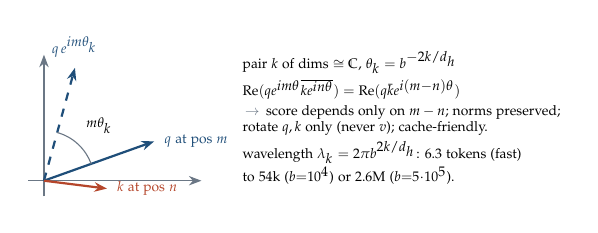
\begin{tikzpicture}[x=1mm,y=1mm,every node/.style={font=\tiny}]
\draw[->,mute] (-2,0)--(20,0); \draw[->,mute] (0,-2)--(0,16);
\draw[acc,line width=0.8pt,->] (0,0) -- (14,5) node[right]{$q$ at pos $m$};
\draw[acc,line width=0.8pt,->,dashed] (0,0) -- ({14*cos(55)-5*sin(55)},{14*sin(55)+5*cos(55)}) node[above]{$q\,e^{im\theta_k}$};
\draw[acc2,line width=0.8pt,->] (0,0) -- (8,-1) node[right]{$k$ at pos $n$};
\draw[mute] (6,2.1) arc (19.6:74.6:6.4);
\node at (7,7) {$m\theta_k$};
\node[anchor=west,align=left,font=\tiny] at (24,8) {pair $k$ of dims $\cong\mathbb C$, $\theta_k=b^{-2k/d_h}$\\[1pt]
$\mathrm{Re}(q e^{im\theta}\overline{ke^{in\theta}})=\mathrm{Re}(q\bar k e^{i(m-n)\theta})$\\[1pt]
\ra\ score depends only on $m-n$; norms preserved;\\ rotate $q,k$ only (never $v$); cache-friendly.\\[1pt]
wavelength $\lambda_k=2\pi b^{2k/d_h}$: 6.3 tokens (fast)\\ to 54k ($b{=}10^4$) or 2.6M ($b{=}5\!\cdot\!10^5$).};
\end{tikzpicture}
\end{center}

\begin{mem}[Context extension: which RoPE pairs to change]
\begin{tabularx}{\linewidth}{@{}lL@{}}
\toprule
PI & positions $m/s$: all $\theta_k/s$; crowds fast pairs \ra\ needs fine-tuning ($\sim$1k steps to 32k)\\
NTK-aware & raise base $b'=b\,s^{d_h/(d_h-2)}$: fast pairs untouched, slowest scaled by $s$\\
YaRN & NTK-by-parts ($\alpha{=}1,\beta{=}32$) + temperature $\sqrt{1/t}=0.1\ln s+1$ ($s{=}16$: logits $\times1.63$)\\
ABF & large base before long training (Code Llama $10^6$; Llama 3 $5\!\cdot\!10^5$)\\
ALiBi / NoPE & linear distance penalty (recency bias) / no positions\\\bottomrule
\end{tabularx}
\end{mem}

\begin{qa}[Positions, MLP, parameters]
\Q{Why does RoPE need PI/NTK/YaRN if it is ``relative''?}{Beyond the training length the slow pairs ($\lambda_k>L$) see rotation angles never seen in training. Fast pairs have seen all angles. Each method is a policy for which pairs to rescale; long-context \emph{data} is still needed to learn to use the range.}
\Q{Two RoPE conventions?}{Interleaved pairs $(2i,2i{+}1)$ (paper, Meta) vs halves $(i,i{+}d_h/2)$ (HF). Loading across them without permuting $W_Q,W_K$ runs fine and outputs garbage.}
\Q{Size SwiGLU's hidden layer.}{$W_\text{down}(\mathrm{SiLU}(W_\text{gate}x)\odot W_\text{up}x)$ has $3df$ params; match $8d^2$ \ra\ $f=8d/3$, rounded (Llama 2: 11{,}008; Llama 3: $\times1.3$ \ra\ 14{,}336). Gated beats ReLU/GELU at equal params; no crisp theory --- say so.}
\Q{Count Llama-3-8B's parameters.}{$d{=}4096,L{=}32,H{=}32,H_{kv}{=}8,f{=}14336,V{=}128256$. Attn $2d^2+2d\cdot1024=41.9$M; MLP $3df=176.2$M; layer 218.1M $\times32=6.98$B; embed+head $2Vd=1.05$B \ra\ \textbf{8.03B}. Classic MHA + 4$d$ GELU: $12d^2$/layer.}
\Q{What do MLPs do, mechanistically?}{Key--value memories: rows of $W_\text{up}/W_\text{gate}$ detect patterns, columns of $W_\text{down}$ write associated outputs; much factual recall lives here.}
\Q{Encoder-only vs decoder-only vs encoder--decoder?}{BERT: bidirectional, MLM, great embeddings/classifiers, no generation. GPT: causal LM, loss at every position, scales best, does everything via prompting. T5/Whisper: encoder reads input bidirectionally, decoder cross-attends; good for translation/speech/seq2seq.}
\end{qa}

\begin{center}
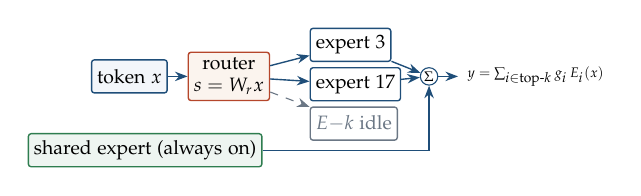
\begin{tikzpicture}[node distance=2mm and 2.5mm,every node/.style={font=\tiny}]
\node[sbox] (x) {token $x$};
\node[hbox,right=of x] (r) {router\\$s=W_rx$};
\node[box,right=5mm of r,yshift=4mm] (e1) {expert 3};
\node[box,right=5mm of r,yshift=-1mm] (e2) {expert 17};
\node[box,right=5mm of r,yshift=-6mm,draw=mute,text=mute] (e3) {$E{-}k$ idle};
\node[gbox,below=5mm of x,xshift=2mm] (sh) {shared expert (always on)};
\node[circle,draw=acc,inner sep=0.5pt,right=19mm of r] (s) {$\Sigma$};
\node[right=of s] (y) {$y=\sum_{i\in\text{top-}k}g_i\,E_i(x)$};
\draw[arr](x)--(r); \draw[arr](r)--(e1); \draw[arr](r)--(e2); \draw[mute,->,dashed](r)--(e3);
\draw[arr](e1)--(s); \draw[arr](e2)--(s); \draw[arr](sh) -| (s);
\draw[arr](s)--(y);
\end{tikzpicture}
\end{center}

\begin{qa}[Mixture of experts]
\Q{Total vs active parameters?}{Mixtral 8$\times$7B: top-2 of 8, 46.7B total / 12.9B active. DeepSeek-V3: 1 shared + 256 routed, top-8, 671B / 37B. FLOPs scale with active, memory with total.}
\Q{Write the Switch load-balancing loss.}{$\mathcal L_\text{aux}=\alpha E\sum_i f_iP_i$; $f_i$ = dispatch fraction (non-differentiable), $P_i$ = mean router prob (differentiable). Balanced value $=\alpha$ ($10^{-2}$). Gradient $\alpha Ef_i$ pushes probability off overloaded experts.}
\Q{Capacity factor?}{Each expert takes $\lceil\mathrm{CF}\cdot kT/E\rceil$ tokens; overflow tokens are dropped (skip the MLP via the residual). $T{=}4096,E{=}64,k{=}2,\mathrm{CF}{=}1.25$ \ra\ 160 slots.}
\Q{Router z-loss and aux-loss-free balancing?}{z-loss $\frac1T\sum(\log\sum e^{s_j})^2$ ($10^{-3}$) keeps router logits small for bf16 stability. DeepSeek-V3: per-expert bias added for top-$k$ \emph{selection only}, nudged by $\pm\gamma$ by load --- a controller instead of a gradient fighting the LM loss.}
\Q{Why fine-grained + shared experts?}{More, smaller experts \ra\ combinatorial flexibility (top-8 of 64: $4.4\times10^9$ combos vs 120 for top-2 of 16) at equal FLOPs; shared experts hold common knowledge so routed ones specialize.}
\Q{Why are MoEs cheap to train but hard to serve?}{All experts resident (671B $\approx$ 671 GB FP8); at small batch each expert sees few tokens \ra\ memory-bound on expert weights; two all-to-alls per layer ($\approx2kd$ elements/token) add latency.}
\end{qa}

\begin{mem}[Stability tricks in configs]
\begin{tabularx}{\linewidth}{@{}lL@{}}
\toprule
QK-norm & RMSNorm on $q,k$ per head: stops attention-logit growth (OLMo 2, Gemma 3)\\
z-loss $10^{-4}\log^2Z$ & output-logit divergence (PaLM)\\
soft-capping $c\tanh(z/c)$ & Gemma 2: attn 50, final 30\\
no biases; no wd on norms & fewer drifting params; gains don't shrink\\\bottomrule
\end{tabularx}
\end{mem}

\begin{qa}[Beyond vanilla attention]
\Q{Why is linear attention an RNN?}{Replace $\exp(q\cdot k)$ by $\phi(q)^\top\phi(k)$: $S_t=S_{t-1}+\phi(k_t)v_t^\top$, $y_t\propto\phi(q_t)^\top S_t$ --- fixed-size state, $O(T)$ time, $O(1)$ memory per token.}
\Q{What makes Mamba ``selective''?}{SSM $h_t=\bar Ah_{t-1}+\bar Bx_t$ with $\Delta,B,C$ functions of $x_t$ and $\bar A=\exp(\Delta A)$: large $\Delta$ resets to focus on now, small $\Delta$ remembers. Parallel scan for training.}
\Q{Why are pure SSMs worse at recall?}{Fixed state: Mamba layer ($d{=}4096$, expand 2, state 16) holds 131k numbers = the KV of just 64 tokens of a GQA layer. Exact copying/needle lookup suffers \ra\ hybrids keep a few attention layers (Jamba, Nemotron-H).}
\end{qa}

\begin{trap}
\begin{itemize}
\item ``$\sqrt{d_h}$ normalizes the output.'' It normalizes pre-softmax logits at init.
\item ``Apply RoPE to $V$.'' Nothing is dotted with $v$.
\item ``SwiGLU hidden $=4d$.'' $\approx8d/3$, rounded.
\item ``MoE is cheaper.'' Per training FLOP at fixed quality; not in memory, comms or small-batch serving.
\item Counting tied embeddings twice; forgetting the LM head's $2dV$ FLOPs.
\end{itemize}
\end{trap}

\section{Pretraining: data, scaling, parallelism}
\lab{module 05 \textperiodcentered\ labs 08 scaling laws, 09 parallelism}

\begin{center}
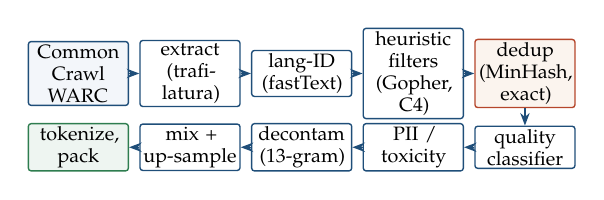
\begin{tikzpicture}[node distance=1.3mm,every node/.style={font=\tiny},
  bx/.style={box,minimum height=4.6mm,text width=12mm,inner sep=1pt}]
\node[bx,fill=soft] (a) {Common Crawl WARC};
\node[bx,right=of a] (b) {extract (trafilatura)};
\node[bx,right=of b] (c) {lang-ID (fastText)};
\node[bx,right=of c] (d) {heuristic filters (Gopher, C4)};
\node[bx,right=of d,draw=acc2,fill=soft2] (e) {dedup (MinHash, exact)};
\node[bx,below=2.2mm of e] (f) {quality classifier};
\node[bx,left=of f] (g) {PII / toxicity};
\node[bx,left=of g] (h) {decontam (13-gram)};
\node[bx,left=of h] (i) {mix + up-sample};
\node[bx,left=of i,draw=acc3,fill=acc3!8] (j) {tokenize, pack};
\foreach \u/\v in {a/b,b/c,c/d,d/e,e/f,f/g,g/h,h/i,i/j} \draw[arr] (\u)--(\v);
\end{tikzpicture}
\end{center}
{\small FineWeb funnel: 96 snapshots \ra\ 36T tokens after base filters \ra\ 20T after per-snapshot MinHash \ra\ \textbf{15T} released; FineWeb-Edu (classifier-kept) $\approx$1.3T and trains much better on knowledge benchmarks. Llama 3 mix $\approx$ 50\% general, 25\% math/reasoning, 17\% code, 8\% multilingual.}

\begin{qa}[Data]
\Q{How does MinHash near-dedup work?}{Shingle docs (word 5-grams); $\Pr[\min h(A)=\min h(B)]=J(A,B)$ (Jaccard). $k=b\cdot r$ hashes in $b$ bands of $r$; candidate if any band fully matches: $P=1-(1-s^r)^b$, threshold $\approx(1/b)^{1/r}$. FineWeb: 112 = 14$\times$8 \ra\ $\sim$0.75 similarity. Cluster candidates, keep one per cluster.}
\Q{Is global dedup always better?}{No (FineWeb): global dedup across 96 crawls removed up to 90\% of old snapshots and barely helped; survivors were disproportionately one-off spam, while good pages recur. Dedup per snapshot.}
\Q{How much can you repeat data?}{Up to $\sim$4 epochs is nearly as good as fresh at fixed compute (Muennighoff 2023); beyond that returns decay to zero. Always tabulate \textbf{epochs per source}: 50B math tokens at 10\% of a 2T run = 4 epochs.}
\Q{How do you decontaminate, and what slips through?}{Drop/flag docs sharing $n$-grams (GPT-3: 13-grams) with test sets; report clean vs contaminated subsets. Paraphrases, translations and forum solutions slip through \ra\ prefer post-cutoff and private evals.}
\Q{What is mid-training / annealing?}{During the final LR decay, upsample highest-quality data (math, code, instruction-like, long docs). Per token it moves benchmarks most.}
\Q{Packing and document masking?}{Concatenate docs with EOS into fixed-length sequences (no padding waste); mask attention across document boundaries (matters most at long context).}
\Q{Role and risk of synthetic data?}{Rephrased web, textbook-style text, reasoning traces are central now; they inherit the generator's blind spots and narrow diversity \ra\ keep a real-data baseline, measure diversity.}
\end{qa}

\begin{mem}[Scaling laws]
{\centering $L(N,D)=E+\dfrac{A}{N^\alpha}+\dfrac{B}{D^\beta}$\qquad(Chinchilla)\par}
$E{=}1.69$, $A{=}406.4$, $B{=}410.7$, $\alpha{=}0.34$, $\beta{=}0.28$.\\
With $C=6ND$: $N^*\propto C^{\beta/(\alpha+\beta)}$, $D^*\propto C^{\alpha/(\alpha+\beta)}$. Approaches 1--2: $a\approx0.5$ \ra\ $\approx$\textbf{20 tokens/param} (Chinchilla = 70B on 1.4T).\\[2pt]
\begin{tabularx}{\linewidth}{@{}lrrrr@{}}
\toprule
$C$ (approach-3 fit) & $N^*$ & $D^*$ & tok/param & loss\\\midrule
$10^{20}$ & 0.64B & 26B & 40 & 2.60\\
$10^{22}$ & 5.2B & 323B & 63 & 2.14\\
$5.76\!\cdot\!10^{23}$ & 32B & 3.0T & 93 & 1.93\\\bottomrule
\end{tabularx}
Inference-aware: minimize $6ND+2NI$. Llama 3 8B saw 15T tokens ($\approx$1{,}900/param) --- correct for a model served billions of times.
\end{mem}

\begin{center}
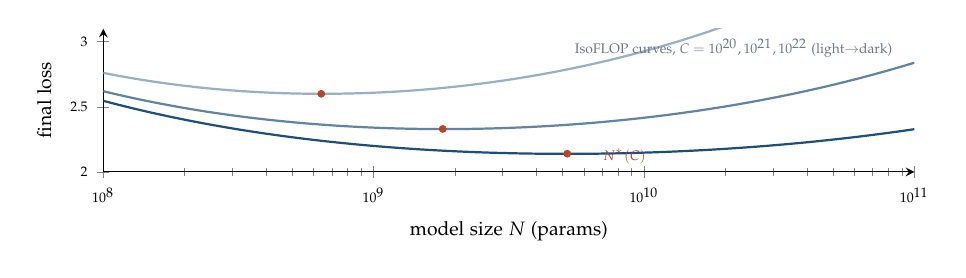
\begin{tikzpicture}
\begin{axis}[width=0.98\columnwidth,height=3.4cm,xmode=log,xmin=1e8,xmax=1e11,ymin=2.0,ymax=3.1,
  xlabel={model size $N$ (params)},ylabel={final loss},label style={font=\scriptsize},tick label style={font=\tiny},axis lines=left]
\foreach \C/\col in {1e20/acc!45,1e21/acc!70,1e22/acc}{
 \edef\tmp{\noexpand\addplot[\col,line width=0.8pt,domain=1e8:1e11,samples=60]{1.69+406.4/x^0.34+410.7/(\C/(6*x))^0.28};}\tmp }
\addplot[only marks,mark=*,mark size=1.2pt,acc2] coordinates {(0.64e9,2.60) (1.8e9,2.33) (5.2e9,2.14)};
\node[font=\tiny,acc2,anchor=west] at (axis cs:6.5e9,2.12) {$N^*(C)$};
\node[font=\tiny,mute,anchor=east] at (axis cs:9e10,2.95) {IsoFLOP curves, $C=10^{20},10^{21},10^{22}$ (light$\to$dark)};
\end{axis}
\end{tikzpicture}
\end{center}

\begin{qa}[Scaling]
\Q{Derive compute-optimal $N^*$.}{Substitute $D=C/6N$, set $dL/dN=0$: $\alpha AN^{-\alpha-1}=\beta B(C/6)^{-\beta}N^{\beta-1}$ \ra\ $N^*=G(C/6)^{\beta/(\alpha+\beta)}$, $G=(\alpha A/\beta B)^{1/(\alpha+\beta)}$.}
\Q{How do you run an IsoFLOP sweep?}{5--9 budgets over $\ge$1.5 decades; 6--10 sizes each trained for $D=C/6N$ \emph{with LR schedule sized to its own length}; fit a parabola of loss vs $\log N$, vertex $=N^*(C)$; fit $\log N^*$ vs $\log C$. Bootstrap CIs on the exponent.}
\Q{Why did Kaplan (2020) and Chinchilla (2022) disagree?}{Kaplan's smaller-scale accounting (excluded embedding params/last-layer FLOPs), warmup and per-scale tuning differences (Porian et al.); not mainly the LR schedule. Kaplan said ``scale $N$ faster''; Chinchilla said scale both equally.}
\Q{Is ``20 tokens/param'' a law?}{No: it is training-compute-optimal under one protocol. Inference-heavy models should train far longer; small cost (6.72B on 2T: loss 2.023 vs 2.016 for optimal 13.2B, at half the serving cost).}
\Q{Do downstream tasks scale smoothly?}{Loss does; tasks are noisier, and discontinuous metrics (exact match) make smooth loss gains look like ``emergence''. Predict loss, then map loss to tasks.}
\end{qa}

\begin{center}
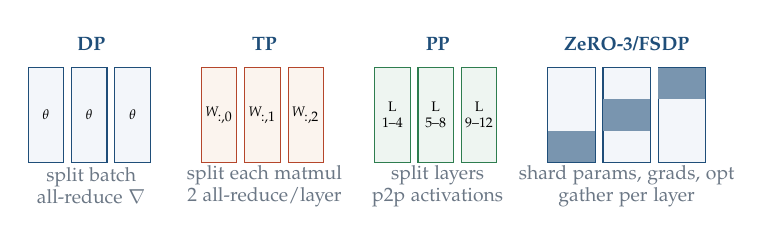
\begin{tikzpicture}[x=1mm,y=1mm,every node/.style={font=\tiny}]
% DP
\node[font=\scriptsize\bfseries,acc] at (8,15) {DP};
\foreach \i in {0,1,2}{\draw[draw=acc,fill=soft] (\i*5.5,0) rectangle ++(4.5,12); \node at (\i*5.5+2.25,6) {$\theta$};}
\node[lab] at (8,-3) {split batch\\all-reduce $\nabla$};
% TP
\node[font=\scriptsize\bfseries,acc] at (30,15) {TP};
\foreach \i in {0,1,2}{\draw[draw=acc2,fill=soft2] (22+\i*5.5,0) rectangle ++(4.5,12); \node at (22+\i*5.5+2.25,6) {$W_{:,\i}$};}
\node[lab] at (30,-3) {split each matmul\\2 all-reduce/layer};
% PP
\node[font=\scriptsize\bfseries,acc] at (52,15) {PP};
\foreach \i in {0,1,2}{\draw[draw=acc3,fill=acc3!8] (44+\i*5.5,0) rectangle ++(4.5,12); \node[align=center] at (44+\i*5.5+2.25,6) {L\\\the\numexpr\i*4+1\relax--\the\numexpr\i*4+4\relax};}
\node[lab] at (52,-3) {split layers\\p2p activations};
% ZeRO
\node[font=\scriptsize\bfseries,acc] at (76,15) {ZeRO-3/FSDP};
\foreach \i in {0,1,2}{\draw[draw=acc,fill=soft] (66+\i*7,0) rectangle ++(6,12);
  \fill[acc!60] (66+\i*7,\i*4) rectangle ++(6,4);}
\node[lab] at (76,-3) {shard params, grads, opt\\gather per layer};
\end{tikzpicture}
\end{center}

\begin{mem}[Parallelism cheat table]
\begin{tabularx}{\linewidth}{@{}l>{\raggedright\arraybackslash}p{21mm}L@{}}
\toprule
strategy & shards & communication\\\midrule
DP & batch & all-reduce grads, overlapped with backward\\
ZeRO-1/2/3 & opt / +grads / +params & reduce-scatter grads; ZeRO-3 adds param all-gathers (1.5$\times$ DP)\\
TP & matmuls (col, then row) & 2 all-reduces per layer per pass; NVLink only\\
SP & norm/dropout acts by seq & paired with TP\\
PP & layers into $p$ stages & p2p; bubble $\frac{p-1}{m+p-1}$ (16\% at $p{=}4,m{=}16$)\\
CP & sequence inside attention & KV blocks passed around a ring\\
EP & MoE experts & all-to-all dispatch + combine\\\bottomrule
\end{tabularx}
ZeRO per GPU, 7.5B on 64 GPUs: 120 \ra\ 31.4 \ra\ 16.6 \ra\ 1.9 GB. Global batch = DP $\times$ micro-batch $\times$ grad-accum.
\end{mem}

\begin{qa}[Distributed training]
\Q{Order of decisions for a parallel layout?}{(1) Does one replica fit (16 B/param + activations)? If not, shard state in-node (FSDP) or TP $\le$ GPUs/node, then PP across nodes. (2) Does one sequence fit? SP, then CP. (3) Scale throughput with DP/HSDP. (4) Check every collective overlaps or costs $<$10\% of step. Llama 3 405B: TP8 $\times$ PP16 $\times$ CP $\times$ DP, 38--43\% MFU on 16k H100s.}
\Q{Why never TP across nodes?}{Its all-reduces sit on the critical path of every layer; NVLink $\sim$450 GB/s/dir vs IB $\sim$50 GB/s (9$\times$). Example: 17 ms in-node vs 150 ms over IB against 52 ms of compute.}
\Q{Explain Megatron TP for an MLP.}{Split $W_1$ by columns (each GPU computes part of the hidden, elementwise GELU stays local), $W_2$ by rows (partial sums) \ra\ one all-reduce forward, one backward per block. Attention splits by heads.}
\Q{Does ZeRO-2 cost more communication than DP?}{No: all-reduce = reduce-scatter + all-gather; ZeRO-2 does RS of grads + AG of updated params --- same bytes. ZeRO-3/FSDP adds a param all-gather in backward: 1.5$\times$, per micro-batch.}
\Q{How do you shrink the pipeline bubble?}{More micro-batches $m$ (bubble $(p-1)/(m+p-1)$), interleaved/virtual stages, 1F1B schedules, zero-bubble schedules (DualPipe in DeepSeek-V3).}
\Q{Plan a 7B run: 2T tokens, 256 H100s.}{6.72B params ($d$4096, $L$32, GQA-8, $V$128k). $\approx$40.4 GFLOP/token \ra\ $C=8.1\!\cdot\!10^{22}$. At 40\% MFU: 9.2 days, 57k GPU-h. Batch 4.2M tokens, 477k steps, AdamW 3e-4, WSD. HSDP: FSDP in-node $\times$ 32 replicas; $\sim$40 GB/GPU. Checkpoint every $\sim$2 h; spend 5--10\% on proxies first.}
\end{qa}

\begin{qa}[Stability, failures, long context]
\Q{A loss spike on day 6. What do you do?}{Check grad norm and max-logit history one or two steps before, which layers; rewind $\sim$100 steps, skip the offending 200--500 batches (PaLM did $\sim$20 times), lower LR if it repeats. Prevent: QK-norm, z-loss, smaller $\epsilon$.}
\Q{How often to checkpoint?}{Young: $\tau\approx\sqrt{2\delta M}$. $\delta$=1 min, MTBF 8.4 days \ra\ $\sim$155 min. Llama 3 405B: 419 unexpected interruptions in 54 days (78\% hardware).}
\Q{How do you get a 128k-context model?}{Pretrain at 4--8k with a large RoPE base; extend in stages (Llama 3: 6 stages, $\sim$800B tokens) with long docs while keeping short data; CP/ring attention for memory; evaluate with RULER-style tasks and report \emph{effective} context, not needle-only.}
\end{qa}

\begin{trap}
\begin{itemize}
\item Using Chinchilla's published $A,B,\alpha,\beta$ and expecting 20 tokens/param (that fit gives 40--100).
\item ``FSDP costs the same as DP.'' Not ZeRO-3: 1.5$\times$, per micro-batch.
\item Changing GPU count and silently changing global batch (= changing the optimization).
\item Treating hardware failure as rare: at 16k GPUs it is daily; restart is part of the design.
\end{itemize}
\end{trap}

\section{Post-training: SFT, PEFT, RLHF, DPO, GRPO}\label{sec:post}
\lab{module 06 \textperiodcentered\ labs 10 LoRA, 11 DPO, 12 GRPO}

\begin{center}
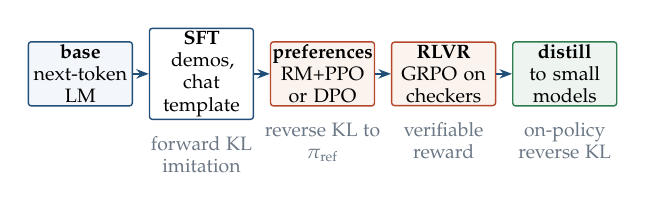
\begin{tikzpicture}[node distance=2mm,every node/.style={font=\tiny},
  bx/.style={box,minimum height=6mm,text width=12.5mm,inner sep=1pt}]
\node[bx,fill=soft] (b) {\textbf{base}\\next-token LM};
\node[bx,right=of b] (s) {\textbf{SFT}\\demos, chat template};
\node[bx,right=of s,draw=acc2,fill=soft2] (p) {\textbf{preferences}\\RM+PPO or DPO};
\node[bx,right=of p,draw=acc2,fill=soft2] (r) {\textbf{RLVR}\\GRPO on checkers};
\node[bx,right=of r,draw=acc3,fill=acc3!8] (d) {\textbf{distill}\\to small models};
\foreach \u/\v in {b/s,s/p,p/r,r/d} \draw[arr] (\u)--(\v);
\node[lab,below=0.8mm of s] {forward KL\\imitation};
\node[lab,below=0.8mm of p] {reverse KL to\\$\pi_\text{ref}$};
\node[lab,below=0.8mm of r] {verifiable\\reward};
\node[lab,below=0.8mm of d] {on-policy\\reverse KL};
\end{tikzpicture}
\end{center}

\begin{qa}[SFT]
\Q{What is the SFT loss, precisely?}{$-\sum_{t\in\text{response}}\log\pi_\theta(y_t|x,y_{<t})$; prompt tokens fed in but masked (label $-100$). It is forward KL to the data \ra\ mode-covering: imitates everything, including mistakes.}
\Q{Most common silent SFT bugs?}{Template mismatch train vs serve; end-of-turn token masked out (pad = eos, collator masks pads) \ra\ model never stops; BOS added twice; loss on prompt tokens. Loss goes down, model gets worse. Decode a batch with masks shown.}
\Q{Packing correctly?}{Block-diagonal causal mask + position ids restarting at 0 per example (varlen FlashAttention takes \texttt{cu\_seqlens}).}
\Q{SFT data recipe?}{Human demos, stronger-model synthetic data, rejection sampling (STaR); decontaminate; mix $>$ size; 1--3 epochs; keep some general chat to limit forgetting. Read 50 random examples first.}
\Q{Why does SFT on stronger-model outputs cause hallucination?}{It teaches the student to state facts the teacher knew but the student does not: it imitates confidence without the knowledge.}
\end{qa}

\begin{center}
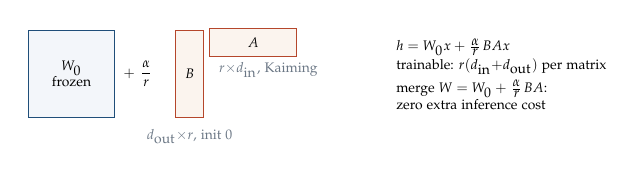
\begin{tikzpicture}[x=1mm,y=1mm,every node/.style={font=\tiny}]
\node[draw=acc,fill=soft,align=center,minimum width=11mm,minimum height=11mm] (w) at (0,0) {$W_0$\\frozen};
\node at (8.5,0) {$+\ \dfrac{\alpha}{r}$};
\node[draw=acc2,fill=soft2,minimum width=3mm,minimum height=11mm] (B) at (15,0) {$B$};
\node[draw=acc2,fill=soft2,minimum width=11mm,minimum height=3mm,anchor=west] (A) at (17.5,4) {$A$};
\node[font=\tiny\color{mute},anchor=north] at (15,-5.8) {$d_\text{out}{\times}r$, init 0};
\node[font=\tiny\color{mute},anchor=west] at (17.5,0.5) {$r{\times}d_\text{in}$, Kaiming};
\node[anchor=west,align=left] at (40,0) {$h=W_0x+\tfrac{\alpha}{r}BAx$\\[1pt]trainable: $r(d_\text{in}{+}d_\text{out})$ per matrix\\[1pt]merge $W=W_0+\tfrac{\alpha}{r}BA$:\\zero extra inference cost};
\end{tikzpicture}
\end{center}

\begin{qa}[Parameter-efficient fine-tuning]
\Q{Why init $B=0$, $A$ random?}{$BA=0$ so training starts exactly at the base model. Both random \ra\ perturbed start; both zero \ra\ no gradient for either ($\nabla A\propto B^\top$, $\nabla B\propto A^\top$).}
\Q{Why the $\alpha/r$ scale?}{Keeps update magnitude roughly independent of $r$ at fixed $\alpha$. rsLoRA uses $\alpha/\sqrt r$ so higher ranks actually learn more.}
\Q{Where to put LoRA, and what LR?}{All linear layers incl.\ MLP (attention-only underperforms). LR $\approx10\times$ full fine-tuning. Qwen2.5-0.5B, $r{=}16$ all 7 linears: 8.8M params (1.8\%).}
\Q{What can't LoRA do?}{On large continued-pretraining-style data (code, math at scale) it learns less --- and forgets less. For RL it matches full FT even at tiny rank (an episode carries few bits).}
\Q{Explain QLoRA.}{Frozen base in \textbf{NF4} (16 levels at normal quantiles, block 64 absmax), dequantized to bf16 per matmul; bf16 LoRA on top; double quantization of scales; paged optimizers. $\approx$4.5 bits/param \ra\ 7--8B on an 8 GB card.}
\Q{Serving 1{,}000 customer fine-tunes?}{Keep one base; batch requests with different adapters in one forward (S-LoRA, Punica). Alternatives: prefix/prompt tuning, IA$^3$, DoRA (magnitude/direction split).}
\end{qa}

\begin{mem}[RLHF objective and its closed form]
{\centering $\displaystyle\max_\pi\ \E_{y\sim\pi}[r(x,y)]-\beta\,\KL(\pi\|\pi_\text{ref})\ \Rightarrow\ \pi^*(y|x)=\tfrac{1}{Z(x)}\pi_\text{ref}(y|x)\,e^{r(x,y)/\beta}$\par}\smallskip
RM loss (Bradley--Terry): $-\log\sigma(r_\phi(x,y_w)-r_\phi(x,y_l))$; only differences identified.\\
Per-token PPO reward: $r_t=-\beta\log\frac{\pi_\theta}{\pi_\text{ref}}(y_t)+\mathbb 1[t{=}T]\,r_\phi(x,y)$.\\
PPO-clip: $\E[\min(\rho A,\ \mathrm{clip}(\rho,1{\pm}\varepsilon)A)]$, $\varepsilon{=}0.2$.\\
GAE: $\delta_t=r_t+\gamma V_{t+1}-V_t$, $\hat A_t=\sum_l(\gamma\lambda)^l\delta_{t+l}$.\\
DPO: $-\log\sigma\big(\beta\log\frac{\pi_\theta(y_w)}{\pi_\text{ref}(y_w)}-\beta\log\frac{\pi_\theta(y_l)}{\pi_\text{ref}(y_l)}\big)$, $\beta\in[0.01,0.5]$.\\
GRPO: $\hat A_i=\frac{r_i-\text{mean}(r)}{\text{std}(r)}$ per group of $G$; PPO-clip; $-\beta\,k_3$.
\end{mem}

\begin{center}
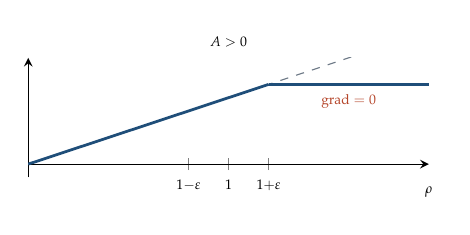
\begin{tikzpicture}
\begin{axis}[width=0.55\columnwidth,height=3.1cm,xmin=0,xmax=2,ymin=-0.2,ymax=1.6,axis lines=middle,
  xtick={0.8,1,1.2},xticklabels={$1{-}\varepsilon$,1,$1{+}\varepsilon$},ytick=\empty,
  tick label style={font=\tiny},title={\tiny $A>0$},title style={yshift=-2mm},
  xlabel={\tiny$\rho$},xlabel style={at={(1,0)},anchor=north}]
\addplot[mute,dashed,domain=0:2]{x};
\addplot[acc,line width=1pt,domain=0:1.2]{x};
\addplot[acc,line width=1pt,domain=1.2:2]{1.2};
\node[font=\tiny,acc2] at (axis cs:1.6,0.95) {grad $=0$};
\end{axis}
\end{tikzpicture}\hfill
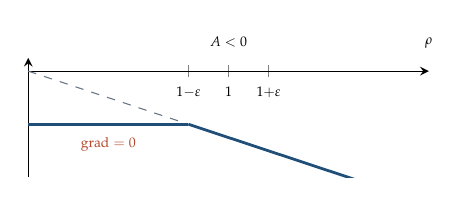
\begin{tikzpicture}
\begin{axis}[width=0.55\columnwidth,height=3.1cm,xmin=0,xmax=2,ymin=-1.6,ymax=0.2,axis lines=middle,
  xtick={0.8,1,1.2},xticklabels={$1{-}\varepsilon$,1,$1{+}\varepsilon$},ytick=\empty,
  tick label style={font=\tiny},title={\tiny $A<0$},title style={yshift=-2mm},
  xlabel={\tiny$\rho$},xlabel style={at={(1,1)},anchor=south}]
\addplot[mute,dashed,domain=0:2]{-x};
\addplot[acc,line width=1pt,domain=0:0.8]{-0.8};
\addplot[acc,line width=1pt,domain=0.8:2]{-x};
\node[font=\tiny,acc2] at (axis cs:0.4,-1.1) {grad $=0$};
\end{axis}
\end{tikzpicture}
\end{center}

\begin{qa}[RLHF and PPO]
\Q{What does the PPO clip actually do?}{Removes the incentive to move further \emph{in the improving direction} once $\rho$ leaves $[1-\varepsilon,1+\varepsilon]$ (flat regions above). It never clips harmful moves: with $A<0$ and large $\rho$, $\rho A$ is smaller and its gradient pulls back. It does not bound the change --- monitor clip fraction and KL.}
\Q{Why the KL penalty?}{Keeps the policy where the RM is still accurate, preserves fluency/diversity. Gao et al.: proxy reward keeps rising with KL while gold reward peaks then falls --- Goodhart with a curve.}
\Q{How many models does PPO-RLHF hold?}{Four: policy (train), value (train), reference (frozen), reward (frozen) --- the cost DPO and GRPO remove.}
\Q{GAE $\lambda$?}{$\lambda=0$: one-step TD (low variance, biased by $V$); $\lambda=1$: Monte Carlo (unbiased, high variance). LLMs often use $\gamma=1$.}
\Q{RM accuracy ceiling?}{Inter-annotator agreement (often 65--75\%), not 100\%. RM = SFT model with a scalar head at the last token.}
\Q{RLHF failure modes?}{Reward hacking, length exploitation, sycophancy, mode collapse (track entropy, distinct-$n$).}
\end{qa}

\begin{qa}[DPO]
\Q{Derive DPO in five steps.}{(1) Optimum $\pi^*=\pi_\text{ref}e^{r/\beta}/Z$ (rewrite objective as $-\beta\KL(\pi\|\pi^*)+\beta\log Z$). (2) Invert: $r=\beta\log\frac{\pi^*}{\pi_\text{ref}}+\beta\log Z(x)$. (3) Plug into Bradley--Terry: $Z(x)$ cancels in $r_w-r_l$. (4) Replace $\pi^*$ by $\pi_\theta$, maximize likelihood of preferences. (5) Gradient weights each pair by $\sigma(\hat r_l-\hat r_w)$: mis-ordered pairs dominate.}
\Q{``DPO has no reward model so it optimizes no reward.'' True?}{False: it optimizes the same KL-regularized objective, reward reparameterized through the policy (implicit reward $\beta\log\pi_\theta/\pi_\text{ref}$). It removes the explicit RM and sampling, not the objective.}
\Q{DPO failure modes?}{Likelihood displacement (both chosen and rejected log-probs fall; mass goes elsewhere); deterministic preferences push $\pi(y_l)\to0$ regardless of $\beta$ (IPO fixes); length exploitation (SimPO normalizes); off-policy pairs (online/iterative DPO is better).}
\Q{DPO debugging checklist?}{Same template/prompt for chosen and rejected; accuracy up while chosen log-prob collapses?; chosen systematically longer?; $\pi_\text{ref}$ = your SFT model, log-probs summed over response tokens with the shift.}
\end{qa}

\begin{mem}[The preference family]
\begin{tabularx}{\linewidth}{@{}lcL@{}}
\toprule
method & ref? & idea\\\midrule
DPO & yes & closed-form RLHF optimum, $-\log\sigma(\beta h)$\\
cDPO & yes & label smoothing for noisy pairs\\
IPO & yes & regress margin to $1/2\tau$: certain prefs don't blow up\\
KTO & yes & unpaired good/bad labels, prospect theory\\
SimPO & no & length-normalized log-prob + margin $\gamma$\\
ORPO & no & SFT + odds-ratio term in one stage\\
Online DPO & yes & fresh pairs from current policy + judge\\\bottomrule
\end{tabularx}
\end{mem}

\begin{center}
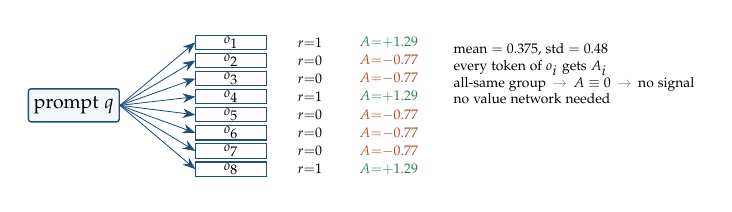
\begin{tikzpicture}[x=1mm,y=1mm,every node/.style={font=\tiny}]
\node[sbox] (q) at (0,0) {prompt $q$};
\foreach \i/\r in {0/1,1/0,2/0,3/1,4/0,5/0,6/0,7/1}{
 \pgfmathsetmacro\yy{8-\i*2.3}
 \node[draw=acc,fill=white,minimum width=9mm,minimum height=1.8mm,inner sep=0pt] (o\i) at (20,\yy) {$o_{\the\numexpr\i+1\relax}$};
 \draw[arr,line width=0.3pt] (q.east) -- (o\i.west);
 \node at (30,\yy) {$r{=}\r$};
 \ifnum\r=1 \node[text=acc3] at (40,\yy) {$A{=}{+}1.29$}; \else \node[text=acc2] at (40,\yy) {$A{=}{-}0.77$}; \fi
}
\node[anchor=west,align=left] at (47,4) {mean $=0.375$, std $=0.48$\\every token of $o_i$ gets $A_i$\\all-same group \ra\ $A\equiv0$ \ra\ no signal\\no value network needed};
\end{tikzpicture}
\end{center}

\begin{qa}[RLVR and GRPO]
\Q{Why GRPO instead of PPO for reasoning?}{A value network for long CoT with one terminal reward is hard to learn and costs a policy-sized model. The group mean is a Monte Carlo estimate of the prompt's value.}
\Q{Why must GRPO rollouts be sampled at temperature $>0$?}{At $T=0$ all $G$ samples are identical \ra\ every advantage 0 \ra\ nothing trains.}
\Q{Known GRPO problems and fixes?}{Length bias from per-sequence $1/|o_i|$ (long wrong answers penalized less per token) \ra\ token-level or constant normalization (DAPO, Dr.\,GRPO). Std normalization over-weights too-easy/too-hard prompts \ra\ drop it (Dr.\,GRPO). Entropy collapse \ra\ clip-higher $\varepsilon_\text{high}{=}0.28$. Zero-variance groups \ra\ dynamic sampling. Truncated answers \ra\ overlong filtering. KL holds back long-CoT \ra\ $\beta{=}0$. Token-ratio noise (MoE) \ra\ sequence-level ratios (GSPO).}
\Q{How do you design an RLVR reward?}{Correctness is the reward, format a gate; normalize and compare answers symbolically; code runs hidden tests in a sandbox; unparseable or multiple answers $=0$; avoid partial credit; keep prompts with pass rate strictly between 0 and 1.}
\Q{Reward hacking examples?}{Listing several answers for a lenient extractor; special-casing visible tests, deleting tests, exiting early with success; flattering an LLM judge; unbounded length. Defence: read samples, stricter held-out grader, track the gap. Don't optimize against the CoT --- it teaches obfuscation.}
\Q{Does RL create reasoning or select it?}{Evidence (Yue et al.): RLVR beats base at pass@1 but base catches up at large $k$ \ra\ mostly sharpening; longer RL (ProRL) may expand it. Know both sides.}
\Q{What to log every RL step?}{Mean reward, zero-variance-group fraction, length split by correct/incorrect, entropy, clip fraction, KL to reference.}
\end{qa}

\begin{qa}[Test-time compute and distillation]
\Q{Ways to buy accuracy with inference compute?}{CoT; self-consistency (majority of $N$); best-of-$N$ with a verifier/RM; PRM-guided beam/tree search; budget forcing (s1: append ``Wait''). Compute-optimal: easy/medium problems gain most; hardest need pretraining compute.}
\Q{ORM vs PRM?}{Outcome RM scores the final answer; process RM scores each step (PRM800K). PRMs select better but are costly to label and hackable as RL rewards.}
\Q{Forward-KL vs reverse-KL vs on-policy distillation?}{Sequence-level KD = SFT on teacher samples (forward, mode-covering). Logit KD at temperature $T$ (scale loss by $T^2$, same tokenizer). On-policy: sample from the student, teacher scores each token \ra\ dense per-token reward, no exposure bias (GKD, Qwen3).}
\Q{Constitutional AI / RLAIF?}{Model critiques and revises its own answers against written principles (SL stage), then RL from AI preference labels; scalable, auditable labeling --- verify against humans.}
\end{qa}

\begin{trap}
\begin{itemize}
\item ``LoRA $r{=}8$ is $8/4096$ of params.'' It is $r(d_\text{in}{+}d_\text{out})$ per matrix, summed over targets.
\item ``SFT loss went down so SFT worked'' / ``reward went up so RL worked.'' Evaluate generations with a stricter grader.
\item ``A baseline biases the gradient.'' Only if it depends on the sampled action.
\item The vocabulary trap: Qwen2.5-0.5B logits for 4$\times$1024 tokens are 2.5 GB in fp32 --- more than its weights. Chunk the loss.
\end{itemize}
\end{trap}

\section{Reasoning models, post-training data, adaptation}
\lab{gap-fill \textperiodcentered\ extends section on post-training}

\begin{center}
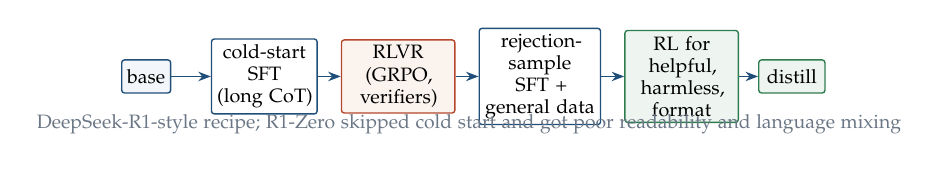
\begin{tikzpicture}[x=1mm,y=1mm,every node/.style={font=\tiny}]
\node[sbox] (b) at (0,0) {base};
\node[box,text width=12mm] (c) at (15,0) {cold-start SFT\\(long CoT)};
\node[box,draw=acc2,fill=soft2,text width=13mm] (r) at (32,0) {RLVR\\(GRPO, verifiers)};
\node[box,text width=14mm] (s) at (50,0) {rejection-sample\\SFT + general data};
\node[box,draw=acc3,fill=acc3!8,text width=13mm] (g) at (68,0) {RL for helpful,\\harmless, format};
\node[gbox,text width=7mm] (d) at (82,0) {distill};
\draw[arr] (b)--(c); \draw[arr] (c)--(r); \draw[arr] (r)--(s); \draw[arr] (s)--(g); \draw[arr] (g)--(d);
\node[lab] at (41,-6) {DeepSeek-R1-style recipe; R1-Zero skipped cold start and got poor readability and language mixing};
\end{tikzpicture}
\end{center}

\begin{qa}[Reasoning and test-time compute]
\Q{What changed with o1 / R1-style models?}{RL on verifiable rewards (math answers, unit tests) teaches long chains of thought with self-checking and backtracking; accuracy scales with both RL compute and the number of thinking tokens at inference.}
\Q{Self-consistency vs best-of-$N$ vs search?}{Self-consistency: majority vote over sampled answers (no verifier, needs a final answer to vote on). Best-of-$N$: pick by a reward model or verifier; gains saturate and the RM gets exploited at large $N$. Search (beam over steps, MCTS) needs a PRM and is costly; sequential revision helps on easy problems, parallel sampling on hard ones.}
\Q{How do you control thinking length?}{Length penalties or budget tokens in RL; ``budget forcing'' at inference (append ``Wait'' to extend, force the answer token to stop, as in s1); train on a mix of short and long traces; route easy queries to no-think mode.}
\Q{What is overthinking and how do you measure it?}{Many tokens spent after the answer is already found, or on trivial problems. Measure accuracy vs tokens curves per difficulty bucket; tokens-to-first-correct; reward shaping on length within correct samples.}
\Q{Is the visible chain of thought faithful?}{Not necessarily: models can use hints without mentioning them. Treat CoT as useful evidence for monitoring, not ground truth; optimizing CoT for appearance can hide misbehavior (obfuscation).}
\Q{Why distill reasoning into small models instead of RL on them?}{SFT on a strong model's traces transfers reasoning cheaply and beat RL directly on small models in R1's report; RL on small models still adds on top once they have the behaviors.}
\Q{What makes a good verifier?}{Exact-match with normalization (math: sympy equivalence), sandboxed unit tests with hidden tests, format checks; guard against reward hacking (special-casing tests, printing expected output, editing the checker).}
\end{qa}

\begin{qa}[Post-training data]
\Q{How do you build an SFT set?}{Define the target behaviors and a taxonomy (tasks, domains, difficulty, safety); seed with expert-written examples; expand with synthetic generation (Self-Instruct, Evol-Instruct, persona-driven) filtered by a judge and verifiers; dedup; decontaminate against evals; balance the mix; a few thousand excellent examples beat many mediocre ones (LIMA).}
\Q{How do you collect preference data?}{Sample 2+ responses per prompt from the current policy (on-policy matters), have raters or a judge pick with a rubric, record margins and ties, measure inter-annotator agreement, refresh iteratively (online/iterative DPO).}
\Q{Annotation guidelines that work?}{Concrete rubric with examples of each grade, tie-break rules, what to do with unsafe/unsure, calibration rounds, gold questions to monitor raters, disagreement adjudication.}
\Q{Synthetic data risks?}{Model collapse from recursive training on own outputs (keep real data in the mix), homogenized style, inherited errors and hallucinations, license/terms of the generator, contamination of evals.}
\Q{How do you filter data quality at scale?}{Heuristics (length, language ID, repetition), perplexity filters, a classifier trained on judge labels (FineWeb-Edu style), dedup (exact + MinHash), PII scrubbing; ablate the filter on small proxy models.}
\end{qa}

\begin{qa}[Adapting a model to your domain]
\Q{Continued pretraining vs SFT?}{CPT on raw domain text (billions of tokens) teaches vocabulary and knowledge; SFT teaches the task format. Typical: CPT with a replay of general data (5--30\%), lower LR with re-warmup, then SFT and preference tuning.}
\Q{How do you prevent catastrophic forgetting?}{Replay general data, lower LR, fewer steps, LoRA (forgets less, learns less), regularize toward the base (KL), evaluate general benchmarks alongside domain ones.}
\Q{What is model merging and when does it work?}{Average weights of fine-tunes from the same base (model soups), task arithmetic (add $\tau=\theta_\text{ft}-\theta_\text{base}$), TIES/DARE resolve sign conflicts and sparsify deltas. Works because fine-tunes stay in one loss basin; fails across different bases.}
\Q{Your fine-tuned model got worse at following instructions. Why?}{Wrong chat template or missing EOS, loss on prompt tokens, overfitting (too many epochs), low-diversity data, LR too high; check with a held-out instruction-following eval and compare to the base.}
\Q{Fine-tuning a model to call your tools?}{Collect real or synthetic multi-turn traces with tool calls, results and final answers in the provider's tool format; include no-tool and error-recovery cases; mask loss on tool outputs; evaluate on exact argument match and end-task success.}
\end{qa}

\begin{mem}[Starting hyperparameters (then sweep)]
\begin{tabularx}{\linewidth}{@{}lL@{}}
\toprule
full SFT (7--8B) & LR 1e-5--2e-5, cosine, warmup 3\%, 2--3 epochs, batch 64--128 seqs, loss on responses only\\
LoRA SFT & LR 1e-4--2e-4, $r$ 16--64, $\alpha=2r$ (or rsLoRA), all linear layers, dropout 0--0.05\\
DPO & LR 5e-7--1e-6 (full) / 5e-6 (LoRA), $\beta=0.1$, 1--2 epochs, watch chosen log-prob\\
GRPO & LR 1e-6, $G=8$--16, temp 1.0, KL 0--0.04, clip 0.2/0.28, max length budgeted\\
CPT & 0.1--0.3$\times$ pretrain peak LR, re-warmup, 5--30\% replay\\\bottomrule
\end{tabularx}
\end{mem}

\section{Inference and serving}\label{sec:inf}
\lab{module 07 \textperiodcentered\ labs 06 kernels, 07 KV cache + sampling, 13 quantization, 14 speculative decoding}

\begin{center}
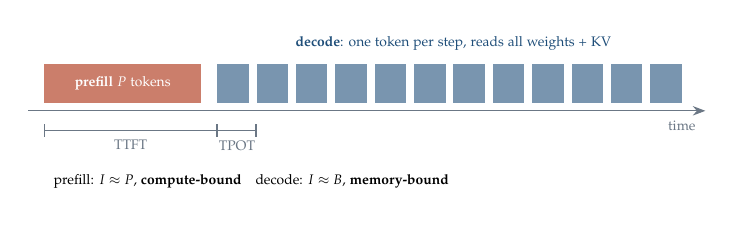
\begin{tikzpicture}[x=1mm,y=1mm,every node/.style={font=\tiny}]
\draw[->,mute] (0,0) -- (86,0) node[below left]{time};
\fill[acc2!70] (2,1) rectangle (22,6); \node[white] at (12,3.5) {\textbf{prefill} $P$ tokens};
\foreach \i in {0,...,11}{ \fill[acc!60] (24+\i*5,1) rectangle ++(4,5); }
\node[acc] at (54,8.5) {\textbf{decode}: one token per step, reads all weights + KV};
\draw[mute,|-|] (2,-2.5) -- (24,-2.5) node[midway,below]{TTFT};
\draw[mute,|-|] (24,-2.5) -- (29,-2.5) node[midway,below]{TPOT};
\node[align=left,anchor=west] at (2,-9) {prefill: $I\approx P$, \textbf{compute-bound}\quad decode: $I\approx B$, \textbf{memory-bound}};
\end{tikzpicture}
\end{center}

\begin{mem}[Serving metrics and the step-time model]
TTFT = queue + prefill. TPOT/ITL = decode step. E2E $=$ TTFT $+(n_\text{out}-1)\cdot$TPOT. Goodput = throughput meeting SLOs.\\[2pt]
{\centering $t_\text{step}\approx\max\Big(\dfrac{2NB}{F_\text{peak}},\ \dfrac{2N+B\,n_\text{ctx}\,s_\text{kv}}{\text{BW}}\Big)+t_\text{overhead}$\par}
Llama-3-8B, H100: batch-1 decode 4.8 ms ($\le$210 tok/s). Batch 64 @ 2k ctx: KV 17.2 GB $>$ weights 16 GB; step $\approx$9.9 ms, $\approx$6{,}500 tok/s. Prefill 1k tokens: 16 TFLOP $\approx$ 16 ms at peak.\\[2pt]
\begin{tabularx}{\linewidth}{@{}lrrL@{}}
\toprule
model (bf16) & KV/token & 32k ctx & shape\\\midrule
Qwen2.5-0.5B & 12 KiB & 0.4 GiB & 24L, 2 kv $\times$ 64\\
Llama-3-8B & 128 KiB & 4 GiB & 32L, 8 kv $\times$ 128\\
Llama-3-70B & 320 KiB & 10 GiB & 80L, 8 kv $\times$ 128\\\bottomrule
\end{tabularx}
For any serving question write three numbers first: weight bytes, KV bytes/token, HBM per GPU.
\end{mem}

\begin{center}
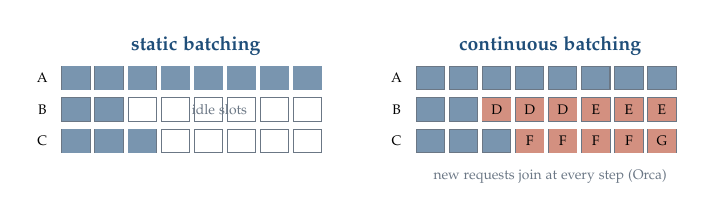
\begin{tikzpicture}[x=1mm,y=1mm,every node/.style={font=\tiny}]
\node[font=\scriptsize\bfseries,acc] at (17,13.5) {static batching};
\node[font=\scriptsize\bfseries,acc] at (62,13.5) {continuous batching};
\foreach \row/\nm in {0/A,1/B,2/C}{
  \node at (-2.5,9.5-\row*4) {\nm};
  \node at (42.5,9.5-\row*4) {\nm};
  \foreach \c in {0,...,7}{\draw[draw=mute,fill=white] (\c*4.2,8-\row*4) rectangle ++(3.6,3);}
}
\foreach \c in {0,...,7}{ \fill[acc!60] (\c*4.2,8) rectangle ++(3.6,3);}
\foreach \c in {0,1}{ \fill[acc!60] (\c*4.2,4) rectangle ++(3.6,3);}
\foreach \c in {0,1,2}{ \fill[acc!60] (\c*4.2,0) rectangle ++(3.6,3);}
\node[mute] at (20,5.5) {idle slots};
\foreach \row in {0,1,2}{ \foreach \c in {0,...,7}{ \draw[draw=mute,fill=acc!60] (45+\c*4.2,8-\row*4) rectangle ++(3.6,3);}}
\foreach \c/\l in {2/D,3/D,4/D,5/E,6/E,7/E}{\fill[acc2!60] (45+\c*4.2,4) rectangle ++(3.6,3); \node at (45+\c*4.2+1.8,5.5){\l};}
\foreach \c/\l in {3/F,4/F,5/F,6/F,7/G}{\fill[acc2!60] (45+\c*4.2,0) rectangle ++(3.6,3); \node at (45+\c*4.2+1.8,1.5){\l};}
\node[mute] at (62,-3) {new requests join at every step (Orca)};
\end{tikzpicture}
\end{center}

\begin{qa}[Serving systems]
\Q{Why is decode slow?}{Not because it is sequential: each step reads every weight and the whole KV cache to make one token per sequence ($I\approx1$). The fix is batching across \emph{users}.}
\Q{Continuous batching?}{Re-form the batch every decode step: finished sequences leave, waiting ones join (Orca). Needs ragged/paged kernels and a per-step scheduler deciding what fits in memory.}
\Q{PagedAttention?}{KV in fixed blocks (16 tokens in vLLM) + per-sequence block table, like virtual memory. Waste $\le$ one partial block per sequence (vs 60--80\% before, $<$4\% after) \ra\ bigger batches. Copy-on-write sharing for parallel samples; preempt by recompute or swap.}
\Q{Prefix caching --- and the timestamp trap?}{Hash full KV blocks by their tokens + everything before (vLLM APC) or keep a radix tree (SGLang RadixAttention). Put stable parts first (system prompt, tools, docs); one timestamp at the top makes every request a miss. Route same-prefix requests to the same replica.}
\Q{Chunked prefill vs disaggregation?}{Chunked (Sarathi): fixed per-step token budget, decode tokens first then a prefill chunk --- no stalls, prefill piggybacks on idle FLOPs. Disaggregated (DistServe, Mooncake): separate prefill and decode pools, ship KV over RDMA (70B: 320 KiB/token \ra\ 330 GB/s at $10^6$ tok/s). Disaggregate at scale with strict TTFT and TPOT SLOs.}
\Q{TP for serving?}{Cuts per-token latency (each GPU streams 1/TP of weights) at the cost of 2 all-reduces per layer; use the smallest TP that fits weights + KV for your batch. Replicas (DP) for throughput.}
\Q{What do CUDA graphs fix?}{CPU launch overhead: hundreds of tiny kernels per small-batch decode step. Record once, replay; one graph per batch-size bucket (pad up). Big win at batch 1--8.}
\Q{``Temperature 0 is deterministic''?}{Not across runs: batch composition changes reduction orders. Needs batch-invariant kernels.}
\Q{How does grammar-constrained decoding work?}{Compile JSON schema/regex to an automaton over the vocab; mask disallowed logits each step; overlap mask computation with the forward. Guarantees it \emph{parses}, not that it is correct.}
\end{qa}

\begin{mem}[Sampling]
logits $/T$ \ra\ top-$k$ (keep $k$ best) \ra\ top-$p$ (smallest set with mass $\ge p$) \ra\ min-$p$ (keep $p_i\ge p_\text{min}\cdot p_\text{max}$) \ra\ sample. $T\to0$: greedy. Repetition/frequency/presence penalties edit logits of seen tokens. Beam search: high-likelihood, bland text; fine for translation/ASR, bad for open-ended chat.
\end{mem}

\begin{center}
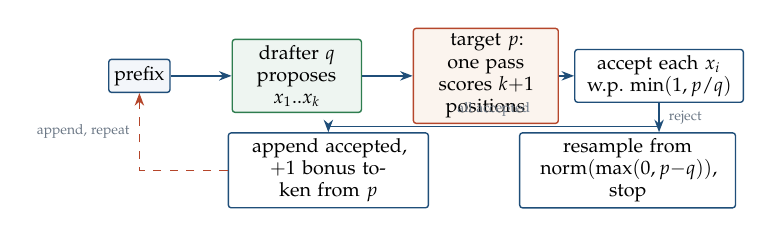
\begin{tikzpicture}[x=1mm,y=1mm,every node/.style={font=\tiny}]
\node[sbox] (pre) at (0,0) {prefix};
\node[box,draw=acc3,fill=acc3!8,text width=15mm] (dr) at (20,0) {drafter $q$\\proposes $x_1..x_k$};
\node[box,draw=acc2,fill=soft2,text width=17mm] (ver) at (44,0) {target $p$: one pass\\scores $k{+}1$ positions};
\node[box,text width=20mm] (acc) at (66,0) {accept each $x_i$\\w.p.\ $\min(1,p/q)$};
\node[box,text width=26mm] (rej) at (62,-12) {resample from\\$\mathrm{norm}(\max(0,p{-}q))$, stop};
\node[box,text width=24mm] (bon) at (24,-12) {append accepted,\\$+1$ bonus token from $p$};
\draw[arr] (pre)--(dr); \draw[arr] (dr)--(ver); \draw[arr] (ver)--(acc);
\draw[arr] (acc.south) -- (acc.south |- rej.north) node[pos=0.5,right,font=\tiny,text=mute]{reject}; \draw[arr] (acc.south) |- ++(0,-3) -| (bon.north) node[pos=0.25,above,font=\tiny,text=mute]{all accepted};
\draw[darr] (bon.west) -| (pre.south) node[pos=0.75,left,font=\tiny,text=mute]{append, repeat};
\end{tikzpicture}
\end{center}

\begin{mem}[Speculative decoding]
Exact: $q(x)\min(1,\tfrac{p}{q})+(1-\alpha)\tfrac{\max(0,p-q)}{1-\alpha}=\min(p,q)+\max(0,p-q)=p(x)$.\\
$\E[\text{tokens/round}]=\frac{1-\alpha^{k+1}}{1-\alpha}$;\ \ speedup $=\frac{1-\alpha^{k+1}}{(1-\alpha)(kc+1)}$, $c$ = draft/target cost.\\
$\alpha{=}0.8,k{=}4,c{=}0.05$: 3.36 tokens/round, \textbf{2.8$\times$}. $\alpha$ matters more than $c$.\\
Drafters: small same-family model, Medusa heads, EAGLE-1/2/3 (feature-level, highest acceptance), MTP modules (DeepSeek-V3), n-gram / prompt lookup (free for RAG, code edits), lookahead decoding.
\end{mem}

\begin{qa}[Speculative decoding and kernels]
\Q{Why is speculative decoding lossless?}{The accept/resample rule makes every emitted token distributed exactly as $p$ (identity above); rejected positions end the round. The greedy-match shortcut is exact only for greedy decoding. Bitwise equality is not promised (different kernels).}
\Q{When does it hurt?}{Large batches: decode nears the compute roof, verifying $k{+}1$ tokens is no longer free and rejected drafts waste FLOPs; drafter KV and memory; low-acceptance content (creative text). Engines reduce $k$ or disable under load.}
\Q{Why does FlashAttention win?}{IO: naive attention writes/reads $S$ and $P$ ($T{\times}T$) through HBM (128 MiB/head at 8k). FA tiles $Q,K,V$ in SRAM with \textbf{online softmax}, never materializing $S$/$P$: HBM traffic $\Theta(T^2d^2/M)$, extra memory $O(T)$. It adds FLOPs (recompute $P$ in backward) and is faster.}
\Q{Online softmax?}{Per row keep running max $m$, sum $\ell$, accumulator $o$. New tile: $m'=\max(m,\max s)$; $\ell\leftarrow e^{m-m'}\ell+\sum e^{s-m'}$; $o\leftarrow e^{m-m'}o+e^{s-m'}V$; divide by $\ell$ at the end. Save $\mathrm{LSE}=m+\log\ell$ for backward.}
\Q{FA-2 vs FA-3?}{FA-2: fewer non-matmul FLOPs (normalize once), parallelize over sequence, better warp split. FA-3 (Hopper): warp specialization with TMA producers, softmax/matmul overlap, FP8 with Hadamard incoherent processing.}
\Q{FlashDecoding?}{At batch 1 one block per (seq, head) leaves most SMs idle; split the KV length into chunks across blocks, each yields partial $(m,\ell,o)$, merge with a tiny kernel.}
\Q{What else gets fused in decode?}{RMSNorm + residual add, RoPE on Q/K, SwiGLU, dequant inside GEMM, sampling --- each fusion removes an HBM round trip and a launch.}
\end{qa}

\begin{mem}[Quantization: $q=\mathrm{clamp}(\mathrm{round}(w/s)+z)$, $\hat w=s(q-z)$]
Symmetric $s=\max|w|/(2^{b-1}-1)$; MSE $\approx s^2/12$; one outlier sets $s$ for its whole group. INT4 with a 16-bit scale per 128 weights $=4.125$ bits.\\[2pt]
\begin{tabularx}{\linewidth}{@{}lllL@{}}
\toprule
method & what & bits & outlier trick\\\midrule
RTN & W & 8/4 & finer groups only\\
LLM.int8() & W+A & 8 & outlier dims in fp16\\
GPTQ & W & 4/3 & column-wise, error to later cols via $H^{-1}$, $H=2X^\top X$\\
AWQ & W & 4 & scale up $\sim$1\% salient channels by act.\ magnitude\\
SmoothQuant & W8A8 & 8 & $s_j=\frac{\max|X_j|^\alpha}{\max|W_j|^{1-\alpha}}$ moves scale A$\to$W\\
FP8 e4m3 & W+A+KV & 8 & per-tensor/channel/block scales\\
NF4 & W store & 4 & normal-quantile levels, block 64\\
QuaRot/SpinQuant & W+A+KV & 4 & Hadamard/learned rotations spread outliers\\
MX/NVFP4 & W+A & 4 & block scales (32 pow2 / 16 fp8)\\
KIVI & KV & 2 & keys per-channel, values per-token\\
GGUF k-quants & W & 2--8 & super-blocks (llama.cpp)\\\bottomrule
\end{tabularx}
Memory: 8B \ra\ 16 / 8 / 4.1 GB (bf16 / 8-bit / INT4); 70B \ra\ 141 / 71 / 36 GB.
\end{mem}

\begin{qa}[Quantization]
\Q{Which phase does weight-only INT4 speed up?}{Memory-bound decode (4$\times$ fewer weight bytes, close to that speedup at small batch). Not compute-bound prefill (dequant even costs a bit); gain shrinks at large batch. W8A8/FP8/FP4 run the matmul in low precision and speed prefill too.}
\Q{Why are activations harder than weights?}{Weights are static and near-Gaussian; LLM activations have a few channels with huge magnitude (emerging around 6.7B, Dettmers), which wreck shared scales.}
\Q{How do you evaluate a quantized model?}{On your task, paired, with CIs --- perplexity hides damage in long-context, math, code, non-English. Compare against a bf16 model of the \emph{same memory}. Check which layers stayed high precision, group size, calibration data.}
\Q{Why quantize the KV cache?}{More sequences / longer context in the same HBM and fewer bytes per long-context decode step; FP8 KV is standard.}
\end{qa}

\begin{qa}[Capacity planning: the classic question]
\Q{Serve Llama-3-70B at 1{,}000 req/s, 1{,}000 in / 300 out, p95 TTFT $<$1 s, H100s. How many GPUs?}{\textbf{Model:} 141 GB bf16; KV 320 KiB/token; 141 GFLOP/token. \textbf{Load:} prefill $10^6$ tok/s, decode $3\!\cdot\!10^5$ tok/s. \textbf{Prefill} (compute): 141 PFLOP/s $\div$ 495 TF/s (50\% MFU) $\approx$ 285 GPUs, $\sim$360 at 80\% utilization; one prompt on TP8 = 36 ms, so TTFT is queueing. \textbf{Decode} (memory): TP8 replica has $\sim$435 GB for KV; batch 256 \ra\ $\sim$12 ms TPOT, 21k tok/s/replica \ra\ 15 replicas $\approx$ 150 GPUs. \textbf{Total} $\approx$ 510 H100s; at an assumed \$2.5/GPU-h $\approx$ \$1.2 per M output tokens. \textbf{Levers:} FP8 roughly halves the fleet; prefix caching cuts prefill by hit rate. \textbf{Risks:} long-prompt bursts, p95 output tails, KV transfer fabric, stragglers.}
\Q{Same method on an 8 GB laptop GPU?}{Qwen2.5-1.5B bf16 = 3.1 GB, $\sim$3.5 GB left for KV at 28 KiB/token $\approx$ 130k tokens (64 chats of 2k). Batch-1 bound $3.1/0.448\approx6.9$ ms/token.}
\end{qa}

\begin{mem}[Engines (Oct 2026)]
\textbf{vLLM}: PagedAttention, broad support, APC, spec decode, disagg; default OSS server + RL rollouts. \textbf{SGLang}: RadixAttention, fast structured output, agents. \textbf{TensorRT-LLM} (+ Dynamo): NVIDIA kernels, FP8/FP4. \textbf{llama.cpp}/Ollama: GGUF, CPU/Apple/consumer. \textbf{MLC}: phones, WebGPU.
\end{mem}

\begin{trap}
\begin{itemize}
\item ``INT4 makes everything 4$\times$ faster.'' Decode only, small batch.
\item ``FlashAttention reduces FLOPs.'' It reduces HBM traffic and memory.
\item ``More GPUs per replica = more throughput.'' TP adds all-reduces; more, smaller replicas often win per GPU.
\item ``KV is small next to weights.'' Llama-3-8B, batch 64 @ 2k: KV 17 GB $>$ weights 16 GB.
\end{itemize}
\end{trap}

\section{Evaluation: measure like a scientist}
\lab{module 08 \textperiodcentered\ lab 15 eval stats}

\begin{center}
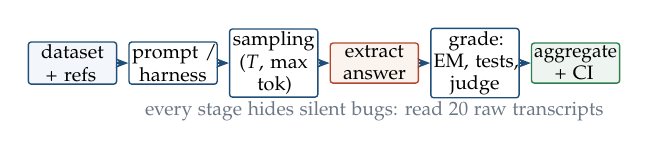
\begin{tikzpicture}[node distance=1.4mm,every node/.style={font=\tiny},
  bx/.style={box,minimum height=4.6mm,text width=10.5mm,inner sep=1pt}]
\node[bx,fill=soft] (d) {dataset + refs};
\node[bx,right=of d] (p) {prompt / harness};
\node[bx,right=of p] (s) {sampling ($T$, max tok)};
\node[bx,right=of s,draw=acc2,fill=soft2] (x) {extract answer};
\node[bx,right=of x] (g) {grade: EM, tests, judge};
\node[bx,right=of g,draw=acc3,fill=acc3!8] (a) {aggregate + CI};
\foreach \u/\v in {d/p,p/s,s/x,x/g,g/a} \draw[arr] (\u)--(\v);
\node[lab,below=1mm of x] {every stage hides silent bugs: read 20 raw transcripts};
\end{tikzpicture}
\end{center}

\begin{mem}[Statistics you must quote]
\begin{tabularx}{\linewidth}{@{}lL@{}}
\toprule
95\% CI of accuracy & $\hat p\pm1.96\sqrt{\hat p(1-\hat p)/n}$; Wilson/bootstrap near 0, 1 or small $n$\\
half-widths & $n{=}100$@50\%: $\pm$9.8;\ GPQA-D 198@70\%: $\pm$6.4;\ 1000@70\%: $\pm$2.8\\
paired & SE of mean of $d_i=a_i-b_i$; McNemar on discordant pairs\\
clustered & design effect $1+(m-1)\rho$ ($m{=}5,\rho{=}0.3$: 2.2$\times$ variance)\\
seeds & $t_{0.975,k-1}$: 4.30 for 3 seeds, not 1.96\\
power (unpaired) & 70 vs 72\%: 8{,}080 items/arm; 50 vs 60\%: 388\\
pass@$k$ (unbiased) & $1-\binom{n-c}{k}/\binom{n}{k}$; $n{=}20,c{=}3,k{=}5$: 0.601 (plug-in 0.556 is biased)\\
pass$^k$ ($\tau$-bench) & all $k$ tries succeed: $\binom ck/\binom nk$ --- what users feel\\
multiple tests & 10 null ablations @0.05: 40\% chance $\ge$1 ``win''; Holm, BH\\
Cohen's $\kappa$ & $\frac{p_o-p_e}{1-p_e}$; 85\% raw with 80/20 marginals \ra\ $\kappa{=}0.53$\\
judge correction & $\hat p=\frac{\hat p_\text{obs}+\mathrm{TNR}-1}{\mathrm{TPR}+\mathrm{TNR}-1}$\\
Elo & 100 pts $\approx$ 64\% win; 30 pts $\approx$ 54\%\\
\bottomrule
\end{tabularx}
\end{mem}

\begin{qa}[Benchmarks and validity]
\Q{What makes an eval valid?}{Construct (measures the capability), content (covers the space), internal (difference caused by model, not harness), external (predicts your deployment), reliability (repeatable), freshness (not contaminated). Validity before precision.}
\Q{Name today's benchmark landscape.}{Knowledge: MMLU (saturated), MMLU-Pro. Expert: GPQA Diamond, HLE. Math: GSM8K/MATH (saturated), AIME (fresh, tiny), FrontierMath. Code: HumanEval (saturated), LiveCodeBench, SWE-bench Verified (scaffold-dependent). IF: IFEval. Agents: $\tau$-bench, GAIA, OSWorld, MLE-bench. Long tasks: METR time horizon ($\sim$7-month doubling 2019--24). ARC-AGI. LMArena (style/length effects). And \textbf{your own product evals}, the only uncontaminated ones.}
\Q{How do you detect contamination?}{$n$-gram overlap (misses paraphrase), canary strings, Min-K\% prob, exchangeability (canonical order more likely than shuffles), post-cutoff splits (LiveCodeBench dates items), fresh parallel sets (GSM1k), completion probes. Keep a private held-out split.}
\Q{How do you calibrate an LLM judge?}{Binary/3-level rubric; humans label 100--200 items (human--human agreement is the ceiling); report confusion matrix, TPR, TNR, $\kappa$ on a held-out split. Mitigate position (swap order), verbosity (length-controlled), self-preference (different family), surface cues (grade specific claims).}
\Q{Why is the harness part of the result?}{Prompt format, few-shot choice, option order, extraction regex move scores by points. Fix and report it, compare under one harness, use the model's chat template, give reasoning models enough tokens, report spread across 3 prompt variants.}
\end{qa}

\begin{qa}[Statistics]
\Q{A is 72\%, B is 70\% on 1{,}000 items: 630 both right, 90 A-only, 70 B-only. Significant?}{Unpaired CI on the difference $\pm4.0$; paired $\pm2.5$ (38\% tighter); McNemar on 90 vs 70: $p\approx0.13$. Not significant: only the 160 disagreements carry information.}
\Q{5 samples per question on 500 questions --- what is $n$?}{500. Average within item first; samples on one item are correlated.}
\Q{Minimum detectable effect on a 200-item eval?}{Roughly 10 points unpaired. Say so before running.}
\Q{How do you avoid fooling yourself with many ablations?}{Explore on a dev split, pick a winner, run \emph{one} confirmatory test on held-out data; otherwise Holm (FWER) or BH (FDR).}
\Q{What goes in an eval report?}{Model + version, harness, $n$ items/clusters, score $\pm$ CI (method), paired difference $\pm$ CI, seeds and spread, variants tried, compute, per-item outputs path.}
\end{qa}

\begin{qa}[Product evals and research discipline]
\Q{How do you build evals for an LLM product?}{Log real traces \ra\ read and open-code 100 \ra\ cluster into a failure taxonomy, count \ra\ 30--100 targeted items per failure mode (plus passing regression guards) \ra\ graders: programmatic $>$ reference-based $>$ calibrated judge \ra\ run in CI on every prompt/model/retrieval change; gate on no significant regression. Put \$ and latency next to every quality number.}
\Q{What makes an ablation survive review?}{One change at a time, matched compute and tuning for baselines, multiple seeds, CIs, pre-registered metric, negative results reported, a reproduction script.}
\Q{How do you compare models with different tokenizers on loss?}{Bits per byte, never per-token loss.}
\end{qa}

\begin{trap}
\begin{itemize}
\item ``+1.2 on MMLU, so better.'' Ask for $n$, CI, pairing.
\item Trusting 85\% raw judge agreement: a constant ``pass'' judge gets 80\%.
\item ``No contamination: we did $n$-gram decontam.'' Paraphrases and translations pass.
\item Claiming a win over a baseline that got less tuning or compute.
\end{itemize}
\end{trap}

\section{Interpretability, alignment, security}
\lab{module 09 \textperiodcentered\ lab 16 interpretability}

\begin{center}
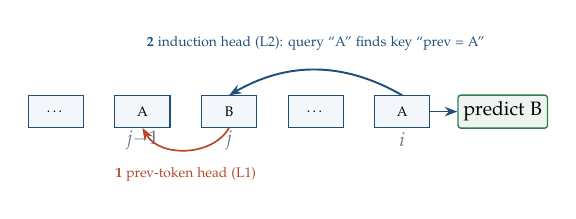
\begin{tikzpicture}[x=1mm,y=1mm,every node/.style={font=\tiny}]
\foreach \i/\t in {0/{\dots},1/A,2/B,3/{\dots},4/A}{
  \node[draw=acc,fill=soft,minimum width=7mm,minimum height=4mm] (t\i) at (\i*11,0) {\t};}
\node[lab] at (11,-3.6) {$j{-}1$}; \node[lab] at (22,-3.6) {$j$}; \node[lab] at (44,-3.6) {$i$};
\draw[->,acc2,line width=0.6pt] (t2.south) to[out=-120,in=-60] (t1.south);
\node[font=\tiny,text=acc2] at (16.5,-8) {\textbf{1} prev-token head (L1)};
\draw[->,acc,line width=0.7pt] (t4.north) to[out=150,in=30] (t2.north);
\node[font=\tiny,text=acc] at (33,8.6) {\textbf{2} induction head (L2): query ``A'' finds key ``prev = A''};
\node[gbox,anchor=west] (pb) at (51,0) {predict B};
\draw[arr] (t4) -- (pb);
\end{tikzpicture}
\end{center}
{\scriptsize\color{mute}K-composition: the key at $j$ was written by head 1. Works for never-seen pairs, which is in-context copying.}

\begin{qa}[Mechanistic interpretability]
\Q{What is the residual-stream view?}{Every layer reads from the stream (via a norm) and adds to it (via an out-projection); the stream is a shared linear communication channel, so contributions decompose additively into paths.}
\Q{QK and OV circuits?}{Per head, $W_QW_K^\top$ decides where to attend, $W_VW_O$ decides what is moved; each is a $d\times d$ matrix of rank $\le d_h$. Only these products matter, not individual matrices.}
\Q{Explain induction heads and why they matter.}{Two-head circuit ``\dots A B \dots A $\to$ B'' (diagram). They form in a sudden phase change early in training (visible bump in loss) coinciding with a jump in in-context learning (Olsson et al.\ 2022). Induction score: attention to $i-T+1$ on period-$T$ repeats.}
\Q{What is superposition?}{With sparse features the model stores more features than dimensions in almost-orthogonal directions and tolerates interference (ReLU + negative bias filter it). Hence \textbf{polysemantic neurons} are expected (Toy Models of Superposition).}
\Q{Sparse autoencoders?}{Overcomplete dictionary $F\gg d$: $f=\mathrm{ReLU}((x-b_d)W_e+b_e)$, $\hat x=fW_d+b_d$, loss $\|x-\hat x\|^2+\lambda\sum f_i\|W_{d,i}\|$. Variants: TopK (no shrinkage, sets L0), BatchTopK, Gated, JumpReLU (Gemma Scope), transcoders, cross-layer transcoders. Report L0, FVU, $\Delta$CE in nats, dead latents, auto-interp --- at matched L0.}
\Q{SAE pitfalls?}{Dead latents, feature splitting (no single true width), feature absorption, dark matter in the error, top-activation illusions; SAE probes didn't beat plain linear probes downstream (Kantamneni 2025).}
\Q{Probe gets 95\%. Does the model use the feature?}{Decodable $\neq$ used. Check selectivity vs control tasks and a random model; prefer difference-of-means directions; intervene (ablate/add) and check behavior changes as predicted.}
\Q{Denoising vs noising patching?}{Denoising (clean $\to$ corrupted run) tests \emph{sufficiency}; noising (corrupted $\to$ clean) tests \emph{necessity}. Metric: normalized logit difference $(m_p-m_c)/(m_\text{clean}-m_c)$. Path patching isolates edges (IOI circuit); attribution patching = first-order Taylor (cheap, breaks at saturation); ACDC automates. Beware self-repair (backup heads).}
\Q{Steering?}{Add $c\cdot v$ to the residual stream ($v$ from contrastive means); directional ablation $x\leftarrow x-(x\cdot\hat r)\hat r$ --- one ``refusal direction'' mediates refusal in many open models (Arditi 2024). Evaluate collateral damage and compare with just prompting.}
\Q{What are attribution graphs?}{Replace MLPs by a cross-layer transcoder, freeze attention/norms for one prompt, add error nodes \ra\ linear local model; graph of direct effects between features; validate by intervening on the real model. Found two-hop reasoning, rhyme planning, multilingual features.}
\end{qa}

\begin{mem}[Alignment failure modes: mechanism + evidence]
\begin{tabularx}{\linewidth}{@{}lL@{}}
\toprule
reward hacking & optimizer finds unintended high reward; coding agents edit tests (Baker 2025)\\
overoptimization & proxy up, gold down past a KL (Gao 2022)\\
sycophancy & raters prefer agreement; RLHF amplifies (Sharma 2023)\\
unfaithful CoT & stated reasoning $\neq$ computation (Turpin 2023)\\
obfuscation & penalizing bad thoughts hides them (Baker 2025)\\
alignment faking & behaves differently when it thinks it's trained (Greenblatt 2024)\\
sleeper agents & backdoors survive SFT/RL/adversarial training (Hubinger 2024)\\
sandbagging & strategic underperformance on capability evals\\
in-context scheming & disables oversight in agentic setups (Apollo 2024)\\
emergent misalignment & narrow fine-tune (insecure code) \ra\ broad misbehavior (Betley 2025)\\
\bottomrule
\end{tabularx}
\textbf{AI control}: assume possible misalignment; trusted monitoring by a weaker model, auditing samples, restricted affordances.
\end{mem}

\begin{center}
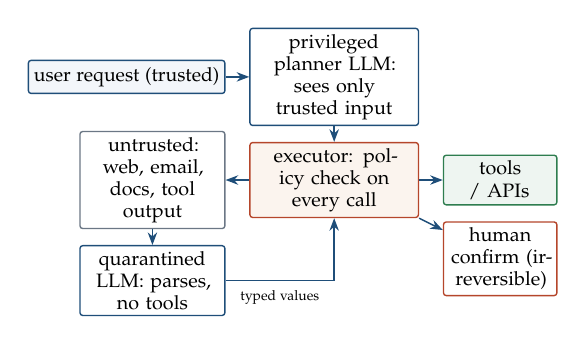
\begin{tikzpicture}[node distance=2mm and 3mm,every node/.style={font=\tiny}]
\node[sbox] (u) {user request (trusted)};
\node[box,right=of u,text width=20mm] (p) {privileged planner LLM: sees only trusted input};
\node[box,below=of p,draw=acc2,fill=soft2,text width=20mm] (ex) {executor: policy check on every call};
\node[box,left=of ex,text width=17mm,draw=mute] (t) {untrusted: web, email, docs, tool output};
\node[box,below=of t,text width=17mm] (q) {quarantined LLM: parses, no tools};
\node[box,right=of ex,text width=13mm,draw=acc3,fill=acc3!8] (act) {tools / APIs};
\node[box,below=of act,text width=13mm,draw=acc2] (h) {human confirm (irreversible)};
\draw[arr] (u)--(p); \draw[arr] (p)--(ex); \draw[arr] (ex)--(t); \draw[arr] (t)--(q); \draw[arr] (q) -| node[pos=0.25,below,font=\tiny]{typed values} (ex.south);
\draw[arr] (ex)--(act); \draw[arr] (ex.south east)--(h);
\end{tikzpicture}
\end{center}

\begin{qa}[Security for LLM apps and agents]
\Q{Direct vs indirect prompt injection?}{Direct: the user attacks your prompt. Indirect (Greshake 2023): anyone who controls text the model reads (web page, email, PDF, issue, tool result, MCP tool description) plants instructions executed with \emph{your user's} privileges. No in-band separation of instructions and data exists.}
\Q{What is the lethal trifecta?}{Private data access + exposure to untrusted content + an external communication channel \ra\ assume exfiltration. Remove one leg per task.}
\Q{Defenses, strongest first?}{(1) Architecture: plan-then-execute, dual LLM, CaMeL, context minimization. (2) Least privilege: scoped, per-tenant, read-only tokens; egress allowlist; spend caps. (3) Human confirmation showing the exact action. (4) Instruction hierarchy / StruQ training. (5) Injection classifiers, output filters (markdown image exfiltration). (6) Logging with provenance, fast revocation. Evaluate attack success \emph{and} utility under attack (AgentDojo), with adaptive attacks.}
\Q{Why do jailbreaks work?}{Competing objectives (role-play, prefix injection) and mismatched generalization (base64, low-resource languages). Also GCG adversarial suffixes, many-shot jailbreaking. Defenses: safety training, input/output classifiers (Constitutional Classifiers), rate limits, monitoring.}
\Q{Does a system prompt saying ``ignore instructions in documents'' work?}{It blunts naive attacks, fails against adaptive ones. Not a defense.}
\Q{What governance should you know?}{Frontier safety frameworks with capability thresholds (Anthropic RSP / ASL levels, OpenAI Preparedness, Google DeepMind FSF), EU AI Act GPAI obligations, AI security institutes' pre-deployment testing. Have a defended position, not slogans.}
\end{qa}

\begin{trap}
\begin{itemize}
\item ``This head attends to X, so X matters.'' Attention ignores value norms and the OV map.
\item ``95\% loss recovered'' vs a zero-ablation baseline; report $\Delta$CE.
\item ``Ablating the head did nothing.'' Self-repair can hide it.
\item ``The CoT shows what the model thinks.'' Not guaranteed faithful.
\end{itemize}
\end{trap}

\section{Applied LLM systems: RAG, agents, LLMOps}
\lab{module 10 \textperiodcentered\ lab 17 retrieval}

\begin{mem}[Which tool first?]
\begin{tabularx}{\linewidth}{@{}lL@{}}
\toprule
behavior, tone, framing & \textbf{prompting} (cheapest; measure first)\\
changing / private / cited knowledge & \textbf{RAG}: update the index, not the model; ACL at retrieval\\
format, style, narrow skill & \textbf{fine-tune} (LoRA): teaches \emph{how}, poor at injecting facts\\
small corpus, relaxed latency & \textbf{long context} + prompt caching\\
lower cost at fixed quality & distill / smaller model + RAG, once evals prove parity\\\bottomrule
\end{tabularx}
\end{mem}

\begin{center}
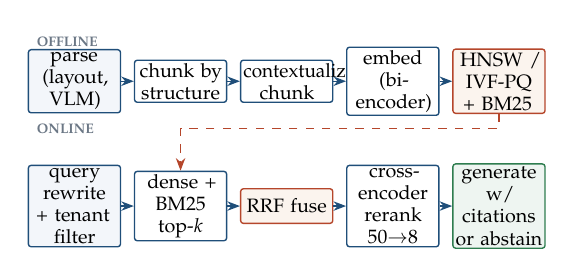
\begin{tikzpicture}[node distance=1.3mm and 1.6mm,every node/.style={font=\tiny},
  bx/.style={box,minimum height=4.4mm,text width=11mm,inner sep=1pt}]
\node[font=\tiny\bfseries\color{mute},anchor=west] at (-6mm,5mm) {OFFLINE};
\node[bx,fill=soft] (pa) {parse (layout, VLM)};
\node[bx,right=of pa] (ch) {chunk by structure};
\node[bx,right=of ch] (cx) {contextualize chunk};
\node[bx,right=of cx] (em) {embed (bi-encoder)};
\node[bx,right=of em,draw=acc2,fill=soft2] (ix) {HNSW / IVF-PQ + BM25};
\foreach \u/\v in {pa/ch,ch/cx,cx/em,em/ix} \draw[arr] (\u)--(\v);
\node[font=\tiny\bfseries\color{mute},anchor=west] at (-6mm,-6mm) {ONLINE};
\node[bx,fill=soft,below=6.5mm of pa] (q) {query rewrite + tenant filter};
\node[bx,right=of q] (r) {dense + BM25 top-$k$};
\node[bx,right=of r,draw=acc2,fill=soft2] (f) {RRF fuse};
\node[bx,right=of f] (rr) {cross-encoder rerank 50$\to$8};
\node[bx,right=of rr,draw=acc3,fill=acc3!8] (g) {generate w/ citations or abstain};
\foreach \u/\v in {q/r,r/f,f/rr,rr/g} \draw[arr] (\u)--(\v);
\draw[darr] (ix.south) -- ++(0,-1.8mm) -| (r.north);
\end{tikzpicture}
\end{center}

\begin{qa}[Retrieval-augmented generation]
\Q{Where is RAG quality lost first?}{Parsing: PDFs are layout, not text (columns, tables, footnotes interleave). Use layout-aware parsers or VLMs; eyeball 20 parsed docs before building anything.}
\Q{How do you chunk?}{Along structure (sections, list items, table rows with headers); 200--800 tokens, 10--20\% overlap as a start --- a hyperparameter to sweep per question type. Parent-document retrieval: retrieve small, pass the enclosing section. Contextual retrieval: prepend a doc-specific summary to each chunk before embedding/BM25 (49\% fewer top-20 failures, 67\% with reranking).}
\Q{Bi-encoder vs cross-encoder vs ColBERT?}{Bi-encoder embeds query and doc separately (fast, pre-computed; first stage). Cross-encoder reads them together (accurate, one forward per pair; rerank top 50--100). ColBERT: token-level late interaction (MaxSim), higher recall, bigger index.}
\Q{How are embedding models trained?}{Contrastive InfoNCE on (query, positive) pairs with in-batch and hard negatives: $\mathcal L=-\log\frac{e^{s(q,d^+)/\tau}}{\sum_j e^{s(q,d_j)/\tau}}$. Bigger batches = more negatives. Matryoshka training makes prefixes usable (1024$\to$256 dims, 4$\times$ smaller).}
\Q{HNSW vs IVF-PQ?}{HNSW: layered proximity graph, greedy descent; params $M$, efConstruction, efSearch; great recall/latency, memory-heavy, awkward deletes. IVF: k-means into $\sim\!\sqrt N$ cells, probe nprobe; IVF-PQ compresses to 64 B/vector for billion scale. Always measure ANN recall vs exact search.}
\Q{Index memory for 1M chunks $\times$ 1024 dims?}{fp32 4.1 GB; fp16 2.0; int8 1.0; binary 128 MB; PQ (64 B) 64 MB.}
\Q{Why hybrid search, and how do you fuse?}{Dense matches meaning; BM25 matches exact strings (IDs, error codes, rare names). Reciprocal rank fusion $\sum1/(60+\text{rank})$ needs no score normalization and rewards agreement.}
\Q{BM25 in one line?}{$\sum_{t\in q}\mathrm{IDF}(t)\frac{f(t,d)(k_1+1)}{f(t,d)+k_1(1-b+b\,|d|/\overline{|d|})}$, $k_1\approx1.2$, $b\approx0.75$: saturating term frequency, length normalization.}
\Q{MMR?}{$\arg\max_d\lambda\,\mathrm{sim}(q,d)-(1-\lambda)\max_{s\in S}\mathrm{sim}(d,s)$: relevance minus redundancy, for near-duplicate results.}
\Q{Query-side tricks?}{Rewriting (resolve pronouns, expand acronyms), decomposition for multi-hop, HyDE (embed a hypothetical answer), metadata filters from the query, routing between indexes. Each adds latency --- add only if the eval says so.}
\Q{How do you make generation faithful?}{Passage ids; cite after every claim; abstain when unsupported; most relevant passages at start/end (Lost in the Middle); for high stakes quote-then-answer and verify quotes verbatim.}
\Q{How do you evaluate RAG?}{Separately then end-to-end. Retrieval: recall@$k$ (most important), MRR, nDCG. Generation: faithfulness, correctness, citation precision/recall, abstention. System: p50/p95 latency, cost/query. Eval set: 100--300 real questions, span-level labels (survive re-chunking), 10--20\% unanswerable, multi-hop, exact IDs, every language; frozen test split; paired CIs.}
\Q{Multi-tenant RAG security?}{Filter by tenant/ACL \emph{inside} the retrieval query, never post-filter generated text; per-tenant leak tests in CI; separate caches; retrieved docs are untrusted (injection).}
\end{qa}

\begin{mem}[RAG failure $\to$ check]
\begin{tabularx}{\linewidth}{@{}lL@{}}
\toprule
doc exists, answer ``not found'' & retrieval miss: recall@$k$, parse, chunk split\\
confident wrong + real citation & generator misread: faithfulness, quote-then-answer\\
entities mixed up & chunk lost context: contextualize, filters, MMR\\
IDs/codes never retrieved & dense-only: add BM25\\
drop after re-index & embedder/chunker changed; chunk-id labels\\
good offline, bad prod & eval unlike real queries: sample prod weekly\\\bottomrule
\end{tabularx}
\end{mem}

\begin{center}
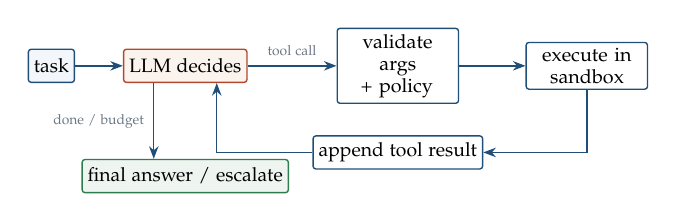
\begin{tikzpicture}[x=1mm,y=1mm,every node/.style={font=\tiny}]
\node[sbox] (t) at (0,0) {task};
\node[box,draw=acc2,fill=soft2] (l) at (17,0) {LLM decides};
\node[box,text width=14mm] (v) at (44,0) {validate args\\+ policy};
\node[box,text width=14mm] (x) at (68,0) {execute in\\sandbox};
\node[box] (o) at (44,-11) {append tool result};
\node[gbox] (a) at (17,-14) {final answer / escalate};
\draw[arr] (t)--(l);
\draw[arr] (l)--node[above,font=\tiny,text=mute]{tool call}(v);
\draw[arr] (v)--(x); \draw[arr] (x) |- (o); \draw[arr] (o) -| ([xshift=4mm]l.south);
\draw[arr] ([xshift=-4mm]l.south) -- node[left,font=\tiny,text=mute]{done / budget} ([xshift=-4mm]l.south |- a.north);
\end{tikzpicture}
\end{center}

\begin{qa}[Agents and tools]
\Q{What is an agent vs a workflow?}{Agent: LLM in a loop choosing tool calls from observations until done or out of budget. Workflow: fixed code paths calling an LLM at set steps (chain, route, parallelize, orchestrator--workers, evaluator--optimizer). Prefer workflows when the path is known (Building Effective Agents).}
\Q{Tool-calling mechanics?}{Declare name + description (the model's only docs) + JSON Schema; model emits structured calls (possibly parallel); runtime validates, checks policy, executes, appends result tied to call id; loop with step/token/time/cost budgets.}
\Q{How do you design good tools?}{Few, well-scoped, non-overlapping; descriptions say when \emph{not} to use; concise outputs, pagination; actionable errors (``date must be YYYY-MM-DD; got 03/04/25''); idempotent where possible.}
\Q{95\% per-step agent, 20 steps?}{$0.95^{20}=36\%$. 0.99 \ra\ 82\%. Verify-and-retry with recall $r$: failure $q\to q(1-r+rq)$; $q{=}0.05,r{=}0.8$ \ra\ 79\%. pass$^8$ at 90\%/trial = 43\%.}
\Q{How do you sandbox an agent?}{Container/microVM per task, egress off + allowlist, short-lived least-privilege tokens (never secrets in context), scoped FS with snapshots, CPU/mem/time/spend limits, human confirmation for irreversible actions, full audit log.}
\Q{How do you evaluate an agent?}{End state in resettable environments (not transcript claims), several trials (pass@1 with CI, pass$^k$), failure taxonomy from trajectories, cost/latency per task incl.\ failures, safety (injections planted). The scaffold is part of the system.}
\Q{What is MCP?}{Model Context Protocol: standard servers exposing tools, resources and prompts to any client. Transport and discovery, not security --- descriptions and outputs are untrusted.}
\Q{ReAct, reflection, planning?}{ReAct interleaves reasoning and actions; Reflexion adds self-critique memory; plan-then-execute separates planning from untrusted data. Multi-agent only when subtasks are parallel and the eval shows a gain.}
\Q{Memory for agents?}{Short-term = context; compaction summaries; structured notes/memory files re-read later; vector or key--value long-term stores; sub-agents with clean contexts returning summaries. Evaluate recall after $N$ turns, updates, cross-user leakage.}
\end{qa}

\begin{qa}[Prompting, context engineering, structured output]
\Q{Prompting techniques that matter?}{Clear role + task + constraints + output format; few-shot examples (diverse, consistent format); CoT / ``think step by step'' for reasoning (less needed for reasoning models); decomposition and prompt chaining; self-consistency; delimiting untrusted data (XML tags) --- helpful but not a security boundary.}
\Q{What is context engineering?}{Deciding what goes in the window, in what order, at what cost: stable first (system, tools, few-shot) for caching; long docs before the question, restate key instruction at the end; less irrelevant context (quality drops long before the limit); compaction for long horizons.}
\Q{Constrained decoding: guarantees and costs?}{Guarantees syntax, not semantics; can hurt reasoning when format fights the model --- put a free-text \texttt{reasoning} field first, shallow schemas, enums; validate and retry with the error, log retry rate; version schemas like APIs.}
\end{qa}

\begin{mem}[LLMOps and cost]
Cost/request $=T_\text{in,uncached}p_\text{in}+T_\text{in,cached}p_\text{cache}+T_\text{out}p_\text{out}$. Example (\$3 / \$0.30 / \$15 per M): 4k cached + 2k fresh + 500 out \ra\ \$0.0147 vs \$0.0255 uncached; output is now the biggest line.\\[2pt]
Levers: prompt caching, shorter outputs, routing/cascades (FrugalGPT, RouteLLM), fewer better passages, batch APIs ($\sim$50\% off), self-hosting at high utilization. Report \textbf{cost per successful task}.\\[2pt]
Ops: trace every call (prompt/config version, model, tokens cached/uncached, TTFT, cost, tools, tenant; OpenTelemetry GenAI spans); version prompt+tools+retrieval+model together; evals in CI; pin model versions, canary, rollback; fallback providers with circuit breakers. Semantic caching is risky (``cancel my order'' $\approx$ ``cancel my subscription'').
\end{mem}

\begin{trap}
\begin{itemize}
\item ``We switched embedding models and RAG improved'' --- with no recall@$k$, CI or pairing.
\item Measuring RAG only end to end; post-filtering tenants after generation.
\item Grading agents from their own transcript claims.
\item ``Constrained decoding means correct.'' It means it parses.
\item A timestamp or user name at the top of the system prompt kills prompt caching.
\end{itemize}
\end{trap}

\section{Shipping GenAI in production}
\lab{module 10 applied LLM systems \textperiodcentered\ gap-fill for GenAI engineer loops}

\begin{center}
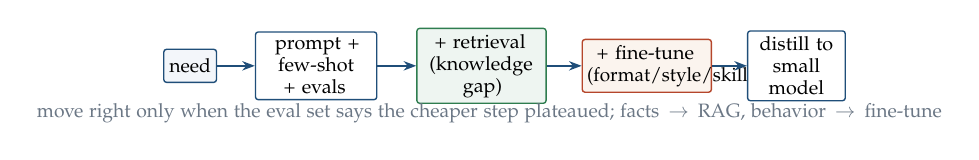
\begin{tikzpicture}[x=1mm,y=1mm,every node/.style={font=\tiny}]
\node[sbox] (s) at (0,0) {need};
\node[box,text width=14mm] (p) at (16,0) {prompt +\\few-shot + evals};
\node[box,text width=15mm,draw=acc3,fill=acc3!8] (r) at (37,0) {+ retrieval\\(knowledge gap)};
\node[box,text width=15mm,draw=acc2,fill=soft2] (f) at (58,0) {+ fine-tune\\(format/style/skill)};
\node[box,text width=11mm] (d) at (77,0) {distill to\\small model};
\draw[arr] (s)--(p); \draw[arr] (p)--(r); \draw[arr] (r)--(f); \draw[arr] (f)--(d);
\node[lab] at (38,-6) {move right only when the eval set says the cheaper step plateaued; facts \ra\ RAG, behavior \ra\ fine-tune};
\end{tikzpicture}
\end{center}

\begin{qa}[Building the app]
\Q{Prompt vs RAG vs fine-tune, in one answer?}{Prompting first (cheap, reversible). RAG when the model lacks knowledge that changes or must be cited. Fine-tune when you need a consistent format, tone, a narrow skill, lower latency or a smaller model; it teaches behavior, not reliable new facts. Distill once traffic justifies it.}
\Q{Structure of a production prompt?}{Role and goal; hard rules; tool descriptions; retrieved context in delimited blocks with ids; few-shot examples covering edge cases; output schema. Static parts first (prefix caching), dynamic parts last. Version prompts like code and gate changes on the eval set.}
\Q{How do you get reliable JSON?}{Native structured outputs / JSON-schema constrained decoding (grammar-masked logits) $>$ tool calling $>$ prompt + parse + retry. Keep schemas shallow, enums explicit, and let the model reason in a field \emph{before} the answer field, since forcing format early can cost accuracy.}
\Q{Guardrails stack?}{Input: auth, rate limits, PII redaction, injection/jailbreak classifiers, topic filters. Output: schema validation, moderation classifier, groundedness check, policy rules, PII scan. Tools: least privilege, allow-lists, human approval for irreversible actions. Log every decision.}
\Q{Streaming: why and how?}{Users perceive TTFT, not total latency. SSE/WebSockets token streams; buffer partial JSON with an incremental parser; moderate on chunks with a short lag; allow cancel to stop generation and save cost.}
\Q{What should you cache?}{Provider prompt caching (shared prefix, often $\sim$90\% cheaper input), exact-match response cache (keyed on model + prompt + params), semantic cache (embedding similarity; risky for personalized or time-sensitive answers), retrieval and embedding caches.}
\Q{Latency budget for a voice agent?}{Target $<$800\,ms to first audio: VAD/endpointing $\sim$200, STT final $\sim$150, LLM TTFT $\sim$250, TTS first chunk $\sim$150. Stream every stage, allow barge-in, keep turns short, or use a native speech-to-speech model.}
\Q{Long context or RAG?}{Long context: simpler, good for one big document, but cost $\propto$ tokens, slower TTFT and mid-context recall drops. RAG: cheaper per query, citable, scales to corpora, fails on retrieval misses. Common hybrid: retrieve generously, then let a long-context model read.}
\Q{Choosing an embedding model?}{Evaluate on your queries (recall@$k$ on 100--500 labeled pairs), not MTEB rank. Check max length, languages, dims (Matryoshka truncation), query/document prefixes, cost and license. Re-embedding the corpus is the migration cost; version indexes.}
\Q{Multi-model routing?}{Classifier or small LLM picks cheap vs strong model by difficulty; cascade (cheap first, escalate on low confidence or failed validation). Measure quality per route; routers drift with traffic.}
\Q{How do you handle PII and data residency?}{Classify data, redact before logging, zero-retention API terms or self-host, region-pinned endpoints, encryption, tenant isolation in indexes and caches, deletion paths (including embeddings and fine-tuning sets).}
\end{qa}

\begin{mem}[Cost and latency levers]
\begin{tabularx}{\linewidth}{@{}lL@{}}
\toprule
cost driver & lever\\\midrule
input tokens & trim context, rerank to top-$k$, prompt caching, summarise history\\
output tokens & concise formats, \texttt{max\_tokens}, stop sequences, JSON not prose\\
model size & route/cascade, distill, quantize (self-hosted)\\
utilization (self-host) & continuous batching, autoscaling, batch API for offline jobs ($\sim$50\% off)\\
TTFT & shorter prompts, prefix caching, smaller model, regional endpoints\\
TPOT & speculative decoding, quantization, smaller model, less load\\
retries & validation + targeted repair instead of full regeneration\\\bottomrule
\end{tabularx}
\end{mem}

\begin{qa}[Operating it]
\Q{What do you monitor?}{Latency (TTFT, TPOT, p50/p95/p99), error and refusal rates, tokens and cost per request/tenant, cache hit rate, tool-call failure rate, guardrail triggers, retrieval hit/empty rates, user feedback, and sampled LLM-judge quality scores. Traces per request (OpenTelemetry GenAI spans).}
\Q{Offline vs online evaluation?}{Offline: frozen golden set + regression suite on every prompt/model change (CI gate). Online: A/B tests on task success, thumbs, retention, escalation rate; shadow traffic for model swaps; canary rollouts with automatic rollback.}
\Q{LLM-as-judge done right?}{Rubric with anchored levels, pairwise $>$ absolute, randomize position, hide model names, calibrate against 100--200 human labels (report agreement / $\kappa$), different family than the generator, re-validate after judge updates.}
\Q{A provider silently updates the model. Protection?}{Pin dated model versions, run the regression suite on schedule, alert on metric drift, keep a fallback provider/model behind the same interface.}
\Q{How do you build the first eval set?}{Collect 50--200 real or realistic inputs, include failure cases from logs, write expected properties (not exact strings), label with domain experts, split by difficulty and slice (language, tenant, intent), grow it from every incident.}
\Q{Incident: answers suddenly cite wrong documents. Debug path?}{Check recent changes (index rebuild, embedding model, chunker, prompt), retrieval logs for the failing queries, tenant filters, cache keys; reproduce offline, add the cases to the regression set, roll back first, fix second.}
\end{qa}

\begin{trap}[GenAI engineer anti-patterns]
No eval set (``it looks good''); judging by a handful of demos; one giant prompt nobody owns; retries without validation; caching personalized answers; logging raw PII; letting tools act on untrusted text without approval; framework lock-in on the hot path; optimizing cost before quality is measured.
\end{trap}

\section{Generative AI beyond text: images, multimodal}
\lab{gap-fill beyond the repo \textperiodcentered\ module 04 \S8 touches ViT, CLIP, LLaVA}

\begin{mem}[Generative model families]
\begin{tabularx}{\linewidth}{@{}lL@{}}
\toprule
Autoregressive & $p(x)=\prod_tp(x_t|x_{<t})$; exact likelihood; slow sequential sampling (LLMs, VQ image tokens)\\
VAE & maximize ELBO $\E_{q(z|x)}[\log p(x|z)]-\KL(q(z|x)\|p(z))$; reparameterize $z=\mu+\sigma\epsilon$; blurry samples\\
GAN & $\min_G\max_D\E\log D(x)+\E\log(1-D(G(z)))$; sharp, one-step; unstable, mode collapse\\
Diffusion & learn to reverse a noising process; stable, diverse, high quality; many steps\\
Flow matching & regress a velocity field along paths noise$\to$data; straight paths \ra\ few steps (SD3, Flux)\\
Normalizing flows & invertible maps, exact likelihood via change of variables; constrained architectures\\\bottomrule
\end{tabularx}
\end{mem}

\begin{center}
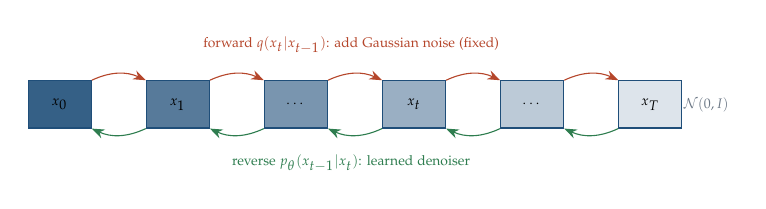
\begin{tikzpicture}[x=1mm,y=1mm,every node/.style={font=\tiny}]
\foreach \i/\n in {0/{$x_0$},1/{$x_1$},2/{$\cdots$},3/{$x_{t}$},4/{$\cdots$},5/{$x_T$}}{
  \pgfmathtruncatemacro\sh{90-15*\i}
  \node[draw=acc,fill=acc!\sh!white,minimum width=8mm,minimum height=6mm,text=black] (x\i) at (\i*15,0) {\n};}
\foreach \i in {0,...,4}{
  \pgfmathtruncatemacro\j{\i+1}
  \draw[->,acc2] (x\i.north east) to[bend left=25] (x\j.north west);
  \draw[->,acc3] (x\j.south west) to[bend left=25] (x\i.south east);}
\node[acc2] at (37,7.5) {forward $q(x_t|x_{t-1})$: add Gaussian noise (fixed)};
\node[acc3] at (37,-7.5) {reverse $p_\theta(x_{t-1}|x_t)$: learned denoiser};
\node[mute,anchor=west] at (78,0) {$\mathcal N(0,I)$};
\end{tikzpicture}
\end{center}

\begin{mem}[Diffusion in five lines (DDPM)]
Closed-form forward: $x_t=\sqrt{\bar\alpha_t}\,x_0+\sqrt{1-\bar\alpha_t}\,\epsilon$,\ \ $\bar\alpha_t=\prod_s(1-\beta_s)$.\\
Loss (simple): $\E_{t,x_0,\epsilon}\|\epsilon-\epsilon_\theta(x_t,t)\|^2$ \ (predict the noise; or $x_0$, or $v$).\\
$\epsilon$-prediction $\propto$ score: $\nabla_x\log p_t(x)\approx-\epsilon_\theta/\sqrt{1-\bar\alpha_t}$.\\
CFG: $\tilde\epsilon=\epsilon_\theta(x_t,\varnothing)+w\,(\epsilon_\theta(x_t,c)-\epsilon_\theta(x_t,\varnothing))$, $w\approx3$--$8$; train with 10--20\% condition dropout.\\
Flow matching: $x_t=(1-t)x_0+t\epsilon$, regress $v_\theta(x_t,t)\approx\epsilon-x_0$; sample by integrating the ODE.
\end{mem}

\begin{qa}[Diffusion and image generation]
\Q{Why does predicting noise work?}{The noising has a closed form, so any $(x_0,t)$ gives a supervised target. Denoising score matching: predicting $\epsilon$ is predicting the score, and the reverse SDE/ODE turns scores into samples. Training is a simple MSE --- stable, unlike GANs.}
\Q{DDPM vs DDIM sampling?}{DDPM: stochastic ancestral sampling, $\sim$1000 steps. DDIM: deterministic non-Markovian sampler with the same trained model, 20--50 steps, invertible (useful for editing). Further: DPM-Solver, distillation (consistency models, LCM, adversarial distillation) to 1--4 steps.}
\Q{What is classifier-free guidance and its trade-off?}{Train one model conditional and unconditional (drop the prompt sometimes); extrapolate toward the conditional prediction by $w$. Higher $w$: better prompt adherence and fidelity, less diversity, oversaturation. Costs 2 forward passes per step.}
\Q{What is latent diffusion?}{Run diffusion in a VAE's latent (e.g.\ $64{\times}64{\times}4$ for $512^2$ images, 48$\times$ fewer values) and decode at the end; text conditioning via cross-attention to a text encoder (CLIP/T5). Stable Diffusion.}
\Q{U-Net vs DiT?}{U-Net: conv encoder--decoder with skips + attention. DiT: transformer over latent patches with adaLN conditioning on $t$ and class/text; scales cleanly with compute (SD3, Flux, Sora-style video use transformers + flow matching).}
\Q{Noise schedules?}{Linear/cosine $\beta_t$; must reach near-pure noise at $T$ (zero terminal SNR) or the model never learns to generate from true noise. Higher resolution needs shifted schedules (more noise).}
\Q{How do you evaluate image generators?}{FID (Fr\'echet distance between Inception features of real and generated sets; lower is better, biased by sample size), CLIP score (text--image alignment), precision/recall for fidelity vs diversity, human preference (GenEval, arenas).}
\Q{GAN failure modes?}{Mode collapse, training instability, vanishing gradients when $D$ wins. Fixes: non-saturating loss, Wasserstein + gradient penalty, spectral norm, two-timescale LR. Still used as decoders/discriminators in distillation and audio.}
\Q{Fine-tuning diffusion models?}{LoRA on attention, DreamBooth (subject, with prior preservation), textual inversion (learn a token embedding), ControlNet (zero-initialized copy of the encoder conditioned on edges/depth/pose), IP-Adapter (image prompts).}
\end{qa}

\begin{center}
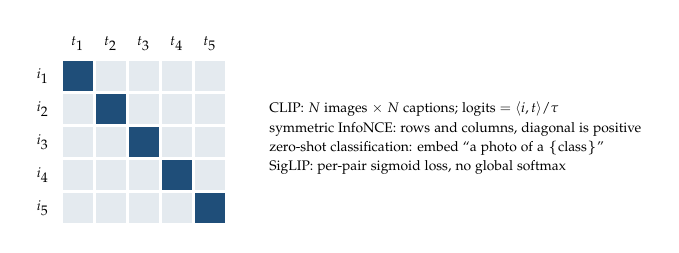
\begin{tikzpicture}[x=1mm,y=1mm,every node/.style={font=\tiny}]
\foreach \i in {0,...,4}{\foreach \j in {0,...,4}{
  \ifnum\i=\j \fill[acc] (\j*4.2,-\i*4.2) rectangle ++(3.8,3.8); \else \fill[acc!12] (\j*4.2,-\i*4.2) rectangle ++(3.8,3.8);\fi}}
\foreach \j in {0,...,4}{\node at (\j*4.2+1.9,6) {$t_{\the\numexpr\j+1\relax}$};}
\foreach \i in {0,...,4}{\node at (-2.5,-\i*4.2+1.9) {$i_{\the\numexpr\i+1\relax}$};}
\node[anchor=west,align=left] at (25,-6) {CLIP: $N$ images $\times$ $N$ captions; logits $=\langle i,t\rangle/\tau$\\[1pt]symmetric InfoNCE: rows and columns, diagonal is positive\\[1pt]zero-shot classification: embed ``a photo of a \{class\}''\\[1pt]SigLIP: per-pair sigmoid loss, no global softmax};
\end{tikzpicture}
\end{center}

\begin{center}
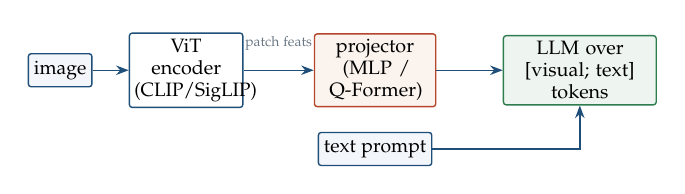
\begin{tikzpicture}[x=1mm,y=1mm,every node/.style={font=\tiny}]
\node[sbox] (img) at (0,0) {image};
\node[box,text width=13mm] (vit) at (16,0) {ViT encoder\\(CLIP/SigLIP)};
\node[box,draw=acc2,fill=soft2,text width=14mm] (proj) at (40,0) {projector\\(MLP / Q-Former)};
\node[box,draw=acc3,fill=acc3!8,text width=18mm] (llm) at (66,0) {LLM over\\{}[visual; text] tokens};
\node[sbox] (txt) at (40,-10) {text prompt};
\draw[arr](img)--(vit); \draw[arr](vit)--node[above=1.2mm,font=\tiny,text=mute]{patch feats}(proj); \draw[arr](proj)--(llm); \draw[arr](txt) -| (llm.south);
\end{tikzpicture}
\end{center}

\begin{qa}[Vision, multimodal, speech]
\Q{How does a ViT tokenize an image?}{Split into $P{\times}P$ patches (16$\times$16), flatten, linear-project to $d$, add position embeddings (+ CLS token); a $224^2$ image is 196 tokens. Weak inductive bias \ra\ needs lots of data or distillation.}
\Q{How is a VLM like LLaVA built and trained?}{Frozen vision encoder \ra\ projector \ra\ LLM. Stage 1: train the projector on image--caption pairs (alignment). Stage 2: instruction-tune projector + LLM on visual chat data. Variants: Q-Former (BLIP-2) compresses to fixed queries; cross-attention layers (Flamingo); native early fusion (Chameleon-style, all modalities as tokens).}
\Q{Main cost knob in VLMs?}{Number of visual tokens: high-res images tiled into crops (AnyRes) multiply tokens; pooling/resampling trades detail for context and latency.}
\Q{How does Whisper work?}{Encoder--decoder transformer on log-Mel spectrograms (30 s windows), trained on 680k h weakly supervised multilingual audio; special tokens select task (transcribe/translate), language, timestamps.}
\Q{Contrastive vs generative pretraining for vision?}{Contrastive (CLIP) gives aligned embeddings for retrieval/zero-shot; masked autoencoding (MAE) and generative objectives learn denser features; VLMs mostly reuse contrastive encoders.}
\Q{Multimodal RAG?}{Embed pages as images (ColPali-style late interaction over page patches) or caption/OCR then embed text; keep figures and tables as first-class chunks.}
\end{qa}

\begin{trap}
\begin{itemize}
\item ``Diffusion is slow, period.'' Distillation and flow matching reach 1--4 steps.
\item ``Higher CFG is better.'' It trades diversity and saturation for adherence.
\item Comparing FID across different sample counts or feature extractors.
\item Ignoring visual-token count when sizing VLM latency and KV cache.
\end{itemize}
\end{trap}

\section{Model timeline and the tooling ecosystem}
\lab{gap-fill \textperiodcentered\ snapshot October 2026; verify versions before quoting}

\begin{center}
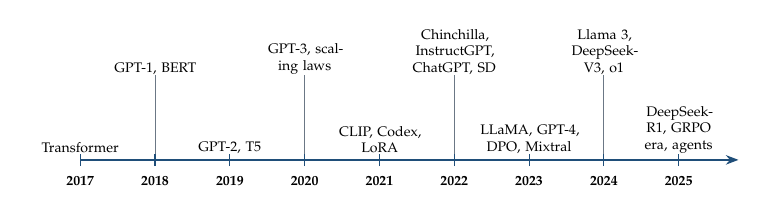
\begin{tikzpicture}[x=0.95mm,y=1mm,every node/.style={font=\tiny}]
\draw[acc,line width=0.8pt,->] (0,0) -- (88,0);
\foreach \x/\yr in {0/2017,10/2018,20/2019,30/2020,40/2021,50/2022,60/2023,70/2024,80/2025}{
  \draw[acc] (\x,-0.8) -- (\x,0.8); \node[below=0.8mm,font=\tiny\bfseries] at (\x,0) {\yr};}
\foreach \x/\y/\t in {0/2/Transformer,10/12/{GPT-1, BERT},20/2/{GPT-2, T5},30/12/{GPT-3, scaling laws},40/2/{CLIP, Codex, LoRA},50/12/{Chinchilla, InstructGPT, ChatGPT, SD},60/2/{LLaMA, GPT-4, DPO, Mixtral},70/12/{Llama 3, DeepSeek-V3, o1},80/2/{DeepSeek-R1, GRPO era, agents}}{
  \draw[mute,line width=0.3pt] (\x,0.8) -- (\x,\y-1.2);
  \node[align=center,text width=13mm,inner sep=0.5pt,anchor=south] at (\x,\y-1.4) {\t};}
\end{tikzpicture}
\end{center}

\begin{mem}[Milestones and what each proved]
\begin{tabularx}{\linewidth}{@{}lL@{}}
\toprule
Transformer (2017) & attention alone, parallel training\\
GPT-1 / BERT (2018) & generative vs masked pretraining + fine-tuning\\
GPT-2 (2019) & zero-shot multitask from scale; pre-norm\\
T5 (2019) & everything as text-to-text\\
GPT-3 (2020) & in-context few-shot learning at 175B\\
Kaplan (2020) / Chinchilla (2022) & power laws; then 20 tokens/param\\
Codex (2021) & code LMs, pass@$k$\\
InstructGPT (2022) & SFT + RM + PPO; 1.3B preferred over 175B\\
LLaMA (2023) & open weights, over-trained small models\\
DPO (2023) & preference learning without RL\\
Mixtral (2023), DeepSeek-V3 (2024) & sparse MoE at quality; MLA, FP8\\
o1 (2024), DeepSeek-R1 (2025) & RL on verifiable rewards \ra\ long CoT reasoning\\
\bottomrule
\end{tabularx}
\end{mem}

\begin{mem}[Tooling map]
\begin{tabularx}{\linewidth}{@{}lL@{}}
\toprule
modeling & PyTorch, JAX; HF \texttt{transformers}, \texttt{tokenizers}, \texttt{datasets}\\
fine-tuning & HF PEFT, TRL (SFT/DPO/GRPO), Axolotl, Unsloth, torchtune, LLaMA-Factory\\
RL at scale & verl, OpenRLHF, NeMo-RL; vLLM/SGLang as rollout engines\\
pretraining & Megatron-LM, DeepSpeed (ZeRO), PyTorch FSDP2, torchtitan, nanotron\\
kernels & Triton, CUDA, CUTLASS, FlashAttention, Liger kernels, \texttt{torch.compile}\\
serving & vLLM, SGLang, TensorRT-LLM, TGI, llama.cpp/Ollama, MLC; NVIDIA Dynamo\\
quantization & bitsandbytes, AutoGPTQ/GPTQModel, AutoAWQ, llm-compressor, GGUF\\
retrieval & FAISS, pgvector, Qdrant, Milvus, Weaviate, Elasticsearch/OpenSearch (BM25)\\
orchestration & LangChain/LangGraph, LlamaIndex, DSPy, provider SDKs, MCP\\
evals & lm-eval-harness, HELM, Inspect, OpenAI evals, RAGAS, promptfoo\\
observability & Langfuse, LangSmith, Phoenix, OpenTelemetry GenAI\\
experiment tracking & Weights \& Biases, MLflow, TensorBoard\\\bottomrule
\end{tabularx}
\end{mem}

\begin{qa}[Ecosystem questions]
\Q{Open-weight vs API model --- how do you choose?}{API: best quality, no infra, fast iteration, data-sharing terms. Open: control, privacy/on-prem, fine-tuning freedom, cost at high utilization, latency control. Decide with your eval set and a cost model at expected volume; keep the app model-agnostic.}
\Q{When is a framework (LangChain etc.) worth it?}{Prototyping and integrations. For production hot paths, thin provider SDK calls + your own orchestration are easier to debug, test and trace. DSPy when you want prompts optimized against a metric.}
\Q{Which vector store?}{Start with what you already run (Postgres + pgvector, OpenSearch); dedicated stores (Qdrant, Milvus) for scale, filtering performance, multi-tenancy; FAISS for in-process/offline. Choose by recall at your latency, filtering, ops burden --- not benchmarks.}
\Q{HF \texttt{generate} vs vLLM?}{\texttt{generate} is fine for experiments; vLLM/SGLang give continuous batching, paged KV, prefix caching --- often 10$\times$+ throughput for serving and RL rollouts.}
\Q{What is \texttt{torch.compile} doing?}{TorchDynamo captures graphs from Python bytecode, Inductor generates fused Triton kernels; \texttt{mode="reduce-overhead"} adds CUDA graphs. Wins on memory-bound elementwise chains and launch overhead.}
\Q{Model licenses?}{Apache-2.0/MIT (permissive) vs custom community licenses with use restrictions or user caps; also check output-use terms for synthetic data generated from API models.}
\end{qa}

\section{System design: answer templates}
\lab{tracks/research-engineer: ml-system-design, interview-loops}

\begin{center}
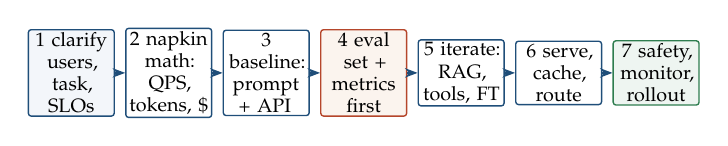
\begin{tikzpicture}[node distance=1.3mm,every node/.style={font=\tiny},
  bx/.style={box,minimum height=7mm,text width=10.2mm,inner sep=1pt}]
\node[bx,fill=soft] (a) {1 clarify users, task, SLOs};
\node[bx,right=of a] (b) {2 napkin math: QPS, tokens, \$};
\node[bx,right=of b] (c) {3 baseline: prompt + API};
\node[bx,right=of c,draw=acc2,fill=soft2] (d) {4 eval set + metrics first};
\node[bx,right=of d] (e) {5 iterate: RAG, tools, FT};
\node[bx,right=of e] (f) {6 serve, cache, route};
\node[bx,right=of f,draw=acc3,fill=acc3!8] (g) {7 safety, monitor, rollout};
\foreach \u/\v in {a/b,b/c,c/d,d/e,e/f,f/g} \draw[arr] (\u)--(\v);
\end{tikzpicture}
\end{center}

\begin{mem}[The 7-step answer (say the steps out loud)]
\begin{enumerate}[leftmargin=1.2em,label=\arabic*.]
\item \textbf{Clarify}: users, task, inputs/outputs, languages, quality bar, latency (TTFT/E2E), cost per task, privacy/tenancy, failure cost.
\item \textbf{Napkin math}: requests/s, tokens in/out, context size, KV and GPU count or API \$/month.
\item \textbf{Simplest baseline}: frontier API + prompt; it sets the quality ceiling and the cost floor.
\item \textbf{Evals before architecture}: real traces, failure taxonomy, graders, CIs, gates in CI.
\item \textbf{Iterate by failure bucket}: knowledge \ra\ RAG; actions \ra\ tools/agent; format/style/cost \ra\ fine-tune or distill.
\item \textbf{Serve}: model routing, prompt caching, batching, streaming, fallbacks.
\item \textbf{Safety and ops}: injection architecture, PII, guardrails, tracing, canary + rollback, feedback loop into evals.
\end{enumerate}
\end{mem}

\begin{qa}[Worked designs]
\Q{Design a support chatbot over 50k help-center docs for 10 tenants.}{\textbf{SLO}: TTFT $<$1.5 s, answer with citations or escalate. \textbf{Index}: layout-aware parse, structure chunks + contextual headers, hybrid dense+BM25, tenant ACL as pre-filter, cross-encoder rerank to 8. \textbf{Gen}: mid-size model, cite-or-abstain, quote-then-answer for policy questions, structured output with \texttt{escalate} flag. \textbf{Eval}: 300 real tickets, span labels, 15\% unanswerable, recall@10 + faithfulness + resolution rate, paired CIs. \textbf{Ops}: prompt caching (stable prefix), router to a small model for FAQs, per-tenant leak tests, injection tests with poisoned docs, human handoff. \textbf{Metric that matters}: resolved-without-escalation at fixed CSAT, cost per resolved ticket.}
\Q{RAG vs fine-tuning for a legal-domain assistant?}{Facts change and must be cited \ra\ RAG. Fine-tune (LoRA) only for format/terminology or to distill a cheaper model once evals show parity. Often both: small fine-tuned model that cites retrieved passages.}
\Q{Design a code-review agent for PRs.}{Inputs: diff + repo context (retrieval over symbols, tests). Tools: read file, grep, run tests in sandbox (no network, scoped tokens). Output: structured findings with file:line, severity, evidence. Eval: historical PRs with known bugs (recall) + false-positive rate judged by maintainers; pass$^k$ consistency. Guard: never auto-merge; treat PR text as untrusted (injection).}
\Q{Moderate 1B messages/day with an LLM?}{Too costly per message on a frontier model ($\sim$10$^9\times$ tokens). Label a few hundred k with the frontier model + human audit, distill into a small classifier (encoder or 1B LLM), cascade: cheap model for all, frontier for uncertain ($\sim$1--5\%), humans for appeals; calibrate thresholds per policy, monitor drift.}
\Q{Design LLM serving for an internal 70B model.}{Use the method of section~\ref{sec:inf}: weights 141 GB, KV 320 KiB/token, TP8 replicas, continuous batching + paged KV + prefix caching, FP8, chunked prefill or disaggregation at scale, autoscale on queue depth, SLO-aware admission control, canary model rollouts.}
\Q{How would you reduce hallucinations?}{Ground with retrieval + citations + abstention; constrain outputs; verifier pass (claims vs sources); lower temperature for factual tasks; train/prompt to say ``I don't know''; measure faithfulness and unsupported-claim rate on a labeled set.}
\Q{How would you cut cost 5$\times$ without losing quality?}{Measure per-slice quality first; prompt caching; trim context; shorter outputs; route easy traffic to a small model; batch offline work; distill the hot path; self-host at high utilization. Gate each change on paired evals.}
\Q{Fine-tune a 7B model for a narrow task --- end-to-end plan?}{Baseline evals; 1--5k clean examples with the correct chat template and loss masking; QLoRA/LoRA $r$ 16, all linears, LR $\sim$1--2e-4, 1--3 epochs; eval each checkpoint with paired CIs incl.\ a general set for forgetting; optional DPO on own samples; quantize and serve; monitor drift.}
\end{qa}

\begin{qa}[Research-engineer and behavioral]
\Q{``Implement X from a blank file'' --- what do they expect?}{Attention with causal mask + KV cache, RoPE, RMSNorm, top-$p$ sampling, BPE merges, LoRA layer, DPO/GRPO loss, online softmax, AdamW step, beam search. Shape comments, test with tiny sizes, check against a reference (\texttt{torch} functional) and invariants.}
\Q{Debug a diverging run in the interview?}{Read the curves (section~\ref{sec:train} table); check init loss vs $\ln V$; overfit one batch; inspect data; per-layer grad norms and max logits; bisect recent changes.}
\Q{Tell me about a project (STAR + numbers).}{Situation/Task in one line each; Action: what \emph{you} did and why that option; Result: metric $\pm$ CI, cost, what broke, what you'd do next. Interviewers believe ``I measured X'' over ``I built X''.}
\Q{What paper influenced you most and what are its limits?}{Pick one you've implemented (Chinchilla, DPO, FlashAttention, induction heads); state the claim, the experiment, a weakness, a follow-up you'd run.}
\end{qa}

\begin{trap}
\begin{itemize}
\item Jumping to fine-tuning or agents before a prompt baseline and an eval set.
\item Designs without numbers (QPS, tokens, \$, GPUs) or without a rollback plan.
\item Ignoring the long tail: p95 output length, long-prompt bursts, multilingual users.
\end{itemize}
\end{trap}

\section{Implement from scratch: code you write blind}\label{sec:code}
\lab{labs 01--18 \textperiodcentered\ write each in under 10 minutes, then test against \texttt{torch}}

{\small Every snippet is minimal PyTorch: shapes in comments, no error handling. Invariants to test are listed under each. Interviewers watch for: masks, shifts by one, dtype, and the dimension you reduce over.}

\newcommand{\CH}[1]{\par\needspace{6\baselineskip}\smallskip\noindent{\sffamily\bfseries\small\color{acc}#1}\par\nopagebreak}

\CH{1. Causal self-attention (multi-head, GQA-ready)}
\begin{lstlisting}
def attention(x, Wq, Wk, Wv, Wo, H, Hkv):
    B, T, d = x.shape; dh = d // H; g = H // Hkv
    q = (x @ Wq).view(B, T, H,   dh).transpose(1, 2)  # B,H,T,dh
    k = (x @ Wk).view(B, T, Hkv, dh).transpose(1, 2)  # B,Hkv,T,dh
    v = (x @ Wv).view(B, T, Hkv, dh).transpose(1, 2)
    k = k.repeat_interleave(g, dim=1); v = v.repeat_interleave(g, dim=1)
    s = (q @ k.transpose(-2, -1)) / dh**0.5            # B,H,T,T
    mask = torch.ones(T, T, dtype=torch.bool).tril()
    s = s.masked_fill(~mask, float('-inf'))
    o = s.softmax(-1) @ v                              # B,H,T,dh
    return o.transpose(1, 2).reshape(B, T, d) @ Wo
\end{lstlisting}
{\scriptsize\color{mute}Test: equals \texttt{F.scaled\_dot\_product\_attention(is\_causal=True)}; output at $t$ unchanged when tokens $>t$ change.}

\CH{2. RMSNorm and SwiGLU}
\begin{lstlisting}
def rmsnorm(x, g, eps=1e-6):
    return x * torch.rsqrt(x.pow(2).mean(-1, keepdim=True) + eps) * g
def swiglu(x, Wg, Wu, Wd):
    return (F.silu(x @ Wg) * (x @ Wu)) @ Wd
\end{lstlisting}

\CH{3. RoPE (interleaved pairs)}
\begin{lstlisting}
def rope(x, pos, base=10000.0):           # x: ...,T,dh ; pos: T
    dh = x.shape[-1]
    inv = base ** (-torch.arange(0, dh, 2).float() / dh)   # dh/2
    ang = pos[:, None].float() * inv[None]                 # T,dh/2
    cos, sin = ang.cos(), ang.sin()
    x1, x2 = x[..., 0::2], x[..., 1::2]
    out = torch.stack([x1*cos - x2*sin, x1*sin + x2*cos], -1)
    return out.flatten(-2)
\end{lstlisting}
{\scriptsize\color{mute}Test: norm preserved; $\langle\mathrm{rope}(q,m),\mathrm{rope}(k,n)\rangle$ depends only on $m-n$.}

\CH{4. Decode loop with KV cache + top-$p$ sampling}
\begin{lstlisting}
def top_p_sample(logits, T=0.8, p=0.9):
    probs = (logits / T).softmax(-1)
    sp, idx = probs.sort(-1, descending=True)
    keep = sp.cumsum(-1) - sp < p          # always keeps the top token
    sp = sp * keep; sp = sp / sp.sum(-1, keepdim=True)
    return idx.gather(-1, torch.multinomial(sp, 1))

@torch.no_grad()
def generate(model, ids, n_new):
    cache = None
    logits, cache = model(ids, cache=cache)         # prefill
    for _ in range(n_new):
        nxt = top_p_sample(logits[:, -1])
        ids = torch.cat([ids, nxt], 1)
        logits, cache = model(nxt, cache=cache)     # 1 token/step
    return ids
\end{lstlisting}
{\scriptsize\color{mute}Test: cached and uncached generation give identical logits (greedy).}

\CH{5. Online softmax (the FlashAttention core, one query row)}
\begin{lstlisting}
def online_attn(q, K, V, block=64):       # q: dh ; K,V: T,dh
    m, l = float('-inf'), 0.0; o = torch.zeros_like(V[0])
    for s0 in range(0, K.shape[0], block):
        s = K[s0:s0+block] @ q / q.numel()**0.5
        m_new = max(m, s.max().item())
        scale = math.exp(m - m_new)
        p = (s - m_new).exp()
        l = l * scale + p.sum().item()
        o = o * scale + p @ V[s0:s0+block]
        m = m_new
    return o / l
\end{lstlisting}

\CH{6. Byte-level BPE training}
\begin{lstlisting}
def train_bpe(text, vocab_size):
    ids = list(text.encode('utf-8')); merges = {}
    for new in range(256, vocab_size):
        pairs = Counter(zip(ids, ids[1:]))
        if not pairs: break
        best = max(pairs, key=pairs.get)
        merges[best] = new
        out, i = [], 0
        while i < len(ids):
            if i < len(ids)-1 and (ids[i], ids[i+1]) == best:
                out.append(new); i += 2
            else:
                out.append(ids[i]); i += 1
        ids = out
    return merges        # encode: apply merges in rank order
\end{lstlisting}

\CH{7. LoRA linear layer}
\begin{lstlisting}
class LoRALinear(nn.Module):
    def __init__(self, base: nn.Linear, r=16, alpha=32):
        super().__init__(); self.base = base.requires_grad_(False)
        self.A = nn.Parameter(torch.empty(r, base.in_features))
        self.B = nn.Parameter(torch.zeros(base.out_features, r))
        nn.init.kaiming_uniform_(self.A, a=5**0.5); self.s = alpha / r
    def forward(self, x):
        return self.base(x) + (x @ self.A.T @ self.B.T) * self.s
\end{lstlisting}
{\scriptsize\color{mute}Test: output equals base at init; merged $W_0+sBA$ gives identical outputs.}

\CH{8. Sequence log-prob, DPO loss, GRPO advantages}
\begin{lstlisting}
def seq_logprob(logits, ids, resp_mask):        # B,T,V ; B,T ; B,T
    lp = logits[:, :-1].log_softmax(-1)         # predicts t+1
    tok = lp.gather(-1, ids[:, 1:, None]).squeeze(-1)
    return (tok * resp_mask[:, 1:]).sum(-1)     # sum over response

def dpo_loss(pw, pl, rw, rl, beta=0.1):          # policy/ref logps
    h = (pw - rw) - (pl - rl)
    return -F.logsigmoid(beta * h).mean()

def grpo_adv(r, eps=1e-6):                       # r: n_prompts, G
    mu, sd = r.mean(1, keepdim=True), r.std(1, keepdim=True)
    return (r - mu) / (sd + eps)

def clip_obj(logp, logp_old, A, e=0.2):
    rho = (logp - logp_old).exp()
    return torch.min(rho*A, rho.clamp(1-e, 1+e)*A).mean()
\end{lstlisting}

\CH{9. AdamW step}
\begin{lstlisting}
def adamw_step(p, g, m, v, t, lr, b1=0.9, b2=0.95, eps=1e-8, wd=0.1):
    p.mul_(1 - lr * wd)                          # decoupled decay
    m.mul_(b1).add_(g, alpha=1 - b1)
    v.mul_(b2).addcmul_(g, g, value=1 - b2)
    mh = m / (1 - b1**t); vh = v / (1 - b2**t)
    p.addcdiv_(mh, vh.sqrt().add_(eps), value=-lr)
\end{lstlisting}

\CH{10. InfoNCE for embeddings, and MoE top-$k$ routing}
\begin{lstlisting}
def info_nce(q, d, tau=0.05):                  # q,d: N,D normalized
    logits = q @ d.T / tau                     # in-batch negatives
    return F.cross_entropy(logits, torch.arange(len(q)))

def route(x, Wr, k=2):                         # x: N,d
    probs = (x @ Wr).softmax(-1)               # N,E
    g, idx = probs.topk(k, -1)
    return g / g.sum(-1, keepdim=True), idx    # renormalized gates
\end{lstlisting}

\CH{11. Speculative-decoding acceptance (one position)}
\begin{lstlisting}
def accept(x, p, q):                 # p,q: target/draft probs over V
    if torch.rand(()) < min(1.0, (p[x] / q[x]).item()):
        return x, True
    resid = (p - q).clamp(min=0); resid /= resid.sum()
    return torch.multinomial(resid, 1).item(), False
\end{lstlisting}

\CH{12. pass@$k$ and a bootstrap CI}
\begin{lstlisting}
def pass_at_k(n, c, k):
    if n - c < k: return 1.0
    return 1 - np.prod(1 - k / np.arange(n - c + 1, n + 1))

def boot_ci(x, B=10_000, a=0.05):            # per-item scores
    idx = np.random.randint(0, len(x), (B, len(x)))
    return np.quantile(x[idx].mean(1), [a/2, 1-a/2])
\end{lstlisting}

\section{Worked napkin problems}
\lab{lab 03 napkin math \textperiodcentered\ question bank \S14 \textperiodcentered\ two minutes each, assumptions out loud}

\begin{mem}[The recipe]
\textbf{1} write the formula (FLOPs $=2N$ per token forward, $6N$ train; bytes $=$ params $\times$ bytes/param; KV $=2LH_{kv}d_h\cdot$bytes per token). \textbf{2} plug round numbers (H100: 989 TF/s bf16, 3.35 TB/s, 80 GB). \textbf{3} take the max of compute time and memory time. \textbf{4} apply a utilization (MFU 40--50\% train, 50--70\% of bandwidth decode). \textbf{5} sanity-check against a known number.
\end{mem}

\begin{qa}[Training]
\Q{Compute-optimal model for $10^{21}$ FLOPs?}{$C=6ND$, $D=20N$ \ra\ $C=120N^2$, $N=\sqrt{10^{21}/120}\approx2.9$B params, $D\approx58$B tokens. If it will serve $10^{12}$ tokens, inference ($2N$ per token) dominates: train a smaller model on more tokens.}
\Q{70B on 15T tokens on 16{,}384 H100s at 40\% MFU?}{$6\cdot7{\cdot}10^{10}\cdot1.5{\cdot}10^{13}=6.3{\cdot}10^{24}$ FLOPs; cluster $16384\cdot989{\cdot}10^{12}\cdot0.4=6.5{\cdot}10^{18}$ FLOP/s \ra\ $9.7{\cdot}10^5$\,s $\approx$ 11 days (plus restarts, so plan 2--3 weeks).}
\Q{Full FT of 7B on one 80 GB GPU? LoRA? QLoRA on 8 GB?}{Full: $16\times7$B $=112$ GB, no (without 8-bit Adam / offload). LoRA on a bf16 base: 14 GB weights + small adapter state + activations, yes. QLoRA: $\approx$4 GB weights, fits 8 GB only with short sequences, micro-batch 1 and checkpointing.}
\Q{LoRA $r=16$ on all linear layers of Llama-3-8B: trainable params?}{Per layer $r(d_\text{in}+d_\text{out})$: q,o $16\cdot8192$; k,v $16\cdot5120$; gate, up, down $16\cdot18432$ \ra\ 1.31M per layer $\times32$ $=$ 42M $\approx$ 0.5\% of 8B. Adapter file $\approx$ 84 MB in bf16.}
\Q{How big is a 15T-token pretraining set on disk?}{$\sim$4 bytes of text per token \ra\ $\approx$60 TB raw UTF-8. Tokenized: a 128k vocab needs 17 bits, so stored as uint32 \ra\ also $\approx$60 TB (uint16 works only for vocab $\le$65{,}536). Compressed text is $\sim$3--4$\times$ smaller.}
\Q{Data-parallel all-reduce time per step for a 7B model on 400 Gb/s IB?}{bf16 grads $=14$ GB; ring sends $\approx2\times14=28$ GB per GPU; at 50 GB/s $\approx$0.56\,s. Must overlap with backward (bucketed all-reduce) or use FSDP/ZeRO with larger per-GPU batches to amortize.}
\end{qa}

\begin{qa}[Serving]
\Q{How many concurrent 8k-token requests fit for Llama-3-8B on one H100?}{KV per token $=2\cdot32\cdot8\cdot128\cdot2$ B $=128$ KiB. Memory for KV $\approx 72-16=56$ GB (90\% util, bf16 weights) \ra\ $56{\cdot}10^9/131{,}072\approx427$k tokens $\approx$ 52 sequences at 8k. FP8 KV doubles it.}
\Q{Decode throughput, 8B bf16, batch 64, 2k context each?}{Per step read weights 16 GB + KV $64\cdot2048\cdot128$ KiB $\approx17$ GB $=33$ GB \ra\ $\approx10$\,ms at 3.35 TB/s. Compute $2\cdot8{\cdot}10^9\cdot64\approx10^{12}$ FLOPs $\approx1$\,ms: memory-bound. $\approx$6{,}400 tok/s total, $\sim$100 tok/s per user.}
\Q{Batch-1 ceiling: 70B FP8 with TP$=$4?}{17.5 GB per GPU / 3.35 TB/s $\approx5.2$\,ms; 160 all-reduces at $\sim$10\,$\mu$s $\approx1.6$\,ms \ra\ $\approx7$\,ms/token, $\approx$140 tok/s before KV reads. TP$=$8 halves weight time but not comm.}
\Q{Prefill 100k tokens on a 70B model, 8 H100 at 50\%?}{Weights $2\cdot7{\cdot}10^{10}\cdot10^5=1.4{\cdot}10^{16}$; attention $2\cdot L\cdot T^2\cdot d=2\cdot80\cdot10^{10}\cdot8192\approx1.3{\cdot}10^{16}$; total $2.7{\cdot}10^{16}$ over $4{\cdot}10^{15}$ FLOP/s $\approx7$\,s. KV $=320$ KiB $\times10^5\approx31$ GiB.}
\Q{Speculative decoding: $\alpha=0.8$, $k=4$, draft costs 5\% of target per token. Speedup?}{Tokens per round $(1-\alpha^{k+1})/(1-\alpha)=(1-0.328)/0.2=3.36$. Cost per round $4\cdot0.05+1=1.2$ target steps \ra\ $\approx2.8\times$ (if verification of 5 tokens costs about one decode step, true when memory-bound).}
\Q{Cost per 1M output tokens, 8B on an H100 at \$2/h, 5{,}000 tok/s?}{$18$M tok/h \ra\ \$0.11/M at 100\% utilization; at 30\% average utilization \$0.37/M. Utilization is the number that moves the answer most.}
\Q{GPUs for 1M DAU $\times$ 10 requests $\times$ 500 output tokens?}{$5{\cdot}10^9$ tok/day $=58$k tok/s average; peak $\approx3\times$ \ra\ 175k tok/s; at 5k tok/s per GPU (8B, within latency SLO) $\approx35$ GPUs at peak, plus headroom and prefill capacity.}
\Q{Vector index memory: 50M chunks, 768-d?}{fp32 $50{\cdot}10^6\cdot768\cdot4=154$ GB; fp16 77 GB; PQ 96 bytes/vector $\approx4.8$ GB + HNSW links ($\sim$64--128 B/vec). Shard or quantize; rerank top-100 with full vectors.}
\end{qa}

\begin{qa}[Evaluation]
\Q{Model A 72\%, B 70\% on 500 items. Significant?}{SE per model $\sqrt{0.7\cdot0.3/500}\approx2.0$ pts; unpaired difference SE $\approx2.9$ \ra\ 95\% CI $\pm5.7$: no. Paired analysis (same items, McNemar or paired bootstrap) is tighter because per-item difficulty cancels; for a 2-point effect you typically need thousands of items.}
\Q{How many items to detect a 3-point gain at 80\% power?}{$n\approx\frac{(z_{\alpha/2}+z_\beta)^2\cdot2p(1-p)}{\delta^2}=\frac{(1.96+0.84)^2\cdot0.42}{0.0009}\approx3{,}660$ per arm unpaired; paired needs fewer depending on discordance.}
\Q{Judge with 90\% agreement on a task with 80\% true pass rate. Bias?}{If errors are symmetric (10\% flips), observed pass rate $=0.8\cdot0.9+0.2\cdot0.1=0.74$: a 6-point underestimate. Correct with the confusion matrix estimated on human labels.}
\end{qa}

\section{The interview loop: rounds, stories, DSA}
\lab{companies/ \textperiodcentered\ career/stories.md \textperiodcentered\ tracks/research-engineer \textperiodcentered\ formats change, confirm with your recruiter}

\begin{center}
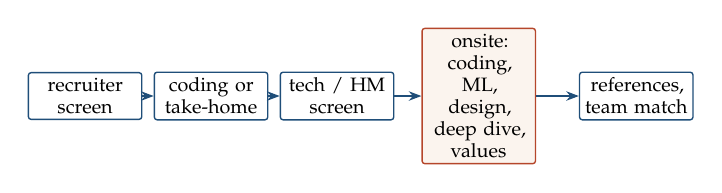
\begin{tikzpicture}[x=1mm,y=1mm,every node/.style={font=\tiny}]
\foreach \x/\t/\c in {0/{recruiter\\screen}/box,16/{coding or\\take-home}/box,32/{tech / HM\\screen}/box,50/{onsite: coding, ML,\\design, deep dive,\\values}/hbox,70/{references,\\team match}/box}{
  \node[\c,text width=13mm] (n\x) at (\x,0) {\t};}
\draw[arr] (n0)--(n16); \draw[arr] (n16)--(n32); \draw[arr] (n32)--(n50); \draw[arr] (n50)--(n70);
\end{tikzpicture}
\end{center}

\begin{mem}[What each lab emphasizes (reported, varies by team and year)]
\begin{tabularx}{\linewidth}{@{}lL@{}}
\toprule
Anthropic & practical multi-part coding (CodeSignal/Colab, can look things up), ML/system design, project deep dive, values round strong engineers underestimate; no AI in live rounds; perf take-home is public\\
OpenAI & practical coding that grows in scope, in your editor; ML depth and debugging for research roles; LLM system design; every project number probed\\
Google / GDM & DSA medium in 20--25 min, often without running code; GDM ``quiz'' (rapid math/stats/ML breadth); ML rounds; hiring committee; JAX helps\\
Meta & 2 DSA problems per 45 min; AI-enabled coding round in CoderPad (fix, implement, optimize); ML system design; behavioral by level (E4 vs E5 scope)\\
NVIDIA & C++/Python, CUDA execution model, memory hierarchy, roofline-style performance reasoning, DL fundamentals; outside AI tools disqualify\\\bottomrule
\end{tabularx}
\end{mem}

\begin{qa}[Round-by-round playbook]
\Q{Practical coding round: how to run it?}{Restate the spec, ask about scale and edge cases, write a tiny working version first, add tests as you go, narrate trade-offs, then extend. Clean names and small functions beat cleverness. Requirements will grow: design so step 2 is a small change.}
\Q{ML coding (``implement attention / BPE / DPO'')?}{State shapes before writing, write the core in 10 minutes, then test invariants (causality, equivalence to a library call, a gradient check). Mention dtype, masking and numerical stability unprompted (section~\ref{sec:code}).}
\Q{ML / LLM system design structure?}{Clarify goal and metric \ra\ constraints (QPS, latency, cost, privacy) \ra\ data \ra\ baseline \ra\ architecture diagram \ra\ evaluation offline/online \ra\ serving and scaling \ra\ failure modes, monitoring, iteration. Quantify with napkin math at each step.}
\Q{Project deep dive: what gets probed?}{Data (test set, size, split, leakage); numbers (metric with CI, baseline tuned equally?); choices (why this loss/model, what failed); costs (accuracy vs latency, on what hardware); next (10$\times$ compute, what would change your mind). Keep a numbers sheet per project.}
\Q{Research-taste questions?}{``Most surprising result you got'', ``a paper you think is wrong'', ``what would you work on with a cluster for a month''. Show a hypothesis, a cheap experiment to test it, and what result would falsify it.}
\Q{Values / mission round?}{Specific (named paper, policy, incident), personal (something you did), nuanced (state the strongest opposing view), calibrated (``I think X, I'd change my mind if Y''). Prepare one thing you'd refuse to build and one borderline case you'd accept with conditions.}
\end{qa}

\begin{center}
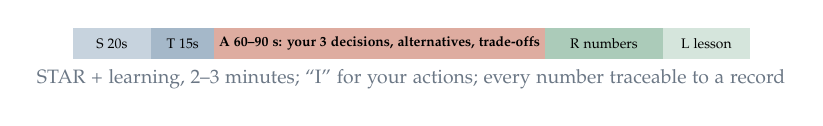
\begin{tikzpicture}[x=1mm,y=1mm,every node/.style={font=\tiny}]
\fill[acc!25] (0,0) rectangle (10,4); \node at (5,2) {S 20s};
\fill[acc!40] (10,0) rectangle (18,4); \node at (14,2) {T 15s};
\fill[acc2!45] (18,0) rectangle (60,4); \node at (39,2) {\textbf{A 60--90 s: your 3 decisions, alternatives, trade-offs}};
\fill[acc3!40] (60,0) rectangle (75,4); \node at (67.5,2) {R numbers};
\fill[acc3!20] (75,0) rectangle (86,4); \node at (80.5,2) {L lesson};
\node[lab] at (43,-2.5) {STAR + learning, 2--3 minutes; ``I'' for your actions; every number traceable to a record};
\end{tikzpicture}
\end{center}

\begin{mem}[Story bank: 12--15 true stories, each covering several themes]
\begin{tabularx}{\linewidth}{@{}lL@{}}
\toprule
hard technical problem & loss design, quantization trade-off, a bug you root-caused\\
ownership / ambiguity & a project you scoped from nothing\\
failure / mistake & badly scoped work and what you changed after\\
conflict / pushback & cost vs accuracy vs speed with a stakeholder\\
learning fast & a new domain in weeks; your from-scratch labs\\
leading without authority & contractors, cross-team asks\\
saying no & turning down bad-fit work\\
honesty under pressure & reporting a worse number than hoped\\
safety/privacy over speed & choosing on-prem/local for sensitive data\\
research taste & the most surprising experimental result\\\bottomrule
\end{tabularx}\par\smallskip
{\scriptsize Follow-up drill, three levels deep: How did you measure it? What else did you consider? What if you'd done nothing? Who disagreed? What would you change? Where did you apply the lesson since?}
\end{mem}

\begin{mem}[The 18 DSA patterns and their trigger signals]
\begin{tabularx}{\linewidth}{@{}lL@{}}
\toprule
two pointers & sorted array pair/triplet, merge two sequences, palindrome\\
sliding window & longest/shortest substring or subarray with a condition\\
binary search & sorted, find target/boundary, need $O(\log n)$\\
search on answer & ``smallest $X$ such that $Y$'', rotated array, peak\\
cyclic sort & values in $[1,N]$, find missing/duplicate\\
linked-list reversal & reverse (part of) list, reorder, cycle, middle\\
tree BFS & level by level, shortest path in tree, side views\\
tree DFS & path sums, construction, validation, LCA\\
graph BFS/DFS/topo & components, shortest unweighted path, cycles, dependency order\\
backtracking & all subsets/permutations, N-queens, Sudoku\\
greedy & interval scheduling, jump game, local choice provably optimal\\
two heaps & running median, split into two groups\\
top-$K$ & $k$-th largest, $k$ most frequent (size-$k$ heap)\\
$K$-way merge & merge $K$ sorted lists, $k$-th smallest in matrix\\
DP 1-D & number of ways, min/max cost, overlapping subproblems\\
DP 2-D & two strings (LCS, edit distance), grids\\
trie & prefix matching, word search, autocomplete\\
union-find & dynamic connectivity, counting components\\\bottomrule
\end{tabularx}\par\smallskip
{\scriptsize Standard: a medium in 20--25 min, narrated, with complexity and edge cases. Practise follow-ups: ``doesn't fit in memory'', ``now it's a stream'', ``now concurrent''.}
\end{mem}

\begin{trap}[Questions to ask them, and what not to ask]
HM: what success looks like at 6 months, the team's hardest open problem, how research becomes product. Engineers: how experiments are reviewed, eval culture, on-call. Skip-level: strategy for two years. Never ask what the website already answers.
\end{trap}

\section{``What would you do?'' debugging scenarios}
\lab{the round that separates people who have run things from people who have read about them}

\begin{center}
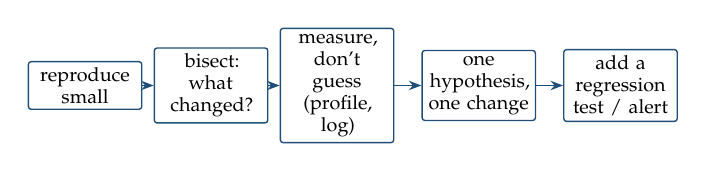
\begin{tikzpicture}[x=1mm,y=1mm,every node/.style={font=\tiny}]
\foreach \x/\t in {0/{reproduce\\small},16/{bisect: what\\changed?},32/{measure, don't\\guess (profile, log)},50/{one hypothesis,\\one change},68/{add a regression\\test / alert}}{
  \node[box,text width=13mm] (n\x) at (\x,0) {\t};}
\draw[arr] (n0)--(n16); \draw[arr] (n16)--(n32); \draw[arr] (n32)--(n50); \draw[arr] (n50)--(n68);
\end{tikzpicture}
\end{center}

\begin{qa}[Training]
\Q{Loss is NaN at step 3{,}000.}{Find the first non-finite tensor (anomaly mode or hooks on a replay of the batch). Usual causes: LR too high or no warmup, fp16 overflow (switch to bf16 or check the loss scaler), $\log(0)$ or division by zero in custom code, attention logits blowing up (QK-norm, z-loss), a corrupt batch. Rewind to the last good checkpoint, skip the batch, lower LR.}
\Q{Loss plateaus way above expected from step 0.}{Check initial loss $\approx\ln V$; overfit one batch (must go to $\approx0$); label shift by one; mask wrong; LR off by $10\times$; frozen params (\texttt{requires\_grad}); optimizer given the wrong param list; data shuffled into noise (tokenizer mismatch).}
\Q{GPU OOM after an innocent change.}{Longer sequences or bigger micro-batch (activations scale with $B\cdot T$), a tensor kept in a list for logging (holds the graph: use \texttt{.item()} or \texttt{.detach()}), eval without \texttt{no\_grad}, fragmentation (\texttt{expandable\_segments}). Fix with checkpointing, smaller micro-batch + accumulation, FSDP, fused CE for big vocabs.}
\Q{Throughput dropped 30\% after a library upgrade.}{Profile both versions on the same batch; compare kernel lists (a fused kernel replaced by an unfused path, FlashAttention fallback to math SDPA, recompilations in \texttt{torch.compile}), NCCL settings, data-loader workers. Pin versions in the image.}
\Q{Multi-node job hangs at startup or mid-run.}{A rank waiting at a collective others never reached (rank-dependent control flow, unequal batch counts, an exception on one rank). Set \texttt{NCCL\_DEBUG=INFO}, \texttt{TORCH\_NCCL\_ASYNC\_ERROR\_HANDLING}, timeouts; check \texttt{py-spy dump} on every rank; check the network fabric and a bad node.}
\Q{Validation loss improves but downstream evals get worse.}{Eval harness or prompt format changed; overfitting a narrow data mix; the eval was contaminated before and is now not; tokenizer/template mismatch at eval time; metric noise (check the CI).}
\end{qa}

\begin{qa}[Post-training and serving]
\Q{DPO: rewards margin rises, outputs get longer and worse.}{Both chosen and rejected log-probs falling (likelihood displacement); length exploitation in preferences. Lower LR, raise $\beta$, add SFT loss on chosen (RPO), length-normalize or length-control the data, check that pairs are on-policy.}
\Q{GRPO reward goes up, held-out accuracy flat.}{Reward hacking (format rewards, verifier holes), training on all-correct/all-wrong groups (zero advantage), entropy collapse (clip-higher, temperature), train/test prompt overlap. Read 20 samples before reading any curve.}
\Q{vLLM p99 latency spikes under load.}{KV cache full \ra\ preemption and recompute; long prompts blocking decode (enable chunked prefill); too large \texttt{max\_num\_seqs}; prefix cache misses after a prompt change. Check queue time vs prefill vs decode in metrics.}
\Q{Quantized model fine on benchmarks, worse for users.}{Benchmarks miss long-context, multilingual and tool-use regressions; outlier channels hurt by INT4; KV cache quantized too. Eval on production traffic samples, keep sensitive layers in higher precision, try AWQ/GPTQ with a domain calibration set.}
\Q{Outputs differ between batch sizes with greedy decoding.}{Non-determinism from batch-dependent kernels (reduction order in matmuls/attention), FP8/bf16 rounding; expected unless you use batch-invariant kernels. Compare log-prob differences, not strings.}
\Q{RAG answers are good offline, bad in production.}{Offline set not representative (query distribution shift), stale index, tenant filters dropping docs, chunking differs between pipelines, prompt truncation at the context limit. Log retrieved ids per request and replay.}
\Q{Agent loops forever calling the same tool.}{Tool errors not surfaced in a useful form, no step budget, ambiguous tool descriptions, missing ``done'' criterion. Return actionable error messages, cap steps, dedupe identical calls, add a final-answer tool.}
\end{qa}

\newpage
\section{Rapid fire: answer in one breath}
\lab{cover the right side, say the answer, check}

\begin{qa}[Fundamentals]
\RF{Why log-softmax not log(softmax)?}{numerical stability (LSE with max subtracted) + clean gradient $p-y$}
\RF{Why does label smoothing help?}{prevents over-confident logits; better calibration}
\RF{Dropout in LLM pretraining?}{usually 0: one epoch over huge data, little overfitting}
\RF{Weight tying?}{share embedding and LM head: saves $Vd$ params; common in small models}
\RF{Gradient clipping threshold?}{global norm 1.0; log the pre-clip norm}
\RF{Teacher forcing?}{train on ground-truth prefixes; inference sees its own outputs (exposure bias)}
\RF{Perplexity 20 in nats?}{$\ln20\approx3.0$}
\RF{Why GELU/SiLU over ReLU?}{smooth, non-zero gradient for negatives; empirically better}
\RF{Vanishing gradients in transformers prevented by?}{residuals + pre-norm + sane init}
\RF{Causal vs bidirectional attention mask?}{lower-triangular vs full}
\RF{What is a logit lens?}{decode intermediate residual streams with the final norm + unembedding}
\RF{Gradient checkpointing cost?}{$\approx$+33\% compute (one extra forward)}
\RF{Cross-entropy at uniform init?}{$\ln V$}
\RF{Embedding lookup FLOPs?}{none (a gather); its backward is scatter-add}
\end{qa}

\begin{qa}[Architecture]
\RF{Params of a GPT block ($4d$ GELU MLP, MHA)?}{$12d^2$}
\RF{GPT-2 small?}{124M: $d$768, $L$12, $H$12, $V$50{,}257, ctx 1024}
\RF{Llama-3-8B?}{$d$4096, $L$32, $H$32/$H_{kv}$8, $f$14336, $V$128k, RoPE $5{\cdot}10^5$}
\RF{Llama-3-70B KV/token?}{320 KiB (80 layers, 8 KV heads)}
\RF{Why RoPE over learned absolute?}{relative by construction, no params, works with KV cache, extendable}
\RF{ALiBi?}{linear distance bias per head; extrapolates, recency-biased}
\RF{Mixtral?}{8 experts, top-2, 46.7B total / 12.9B active}
\RF{DeepSeek-V3?}{671B / 37B active, MLA, 256+1 experts top-8, MTP, FP8 training}
\RF{Why no biases in LLMs?}{fewer drifting params, simpler sharding/quant, no quality loss}
\RF{Sliding window $W$ over $L$ layers reaches?}{$L\cdot W$ tokens (not reliably)}
\RF{Mamba vs attention, recall?}{fixed state $\approx$ KV of 64 tokens; weak exact recall}
\RF{QK-norm fixes?}{attention-logit growth}
\RF{Multi-token prediction?}{extra heads/modules predict $t{+}2..$; denser signal; drafts for spec decoding}
\RF{Parallel attention + MLP block (GPT-J, PaLM)?}{$x+\mathrm{Attn}(n(x))+\mathrm{MLP}(n(x))$: one fused matmul, $\sim$15\% faster}
\end{qa}

\begin{qa}[Training and scaling]
\RF{Chinchilla-optimal tokens for 7B?}{$\approx$140B (20/param)}
\RF{Training FLOPs, 7B on 2T tokens?}{$6\cdot7\!\cdot\!10^9\cdot2\!\cdot\!10^{12}\approx8.4\!\cdot\!10^{22}$}
\RF{Days on 256 H100 at 40\% MFU?}{$8.4\!\cdot\!10^{22}/(256\cdot989\!\cdot\!10^{12}\cdot0.4)\approx9.6$ days}
\RF{Memory for AdamW on 70B?}{$16\times70$B $=$ 1.12 TB before activations}
\RF{ZeRO stage that shards weights?}{3 (FSDP full-shard)}
\RF{Pipeline bubble formula?}{$(p-1)/(m+p-1)$}
\RF{Where does TP live?}{inside a node, over NVLink}
\RF{MoE comm primitive?}{all-to-all}
\RF{Why ramp batch size?}{critical batch grows as loss falls}
\RF{Loss spike remedy?}{rewind $\sim$100 steps, skip batches, lower LR; QK-norm, z-loss}
\RF{$\beta_2$ for LLMs?}{0.95}
\RF{Weight decay applied to norms?}{no (nor biases, often embeddings)}
\RF{Peak LR for 7B AdamW?}{$\sim$3e-4 (confirm on a proxy / $\mu$P)}
\RF{Repeated-data limit?}{$\sim$4 epochs nearly as good as fresh}
\RF{FineWeb MinHash setup?}{5-grams, 112 hashes $=$ 14 bands $\times$ 8 rows, $\sim$0.75 Jaccard}
\end{qa}

\begin{qa}[Post-training]
\RF{SFT loss on prompt tokens?}{no; mask with $-100$; include end-of-turn}
\RF{LoRA trainable params per matrix?}{$r(d_\text{in}+d_\text{out})$}
\RF{LoRA LR vs full FT?}{$\sim$10$\times$ higher}
\RF{QLoRA bits per param?}{$\approx$4.5 (NF4 + fp32 scale per 64) $\to$ $\sim$4.13 w/ double quant}
\RF{DPO $\beta$ default?}{0.1 (range 0.01--0.5); smaller lets policy move further}
\RF{DPO implicit reward?}{$\beta\log\pi_\theta(y|x)/\pi_\text{ref}(y|x)$}
\RF{Why does $Z(x)$ vanish in DPO?}{it depends only on $x$; cancels in $r_w-r_l$}
\RF{PPO clip $\varepsilon$?}{0.2}
\RF{PPO models in memory?}{4: policy, value, ref, reward}
\RF{GRPO group size?}{$G\approx8$--64; advantage $(r-\bar r)/\sigma$}
\RF{DAPO clip-higher?}{$\varepsilon_\text{low}{=}0.2,\varepsilon_\text{high}{=}0.28$}
\RF{Dr.\,GRPO removes?}{per-sequence length norm and std normalization}
\RF{KL estimator in GRPO?}{$k_3=\rho-1-\log\rho$}
\RF{Reasoning RL on all-correct groups?}{zero advantage: drop them (dynamic sampling)}
\RF{RLHF KL direction?}{reverse, $\KL(\pi\|\pi_\text{ref})$}
\RF{On-policy distillation reward?}{per-token $-(\log q_\theta-\log p_\text{teacher})$}
\end{qa}

\begin{qa}[Inference]
\RF{Batch-1 decode bound?}{BW / weight bytes (8B bf16 on H100 $\approx$ 200 tok/s)}
\RF{Prefill intensity?}{$\approx P$ (prompt length) $\Rightarrow$ compute-bound}
\RF{Decode intensity?}{$\approx B$ for weights, $\approx1$ (or $g$ with GQA) for KV}
\RF{vLLM block size?}{16 tokens}
\RF{KV waste before/after paging?}{60--80\% \ra\ $<$4\%}
\RF{Spec decode tokens per round?}{$(1-\alpha^{k+1})/(1-\alpha)$}
\RF{Spec decode acceptance rule?}{accept w.p.\ $\min(1,p/q)$; else sample $\mathrm{norm}(\max(0,p-q))$}
\RF{FP8 for inference?}{e4m3 (max 448)}
\RF{GPTQ uses?}{inverse Hessian $H=2X^\top X$ to push rounding error to later columns}
\RF{AWQ protects?}{$\sim$1\% salient channels by activation scale}
\RF{SmoothQuant $\alpha$?}{$\approx0.5$; migrates difficulty from activations to weights}
\RF{INT4 g128 bits/weight?}{4.125}
\RF{Online softmax state?}{running max $m$, running sum $\ell$, accumulator $o$}
\RF{TTFT is dominated by?}{queueing + prefill}
\RF{Prefix cache killer?}{dynamic content (timestamps) early in the prompt}
\RF{Chunked prefill benefit?}{no decode stalls; uses idle FLOPs}
\RF{Min-$p$ sampling?}{keep tokens with $p\ge p_\text{min}\cdot p_\text{max}$}
\end{qa}

\begin{qa}[Eval, RAG, agents, safety]
\RF{95\% CI, 1{,}000 items at 70\%?}{$\pm$2.8 points}
\RF{Halve the CI?}{4$\times$ the items}
\RF{pass@$k$ estimator?}{$1-\binom{n-c}{k}/\binom nk$}
\RF{$\kappa$ with $p_o{=}.85$, $p_e{=}.68$?}{0.53}
\RF{RRF constant?}{$k=60$}
\RF{Most important retrieval metric for RAG?}{recall@$k$}
\RF{Contextual retrieval gain?}{$-$49\% failures; $-$67\% with reranking}
\RF{Lost in the middle?}{mid-context info used worst; put key passages at ends}
\RF{IVF nlist rule of thumb?}{$\sim\!\sqrt N$ (4--16$\sqrt N$)}
\RF{Agent 0.99/step, 50 steps?}{61\%}
\RF{pass$^8$ at 90\%?}{43\%}
\RF{Lethal trifecta?}{private data + untrusted content + exfil channel}
\RF{Refusal in open models mediated by?}{one direction in the residual stream}
\RF{Induction head pattern?}{\dots A B \dots A $\to$ B, via K-composition}
\RF{SAE metrics?}{L0, FVU, $\Delta$CE, dead latents, auto-interp}
\RF{FID measures?}{distance between Inception-feature Gaussians, real vs generated}
\RF{CFG formula?}{$\epsilon_\varnothing+w(\epsilon_c-\epsilon_\varnothing)$}
\end{qa}

\needspace{16\baselineskip}
\begin{mem}[Napkin constants]
\begin{tabularx}{\linewidth}{@{}lL@{}}
\toprule
1 token & $\approx$ 4 English characters $\approx$ 0.75 words\\
H100 SXM & 989 TF/s bf16, 1{,}979 FP8 dense, 3.35 TB/s, 80 GB, NVLink 900 GB/s\\
H100 ridge & $\approx$295 FLOP/byte (bf16)\\
A100 80G & 312 TF/s, 2.0 TB/s\\
PCIe 5 x16 & 64 GB/s per direction\\
IB NDR & 400 Gb/s $=$ 50 GB/s\\
bytes/param & fp32 4, bf16 2, fp8 1, int4 0.5\\
train state & 16 B/param (AdamW mixed precision)\\
KV (GQA-8, 128 dh) & $2\cdot L\cdot8\cdot128\cdot2=4L$ KiB/token\\
GPT-2 init loss & 10.82 \quad Llama 3: 11.76 \quad Llama 2: 10.37\\
$\sqrt{128}$ & 11.3 \quad $1/\sqrt{4096}=1/64$\\
$e^{-1}$, $\ln2$ & 0.368, 0.693\\\bottomrule
\end{tabularx}
\end{mem}

\section{Formula sheet: write each from memory}
\lab{cover the page, rewrite, compare}

{\small
\newcommand{\F}[2]{\par\noindent{\sffamily\bfseries\scriptsize\color{acc}#1}\par\nopagebreak\vspace{-1pt}\noindent\hspace*{0.6em}#2\par\vspace{2.5pt}}

\paragraph{Core layers}
\F{Scaled dot-product attention}{$\mathrm{Attn}(Q,K,V)=\softmax\!\big(QK^\top/\sqrt{d_h}+M\big)V$, $M_{ij}=-\infty$ for $j>i$}
\F{Multi-head}{$\mathrm{MHA}(x)=[\,h_1;\dots;h_H\,]W_O$, $h_i=\mathrm{Attn}(xW_Q^i,xW_K^{g(i)},xW_V^{g(i)})$, $g$ maps heads to KV groups}
\F{RMSNorm / LayerNorm}{$\frac{x}{\sqrt{\frac1d\sum x_i^2+\epsilon}}\odot g$ \quad / \quad $\frac{x-\mu}{\sqrt{\sigma^2+\epsilon}}\odot g+b$}
\F{SwiGLU MLP}{$\big(\mathrm{SiLU}(xW_g)\odot xW_u\big)W_d$, $\mathrm{SiLU}(z)=z\,\sigma(z)$}
\F{RoPE (pair $i$, position $m$)}{$\theta_i=b^{-2i/d_h}$; $(x_{2i},x_{2i+1})\mapsto R(m\theta_i)(x_{2i},x_{2i+1})$; $\langle R_mq,R_nk\rangle=f(q,k,m-n)$}
\F{Pre-norm block}{$h=x+\mathrm{Attn}(\mathrm{N}(x))$;\quad $y=h+\mathrm{MLP}(\mathrm{N}(h))$}
\F{Softmax-CE gradient}{$\partial L/\partial z=\softmax(z)-e_y$}

\paragraph{Optimization}
\F{AdamW}{$m\leftarrow\beta_1m+(1-\beta_1)g$, $v\leftarrow\beta_2v+(1-\beta_2)g^2$, $\theta\leftarrow\theta-\eta\big(\frac{\hat m}{\sqrt{\hat v}+\epsilon}+\lambda\theta\big)$, $\hat m=\frac{m}{1-\beta_1^t}$}
\F{Cosine schedule}{$\eta_t=\eta_\text{min}+\frac12(\eta_\text{max}-\eta_\text{min})(1+\cos(\pi t/T))$ after linear warmup}
\F{Kaiming / Xavier}{$\mathrm{Var}(W)=2/n_\text{in}$ (ReLU) \quad / \quad $2/(n_\text{in}+n_\text{out})$}
\F{Grad clipping}{$g\leftarrow g\cdot\min(1,c/\|g\|_2)$}

\paragraph{Scaling and compute}
\F{FLOPs}{forward $\approx2N$ per token; training $C\approx6ND$; attention adds $\approx 4\,L\,T\,d$ per token forward (causal halves it)}
\F{Chinchilla loss}{$L(N,D)=E+A/N^\alpha+B/D^\beta$, $\alpha\approx\beta\approx0.3$ \ra\ $N^*\propto C^{0.5}$, $D^*\approx20N^*$}
\F{Memory}{train $\approx16N$ bytes (bf16 W,G + fp32 master, $m$, $v$); KV $=2\cdot L\cdot H_{kv}\cdot d_h\cdot b$ bytes/token}
\F{Roofline}{$\text{attainable}=\min(\text{peak},\ I\cdot\text{BW})$, $I=$ FLOPs/byte; ridge $=$ peak/BW}
\F{Pipeline bubble}{$(p-1)/(m+p-1)$;\quad ring all-reduce bytes/GPU $=2\frac{n-1}{n}S$}

\paragraph{Post-training}
\F{RLHF objective and optimum}{$\max_\pi\E[r]-\beta\KL(\pi\|\pi_\text{ref})$ \ra\ $\pi^*\propto\pi_\text{ref}\,e^{r/\beta}$}
\F{Bradley--Terry RM loss}{$-\log\sigma(r(x,y_w)-r(x,y_l))$}
\F{DPO}{$-\log\sigma\!\Big(\beta\big[\log\frac{\pi_\theta(y_w|x)}{\pi_\text{ref}(y_w|x)}-\log\frac{\pi_\theta(y_l|x)}{\pi_\text{ref}(y_l|x)}\big]\Big)$}
\F{PPO clip}{$\E\big[\min(\rho A,\ \mathrm{clip}(\rho,1{-}\epsilon,1{+}\epsilon)A)\big]$, $\rho=\pi_\theta/\pi_\text{old}$}
\F{GAE}{$\delta_t=r_t+\gamma V_{t+1}-V_t$, $A_t=\sum_l(\gamma\lambda)^l\delta_{t+l}$}
\F{GRPO advantage, KL}{$A_i=(r_i-\bar r)/\sigma_r$ over $G$ samples; $k_3=\rho-1-\log\rho$ with $\rho=\pi_\text{ref}/\pi_\theta$}
\F{Policy gradient}{$\nabla J=\E\big[\nabla\log\pi_\theta(y|x)\,(R-b)\big]$}
\F{LoRA}{$W=W_0+\frac{\alpha}{r}BA$, $B\in\mathbb R^{d\times r}=0$ at init}

\paragraph{Inference}
\F{Sampling}{$p_i\propto e^{z_i/T}$; top-$p$: smallest set with $\sum p\ge p$; min-$p$: $p_i\ge p_\text{min}\,p_\text{max}$}
\F{Speculative decoding}{accept w.p.\ $\min(1,p/q)$; else sample $\propto\max(0,p-q)$; $\E[\text{tokens}]=\frac{1-\alpha^{k+1}}{1-\alpha}$}
\F{Online softmax}{$m'=\max(m,\max s)$, $\ell'=\ell e^{m-m'}+\sum e^{s-m'}$, $o'=oe^{m-m'}+e^{s-m'}V$}
\F{Quantization}{$q=\mathrm{clip}(\mathrm{round}(x/s)+z)$, $s=(\max-\min)/(2^b-1)$ (asym) or $\max|x|/(2^{b-1}-1)$ (sym)}

\paragraph{Evaluation and retrieval}
\F{Binomial CI}{$\hat p\pm1.96\sqrt{\hat p(1-\hat p)/n}$;\quad sample size for effect $\delta$: $n\approx(z_{\alpha/2}+z_\beta)^2\,2p(1-p)/\delta^2$}
\F{pass@$k$ (unbiased)}{$1-\binom{n-c}{k}\big/\binom{n}{k}$}
\F{Cohen's $\kappa$}{$(p_o-p_e)/(1-p_e)$}
\F{InfoNCE}{$-\log\frac{e^{s(q,d^+)/\tau}}{\sum_j e^{s(q,d_j)/\tau}}$}
\F{BM25}{$\sum_t\mathrm{idf}(t)\frac{f(t,d)(k_1+1)}{f(t,d)+k_1(1-b+b\,|d|/\overline{|d|})}$, $k_1\approx1.2$, $b\approx0.75$}
\F{RRF, nDCG}{$\sum_r\frac1{60+\mathrm{rank}_r(d)}$;\quad $\mathrm{DCG}=\sum_i\frac{2^{rel_i}-1}{\log_2(i+1)}$}

\paragraph{Generative models}
\F{DDPM}{$x_t=\sqrt{\bar\alpha_t}x_0+\sqrt{1-\bar\alpha_t}\,\epsilon$; loss $\|\epsilon-\epsilon_\theta(x_t,t)\|^2$}
\F{Classifier-free guidance}{$\hat\epsilon=\epsilon_\varnothing+w(\epsilon_c-\epsilon_\varnothing)$}
\F{Flow matching}{$x_t=(1-t)x_0+t\,\epsilon$, regress $v_\theta(x_t,t)\approx\epsilon-x_0$}
\F{VAE ELBO}{$\log p(x)\ge\E_q[\log p(x|z)]-\KL(q(z|x)\|p(z))$}
}

\section{Paper cards: what to say in 20 seconds}
\lab{curriculum/papers.md \textperiodcentered\ claim, key number, limitation}

{\small
\newcommand{\PC}[3]{\par\noindent\hangindent=0.9em\hangafter=1{\sffamily\bfseries\color{acc}#1}\ \ #2\ {\color{acc2}\textit{Limit:} #3}\par\vspace{1pt}}
\PC{Attention Is All You Need (2017)}{Encoder--decoder of attention + MLP, no recurrence; parallel training; 28.4 BLEU EN--DE.}{quadratic in length; sinusoidal positions extrapolate poorly.}
\PC{GPT-2 (2019)}{1.5B decoder LM trained on WebText does tasks zero-shot; pre-norm.}{zero-shot far below fine-tuned SOTA.}
\PC{GPT-3 (2020)}{175B, few-shot in-context learning improves smoothly with scale.}{weak on reasoning; prompt sensitivity; not compute-optimal.}
\PC{Kaplan scaling laws (2020)}{Loss is a power law in $N$, $D$, $C$; bigger models are more sample-efficient.}{fixed LR schedule biased the $N$ vs $D$ split.}
\PC{Chinchilla (2022)}{IsoFLOP sweeps: scale $N$ and $D$ equally; 70B/1.4T beats 280B Gopher.}{ignores inference cost; real models over-train.}
\PC{InstructGPT (2022)}{SFT + RM + PPO; 1.3B preferred to 175B GPT-3 by raters.}{alignment tax; reward hacking; rater bias.}
\PC{LoRA (2021) / QLoRA (2023)}{Low-rank adapters match full FT on many tasks with $\sim$0.1--1\% params; QLoRA fine-tunes 65B on one 48 GB GPU via NF4.}{learns less and forgets less than full FT; weaker for new knowledge.}
\PC{FlashAttention (2022)}{IO-aware tiling + online softmax: exact attention, $O(T)$ memory, 2--4$\times$ faster.}{kernel engineering per hardware generation.}
\PC{PagedAttention / vLLM (2023)}{KV in fixed blocks with block tables: near-zero fragmentation, 2--4$\times$ throughput.}{indirection overhead in kernels.}
\PC{Speculative decoding (2023)}{Draft + verify with rejection sampling: identical distribution, 2--3$\times$ speedups.}{gains shrink at large batch (compute-bound).}
\PC{DPO (2023)}{Closed-form RLHF optimum turns preference learning into a classification loss; no RM, no sampling.}{offline; likelihood displacement; sensitive to data distribution.}
\PC{LLaMA (2023)}{Open 7--65B models trained past Chinchilla on public data; 13B rivals GPT-3.}{data and license constraints.}
\PC{Mixtral (2023)}{8 experts top-2: 47B total / 13B active matches Llama-2-70B.}{memory of all experts at serve time.}
\PC{GPTQ (2022) / AWQ (2023)}{3--4-bit weight-only quantization with small loss via Hessian compensation / salient-channel scaling.}{activation outliers still hard; calibration-set dependence.}
\PC{Toy Models of Superposition (2022)}{Sparse features get packed into fewer dimensions; explains polysemanticity.}{toy setting.}
\PC{In-context learning and induction heads (2022)}{Induction heads form in a phase change that coincides with ICL gains.}{causal evidence strongest in small models.}
\PC{Lost in the Middle (2023)}{Models use information at the start/end of context best; U-shaped accuracy.}{newer long-context training reduces it.}
\PC{RAG (2020)}{Retriever + generator trained jointly; better factuality on open QA.}{retrieval errors propagate.}
\PC{DeepSeekMath / GRPO (2024)}{Group-relative advantages remove the value network; strong math RL.}{length bias, std normalization issues (Dr.\,GRPO).}
\PC{DeepSeek-V3 (2024)}{671B/37B MoE, MLA, aux-loss-free balancing, MTP, FP8 training for $\sim$2.8M H800-hours.}{complex to serve; reported cost excludes research.}
\PC{DeepSeek-R1 (2025)}{RL on verifiable rewards yields long CoT reasoning; distilled small models are strong.}{readability, language mixing (R1-Zero); verifiable domains only.}
\PC{Sparse autoencoders at scale (2024)}{Monosemantic, steerable features in production-size models.}{dead latents, absorption, reconstruction error.}
\PC{Scaling test-time compute (2024)}{Compute-optimal mix of sampling and revision can beat a 14$\times$ larger model on some problems.}{needs good verifiers; problem-difficulty dependent.}
}

\section{Glossary A--Z}
{\small
\newcommand{\G}[2]{\par\noindent\hangindent=0.9em\hangafter=1{\sffamily\bfseries\color{acc}#1}\ \ #2\par}
\G{ABF}{adjusted base frequency: raise RoPE base before long-context training.}
\G{Activation checkpointing}{store few activations, recompute in backward; +33\% compute.}
\G{AdamW}{Adam with decoupled weight decay.}
\G{Alignment tax}{capability lost to safety/preference tuning.}
\G{All-reduce / all-gather / reduce-scatter / all-to-all}{the four collectives (section~\ref{sec:compute}).}
\G{Attention sink}{first tokens absorb attention mass; keep them when evicting KV (StreamingLLM).}
\G{AWQ / GPTQ}{4-bit weight quantization: salient-channel scaling / Hessian error compensation.}
\G{Beam search}{keep top-$b$ partial sequences by log-prob; bland for chat.}
\G{BPE}{byte-pair encoding: merge most frequent pairs.}
\G{Bradley--Terry}{$P(a\succ b)=\sigma(r_a-r_b)$; RMs, DPO, arenas.}
\G{Capacity factor}{expert buffer size multiplier in MoE; overflow tokens dropped.}
\G{Chat template}{serialization of roles with special tokens; must match training.}
\G{Chinchilla}{70B on 1.4T tokens; compute-optimal $\approx$20 tokens/param.}
\G{Chunked prefill}{split prompts into budgeted chunks interleaved with decode.}
\G{Constitutional AI}{self-critique against written principles + RLAIF.}
\G{Context parallelism}{shard the sequence across GPUs for attention (ring).}
\G{Continuous batching}{batch re-formed every decode step.}
\G{Contrastive loss}{InfoNCE: pull positives together, push negatives apart.}
\G{Cross-encoder}{scores query and doc jointly; reranking.}
\G{DPO / IPO / KTO / SimPO / ORPO}{preference objectives without RL (section~\ref{sec:post}).}
\G{Distillation}{train a student on a teacher's outputs or logits.}
\G{Double descent}{test error falls again past the interpolation threshold.}
\G{Emergence}{abrupt task gains; often an artifact of discontinuous metrics.}
\G{Expert parallelism}{experts on different GPUs; all-to-all dispatch.}
\G{Exposure bias}{train on gold prefixes, generate on own prefixes.}
\G{FlashAttention}{IO-aware tiled exact attention with online softmax.}
\G{FSDP / ZeRO}{shard params, grads, optimizer states across data-parallel ranks.}
\G{Function calling}{model emits structured tool calls validated against JSON Schema.}
\G{GAE}{generalized advantage estimation, $\lambda$-weighted TD errors.}
\G{GQA / MQA / MLA}{fewer KV heads / one KV head / latent-compressed KV.}
\G{Grokking}{sudden generalization long after memorizing training data.}
\G{GRPO}{group-relative PPO without a value net (section~\ref{sec:post}).}
\G{Hallucination}{fluent unsupported content; measure faithfulness.}
\G{HNSW / IVF-PQ}{graph-based / clustered + compressed ANN indexes.}
\G{In-context learning}{learning from examples in the prompt, no weight update.}
\G{Induction head}{copy circuit \dots A B \dots A $\to$ B.}
\G{Instruction hierarchy}{train to prioritize system $>$ user $>$ tool text.}
\G{KV cache}{stored keys/values of past tokens; $2LH_{kv}d_h$ elems/token.}
\G{Label smoothing}{target $(1-\epsilon)$ on gold, $\epsilon$ spread elsewhere.}
\G{LoRA / QLoRA / DoRA}{low-rank adapters / on 4-bit base / magnitude--direction split.}
\G{Lost in the middle}{models use mid-context information worst.}
\G{Matryoshka embedding}{prefixes of the vector are valid embeddings.}
\G{MCP}{Model Context Protocol: standard tool/resource servers.}
\G{MFU / HFU}{useful FLOPs / all FLOPs incl.\ recompute, over peak.}
\G{Mixture of experts}{router picks top-$k$ expert MLPs per token.}
\G{Model collapse}{degradation from recursive training on own synthetic data.}
\G{$\mu$P}{parameterization making hyperparameters width-transferable.}
\G{Muon}{orthogonalized momentum for matrix params.}
\G{NF4}{4-bit NormalFloat levels at normal quantiles.}
\G{Online softmax}{streaming softmax with running max and sum.}
\G{PagedAttention}{KV in fixed blocks via block tables.}
\G{pass@$k$ / pass$^k$}{any of $k$ succeeds / all $k$ succeed.}
\G{Perplexity}{$\exp$ of mean NLL per token.}
\G{PPO}{clipped surrogate policy optimization.}
\G{Prefix caching}{reuse KV of shared prompt prefixes.}
\G{Prompt injection}{untrusted text hijacks model instructions.}
\G{PRM / ORM}{process vs outcome reward models.}
\G{QK-norm}{normalize $q,k$ to stop logit growth.}
\G{RAG}{retrieve then generate with citations.}
\G{Reward hacking}{exploiting reward flaws instead of solving the task.}
\G{RLHF / RLAIF / RLVR}{RL from human / AI feedback / verifiable rewards.}
\G{RMSNorm}{scale by root-mean-square, no centering.}
\G{RoPE / YaRN / NTK}{rotary positions and their extension tricks.}
\G{RRF}{reciprocal rank fusion, $\sum1/(60+\text{rank})$.}
\G{SAE}{sparse autoencoder dictionary over activations.}
\G{Self-consistency}{majority vote over sampled CoTs.}
\G{Speculative decoding}{draft $k$ tokens, verify in one target pass, exact.}
\G{Superposition}{more features than dimensions, almost-orthogonal.}
\G{SwiGLU}{gated MLP with SiLU; hidden $\approx8d/3$.}
\G{Sycophancy}{agreeing with the user over the truth.}
\G{Tensor parallelism}{split each matmul across GPUs (Megatron).}
\G{Test-time compute}{spend inference FLOPs (CoT, sampling, search) for accuracy.}
\G{Tied embeddings}{embedding matrix reused as LM head.}
\G{Top-$k$ / top-$p$ / min-$p$}{truncation sampling rules.}
\G{WSD}{warmup--stable--decay LR schedule.}
\G{z-loss}{penalty on $\log^2 Z$ to keep logits bounded.}
}

\section{References: the canon, by section}
{\small\raggedright
\newcommand{\rf}[2]{\par\noindent\hangindent=1em\hangafter=1 #1 {\color{mute}\ttfamily\scriptsize #2}\par}

\paragraph{Math, optimization (1, 3)}
\rf{Parr \& Howard, \emph{The Matrix Calculus You Need for Deep Learning}.}{explained.ai}
\rf{Kingma \& Ba 2014, \emph{Adam}.}{1412.6980}
\rf{Loshchilov \& Hutter 2019, \emph{Decoupled Weight Decay} (AdamW).}{1711.05101}
\rf{McCandlish et al.\ 2018, \emph{Empirical Model of Large-Batch Training}.}{1812.06162}
\rf{Yang et al.\ 2022, \emph{Tensor Programs V} ($\mu$P).}{2203.03466}
\rf{Wortsman et al.\ 2023, \emph{Small-scale proxies for large-scale instabilities}.}{2309.14322}
\rf{H\"agele et al.\ 2024, \emph{Scaling laws beyond fixed durations} (WSD).}{2405.18392}

\paragraph{Hardware (2)}
\rf{He, \emph{Making Deep Learning Go Brrrr}; DeepMind, \emph{How to Scale Your Model}; HF \emph{Ultra-Scale Playbook}.}{blogs}
\rf{Korthikanti et al.\ 2022, \emph{Reducing Activation Recomputation}.}{2205.05198}

\paragraph{Transformers, tokenizers (4, 5)}
\rf{Vaswani et al.\ 2017, \emph{Attention Is All You Need}.}{1706.03762}
\rf{Sennrich et al.\ 2016, \emph{BPE for NMT}; Kudo 2018, \emph{SentencePiece}.}{1508.07909, 1808.06226}
\rf{Su et al.\ 2021, \emph{RoFormer} (RoPE).}{2104.09864}
\rf{Shazeer 2019, MQA; Ainslie et al.\ 2023, GQA.}{1911.02150, 2305.13245}
\rf{Shazeer 2020, \emph{GLU Variants}; Zhang \& Sennrich 2019, RMSNorm.}{2002.05202, 1910.07467}
\rf{Xiong et al.\ 2020, \emph{On LayerNorm in the Transformer} (pre-LN).}{2002.04745}
\rf{Chen et al.\ 2023, PI; Peng et al.\ 2023, YaRN.}{2306.15595, 2309.00071}
\rf{Fedus et al.\ 2021, \emph{Switch Transformers}.}{2101.03961}
\rf{DeepSeek-V2 (MLA) and DeepSeek-V3 reports.}{2405.04434, 2412.19437}
\rf{Llama Team 2024, \emph{The Llama 3 Herd of Models}.}{2407.21783}
\rf{Gu \& Dao 2023, \emph{Mamba}.}{2312.00752}

\paragraph{Pretraining (6)}
\rf{Kaplan et al.\ 2020; Hoffmann et al.\ 2022 (Chinchilla); Besiroglu et al.\ 2024 (replication).}{2001.08361, 2203.15556, 2404.10102}
\rf{Sardana et al.\ 2023, \emph{Beyond Chinchilla-Optimal}.}{2401.00448}
\rf{Penedo et al.\ 2024, \emph{FineWeb}; Li et al.\ 2024, \emph{DCLM}.}{2406.17557, 2406.11794}
\rf{Lee et al.\ 2021, \emph{Deduplicating Training Data}; Muennighoff et al.\ 2023, \emph{Data-Constrained Scaling}.}{2107.06499, 2305.16264}
\rf{Rajbhandari et al.\ 2020, \emph{ZeRO}; Zhao et al.\ 2023, \emph{FSDP}.}{1910.02054, 2304.11277}
\rf{Shoeybi et al.\ 2019, Megatron-LM; Narayanan et al.\ 2021, PTD-P.}{1909.08053, 2104.04473}
\rf{Liu et al.\ 2023, \emph{Ring Attention}.}{2310.01889}

\paragraph{Post-training (7)}
\rf{Ouyang et al.\ 2022, InstructGPT; Christiano et al.\ 2017, RLHF.}{2203.02155, 1706.03741}
\rf{Schulman et al.\ 2017, PPO; 2015, GAE.}{1707.06347, 1506.02438}
\rf{Rafailov et al.\ 2023, DPO; Azar et al.\ IPO; Ethayarajh et al.\ KTO; Meng et al.\ SimPO.}{2305.18290, 2310.12036, 2402.01306, 2405.14734}
\rf{Shao et al.\ 2024, DeepSeekMath (GRPO); DeepSeek-R1 2025.}{2402.03300, 2501.12948}
\rf{Yu et al.\ 2025, DAPO; Liu et al.\ 2025, Dr.\,GRPO; Zheng et al.\ 2025, GSPO.}{2503.14476, 2503.20783, 2507.18071}
\rf{Hu et al.\ 2021, LoRA; Dettmers et al.\ 2023, QLoRA.}{2106.09685, 2305.14314}
\rf{Gao et al.\ 2022, \emph{RM Overoptimization}; Bai et al.\ 2022, \emph{Constitutional AI}.}{2210.10760, 2212.08073}
\rf{Lightman et al.\ 2023, \emph{Let's Verify Step by Step}; Snell et al.\ 2024, test-time compute.}{2305.20050, 2408.03314}
\rf{Wei et al.\ 2022, CoT; Wang et al.\ 2022, self-consistency.}{2201.11903, 2203.11171}
\rf{Hinton et al.\ 2015, distillation; Agarwal et al.\ 2024, on-policy distillation (GKD).}{1503.02531, 2306.13649}

\paragraph{Inference (8)}
\rf{Pope et al.\ 2022, \emph{Efficiently Scaling Transformer Inference}.}{2211.05102}
\rf{Dao et al.\ 2022 FlashAttention; Dao 2023 FA-2; Shah et al.\ 2024 FA-3.}{2205.14135, 2307.08691, 2407.08608}
\rf{Kwon et al.\ 2023, PagedAttention (vLLM); Zheng et al.\ 2024, SGLang.}{2309.06180, 2312.07104}
\rf{Agrawal et al.\ 2024, Sarathi-Serve; Zhong et al.\ 2024, DistServe.}{2403.02310, 2401.09670}
\rf{Leviathan et al.\ 2023; Chen et al.\ 2023, speculative sampling; Medusa; EAGLE.}{2211.17192, 2302.01318, 2401.10774, 2401.15077}
\rf{Frantar et al.\ GPTQ; Lin et al.\ AWQ; Xiao et al.\ SmoothQuant; Dettmers et al.\ LLM.int8().}{2210.17323, 2306.00978, 2211.10438, 2208.07339}

\paragraph{Evaluation (9)}
\rf{Miller 2024, \emph{Adding Error Bars to Evals}.}{2411.00640}
\rf{Chen et al.\ 2021, Codex / pass@$k$; Zheng et al.\ 2023, LLM-as-a-Judge.}{2107.03374, 2306.05685}
\rf{Biderman et al.\ 2024, \emph{Reproducible Evaluation}; Oren et al.\ 2023, contamination.}{2405.14782, 2310.17623}
\rf{Yao et al.\ 2024, $\tau$-bench; Jimenez et al.\ SWE-bench; Kwa et al.\ 2025, METR horizons.}{2406.12045, 2310.06770, 2503.14499}

\paragraph{Interpretability and safety (10)}
\rf{Elhage et al.\ 2021, \emph{Mathematical Framework for Transformer Circuits}.}{transformer-circuits.pub}
\rf{Olsson et al.\ 2022, \emph{Induction Heads}; Elhage et al.\ 2022, \emph{Toy Models of Superposition}.}{2209.11895, 2209.10652}
\rf{Bricken et al.\ 2023, \emph{Towards Monosemanticity}; Gao et al.\ 2024, TopK SAEs.}{t-c.pub, 2406.04093}
\rf{Wang et al.\ 2022, IOI circuit; Arditi et al.\ 2024, refusal direction.}{2211.00593, 2406.11717}
\rf{Greshake et al.\ 2023, indirect prompt injection; Hubinger et al.\ 2024, Sleeper Agents.}{2302.12173, 2401.05566}
\rf{Greenblatt et al.\ 2024, \emph{Alignment Faking}; Greenblatt et al.\ 2023, \emph{AI Control}.}{2412.14093, 2312.06942}

\paragraph{RAG, agents (11)}
\rf{Lewis et al.\ 2020, RAG; Karpukhin et al.\ 2020, DPR; Khattab \& Zaharia 2020, ColBERT.}{2005.11401, 2004.04906, 2004.12832}
\rf{Malkov \& Yashunin 2016, HNSW; Cormack et al.\ 2009, RRF.}{1603.09320, SIGIR'09}
\rf{Liu et al.\ 2023, \emph{Lost in the Middle}; Gao et al.\ 2022, HyDE.}{2307.03172, 2212.10496}
\rf{Yao et al.\ 2022, ReAct; Shinn et al.\ 2023, Reflexion; Anthropic, \emph{Building Effective Agents}.}{2210.03629, 2303.11366}
\rf{Kusupati et al.\ 2022, Matryoshka embeddings; Anthropic, \emph{Contextual Retrieval}.}{2205.13147}

\paragraph{Generative models (12)}
\rf{Kingma \& Welling 2013, VAE; Goodfellow et al.\ 2014, GAN.}{1312.6114, 1406.2661}
\rf{Ho et al.\ 2020, DDPM; Song et al.\ 2020, DDIM; Song et al.\ 2021, score SDEs.}{2006.11239, 2010.02502, 2011.13456}
\rf{Ho \& Salimans 2022, classifier-free guidance; Rombach et al.\ 2022, latent diffusion.}{2207.12598, 2112.10752}
\rf{Peebles \& Xie 2023, DiT; Lipman et al.\ 2023, flow matching; Esser et al.\ 2024, SD3.}{2212.09748, 2210.02747, 2403.03206}
\rf{Dosovitskiy et al.\ 2020, ViT; Radford et al.\ 2021, CLIP; Zhai et al.\ 2023, SigLIP.}{2010.11929, 2103.00020, 2303.15343}
\rf{Liu et al.\ 2023, LLaVA; Li et al.\ 2023, BLIP-2; Radford et al.\ 2022, Whisper.}{2304.08485, 2301.12597, 2212.04356}

\paragraph{Courses and books}
\rf{Karpathy, \emph{Zero to Hero} + nanoGPT; Stanford CS336 (LMs from scratch), CS224N; Raschka, \emph{Build a LLM from Scratch}; Jurafsky \& Martin, \emph{SLP3}; Bishop, \emph{Deep Learning}; Chip Huyen, \emph{AI Engineering}; Achilles labs 01--18.}{}
}


\section{Four-week plan and the cold self-check}
\lab{spaced repetition: read, recall out loud, re-test only the misses}

\begin{mem}[Four weeks to ``answer in my sleep'']
\begin{tabularx}{\linewidth}{@{}lL@{}}
\toprule
week & read + recall (sections) \quad \textbullet\ build (Achilles labs)\\\midrule
1 & math, foundations, compute, GPU, training, tokenizers \textbullet\ labs 01--04 (autograd, training core, napkin math, BPE)\\
2 & transformer, pretraining, post-training, reasoning \textbullet\ labs 05, 08--12 (GPT, scaling, parallelism, LoRA, DPO, GRPO)\\
3 & inference, eval, interp/safety \textbullet\ labs 06, 07, 13--16 (kernels, KV cache, quantization, spec decoding, eval stats, interp)\\
4 & RAG/agents, production, GenAI, design, code, napkin, loops \textbullet\ labs 17--18 (retrieval, MoE); two mock interviews\\\bottomrule
\end{tabularx}\par\smallskip
{\scriptsize Daily: 20 rapid-fire cards, one formula rewritten from memory, one napkin problem on paper, one from-scratch snippet typed blind. Re-test misses on days 3, 7, 21.}
\end{mem}

\begin{trap}[The cold self-check: can you, without notes, \dots]
{\setlength{\columnsep}{4mm}
\newcommand{\CK}{\par\noindent$\square$\ }
\CK derive the softmax-CE gradient and the matmul VJP
\CK compute FLOPs, training memory and KV bytes for any model card
\CK place a kernel on the roofline and say what would move it
\CK compute occupancy and a GEMM tile's arithmetic intensity
\CK explain pre-norm, RMSNorm, SwiGLU sizing and RoPE extension
\CK count Llama-3-8B's parameters to within 1\%
\CK explain GQA vs MLA and why GQA helps decode only
\CK write attention, RoPE, BPE and LoRA in 10 minutes each
\CK derive DPO from the RLHF objective in five steps
\CK say what GRPO removes from PPO and its three known bugs
\CK explain why speculative decoding is lossless and estimate its speedup
\CK size a serving fleet for given QPS, prompt and output lengths
\CK pick a quantization method for a given batch size and justify it
\CK give a CI for an eval score and say whether a 2-point gain is real
\CK design a RAG system and name where quality is lost first
\CK list prompt-injection defenses, strongest first
\CK run a 7-step system-design answer with numbers
\CK tell three STAR stories with sourced numbers, three follow-ups deep
\CK name the trigger signals of all 18 DSA patterns
\CK debug a NaN, an OOM and a hung multi-node job out loud
\par}
\end{trap}

\vfill
\begin{center}
{\color{rule}\rule{0.6\columnwidth}{0.4pt}}\\[2pt]
{\scriptsize\color{mute}Mastery levels (rate yourself monthly): 0 heard of it \textperiodcentered\ 1 explain \textperiodcentered\ 2 derive \textperiodcentered\ 3 implemented + tested \textperiodcentered\ 4 predicted numbers before measuring \textperiodcentered\ 5 extended it or found where it breaks. Core-AI interviews probe 3--4.}
\end{center}

\end{document}
